\noindent In cities across the world, travel distance restrictions during the first weeks of the COVID-19 pandemic discouraged people from leaving their homes for nonessential reasons. Contrary to a pre-pandemic lifestyle of working in one area of a city and living in another, many city residents suddenly had to rely on the stores and amenities nearby their homes to meet all of their daily needs. This chapter will analyze the neighborhoods surrounding the three city parks in this study: Hyde Park in London, Prospect Park in New York City, and Yoyogi Park in Tokyo. The purpose of this neighborhood analysis is to determine how many people have access to the social gathering spaces quantified in the previous chapter, and whether it is reasonable to assume they can acquire food for a social gathering on the way to the park. 

\begin{multicols}{2}

\section{Network analysis}
\subsection{Walkability}
Network analysis is a quantitative approach to modeling traffic behaviour along road networks, enabling planners and policy makers to make informed changes to the urban environment \cite{sevtsuk_urban_2012}. In the past, network analysis has largely been used for vehicular infrastructure, but in the last fifteen years tools specifically for pedestrian and cycling routes have been created. The Urban Network Analysis (UNA) toolbox by Sevtsuk (2012) is one such tool. The UNA toolbox is a plug-in for the 3D modeling software called Rhinoceros, or Rhino, and was built to analyze mobility behavior at the scale of the individual trip \cite{sevtsuk_urban_2012}. 

Recent planning initiatives such as the "fifteen-minute city" concept proposed by Carlos Moreno in 2016 advocate for "walkable" neighborhoods where residents can meet their daily needs within walking or cycling distance from home \cite{moreno_introducing_2021}. While these movements were gaining momentum even before the pandemic, the ability to meet daily needs near home became a necessity as COVID-19 began to spread and many governments around the world encouraged residents to "stay local," some even enforcing restrictions such as a one-kilometer radius from home \cite{lotfata_changing_2022}\cite{habibullah_one-kilometer_2022}. 

A 10-minute walk for the average adult will cover about 600 meters of distance according to Sevtsuk (2012)\cite{sevtsuk_urban_2012}. To build upon the movement for strengthening neighborhood amenities along with the pandemic-related recommendations for staying local, this study uses a one-kilometer metric to represent about 15-20 minutes of walking. While the focus of this research is analyzing the neighborhoods that have access to a large city park by walking, it is understood that many city residents likely do not have this access. The inequity of access to parks is a separate topic that can and has been studied by itself and in relation to the COVID-19 pandemic\cite{wolch_parks_2005}\cite{jones_equity_2009}\cite{pipitone_urban_2021}\cite{noauthor_park_nodate}.

\subsection{Amenities}
Hidalgo et al. (2020) describes the tendency of city amenities to cluster around areas such as transportation hubs, dense residential or employment areas, and frequently visited public spaces \cite{hidalgo_amenity_2020}. For the parks included in this study, it is unknown whether or not there was a connection between park construction and the surrounding residential and commercial zones. However, this study does aim to determine if the park entry points located in a way that is conducive to neighboring residents arriving at the park, with food in hand, within a one-kilometer walk from their starting point (home). The rest of this chapter will focus on the relationship between the social gathering circles, food amenities, and the population surrounding the respective park. 

\subsection{Data}
Many resources are used for the data in this chapter; see Appendix B for more detail. Road networks and food amenity geographic data is gathered using the OpenStreetMaps plug-in for the GIS application QGIS. Population data in the form of comma-separated value (csv) files and administrative boundary information (shapefiles) is downloaded from governmental websites for each respective city. The research material for each city is then compiled using various tools in QGIS, the analyses are performed in the UNA toolbox for Rhino, and the results are then exported and re-importing into QGIS for mapping visualization. Finally, the point data is further analyzed and visualized using various Python libraries. 

\subsection{Park entry points}
Once the data is collected, the first task is to define the entry points to the parks. A QGIS tool is used to locate the intersection points between roads and sidewalks and the park boundary. Any point where a public sidewalk or city road intersects with the polygon representing the boundary of the park is considered an entry point to the park. These points are then manually verified by comparing the results to park maps and online mapping applications such as Google Maps. Entry points to parks are used instead of the centroids of the entire park because accessibility to the park is largely affected by the entrance points \cite{basil_read_implementing_2021}\cite{nicholls_measuring_2001}. In other words, if a park has many entrances concentrated on one edge of the park, another edge might be largely inaccessible to nearby residents despite the proximity to the park border.

\end{multicols}

\begin{figure}[h]
  \centering
  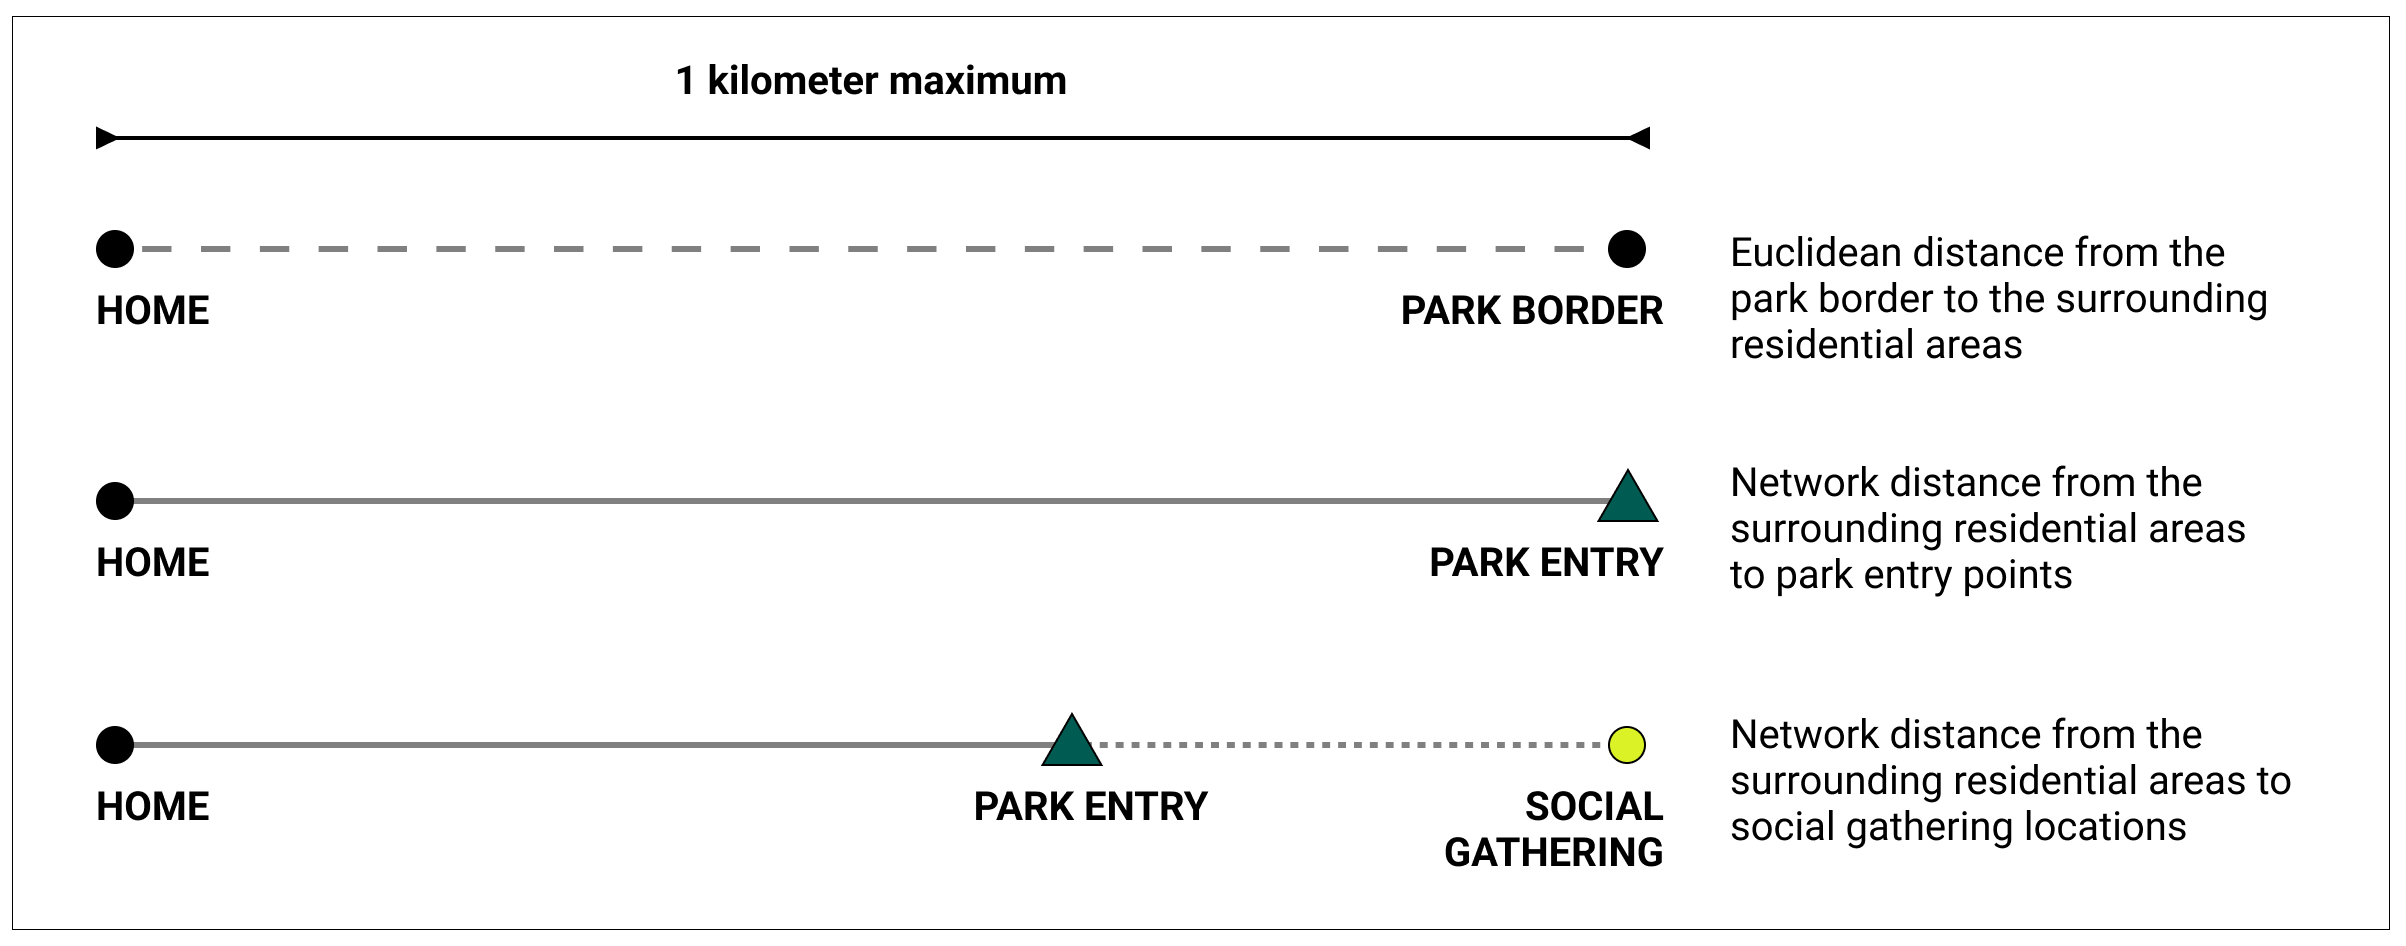
\includegraphics[width=1.0\textwidth]{images/network/network_diagram.png}
  \captionsetup{width=1.0\linewidth}
  \caption[Analysis diagram]{Diagram showing the population studies for three scenarios.}
  \label{fig:concept_diagram}
\end{figure}\par

\begin{multicols}{2}

\section{Population catchment}
\subsection{Measuring access}
To find the number of people with access to the three parks considering the locations of entry points, three calculations are performed: finding the population living within a one-kilometer Euclidean distance of the park border; the population within one-kilometer network distance from park entry points; and finally finding the population of those living within one-kilometer network distance of the social gathering circles (see Figure \ref{fig:concept_diagram}). The population catchment of people living within one-kilometer Euclidean distance of the park border provides a starting point for comparing how the quantity and location of entry points may limit access to the park. Compared to the Euclidean distance population catchment, the population within a one-kilometer network distance of gathering points will be the smallest percentage of the population due to the added distance from entry points to the internal areas of the park where gathering circles are located.

\subsection{Aggregation error}
Governmental census data organized by administrative boundaries is used to approximate the population of residents living near the parks. Ideally, data for the number of residents in individual buildings would be available for a neighborhood-scale analysis; however, this specificity of data is not readily available in all of the cities studied due to privacy protection regulations. Therefore, the population approximation performed below must be qualified by the issue of aggregation error. 

Hewko et al. (2002) describe aggregation error as the inaccuracy of spatial analysis results that occur when areal units are represented by a single point, especially when the specificity of an analysis might necessitate a more accurate distribution of information \cite{hewko_measuring_2002}. When the unweighted centroid of a large municipal boundary such as a zip code in the United States is used to analyze some spatial condition, the single point would not account for a residential zone in one area of the zip code and non-residential zones in another area of the same zip code, giving the false appearance of an evenly distributed population. 

Several measures are taken in this study to avoid inaccuracy of results due to aggregation error. First, the smallest units of governmental census data are used for each city: for Tokyo this is the urban divisions within each ward \begin{CJK}{UTF8}{min}(町丁・字等)\end{CJK}; for New York City the census block is utilized; and the Lower Layer Super Output Area (LSOA) boundaries are used for London. Next, in some of the further analyses completed below, road intersections are combined with divided population data to estimate flow of pedestrians at a more detailed level. 

\end{multicols}

\begin{figure}[ht]
  \centering
  \captionsetup{width=1.0\textwidth}
  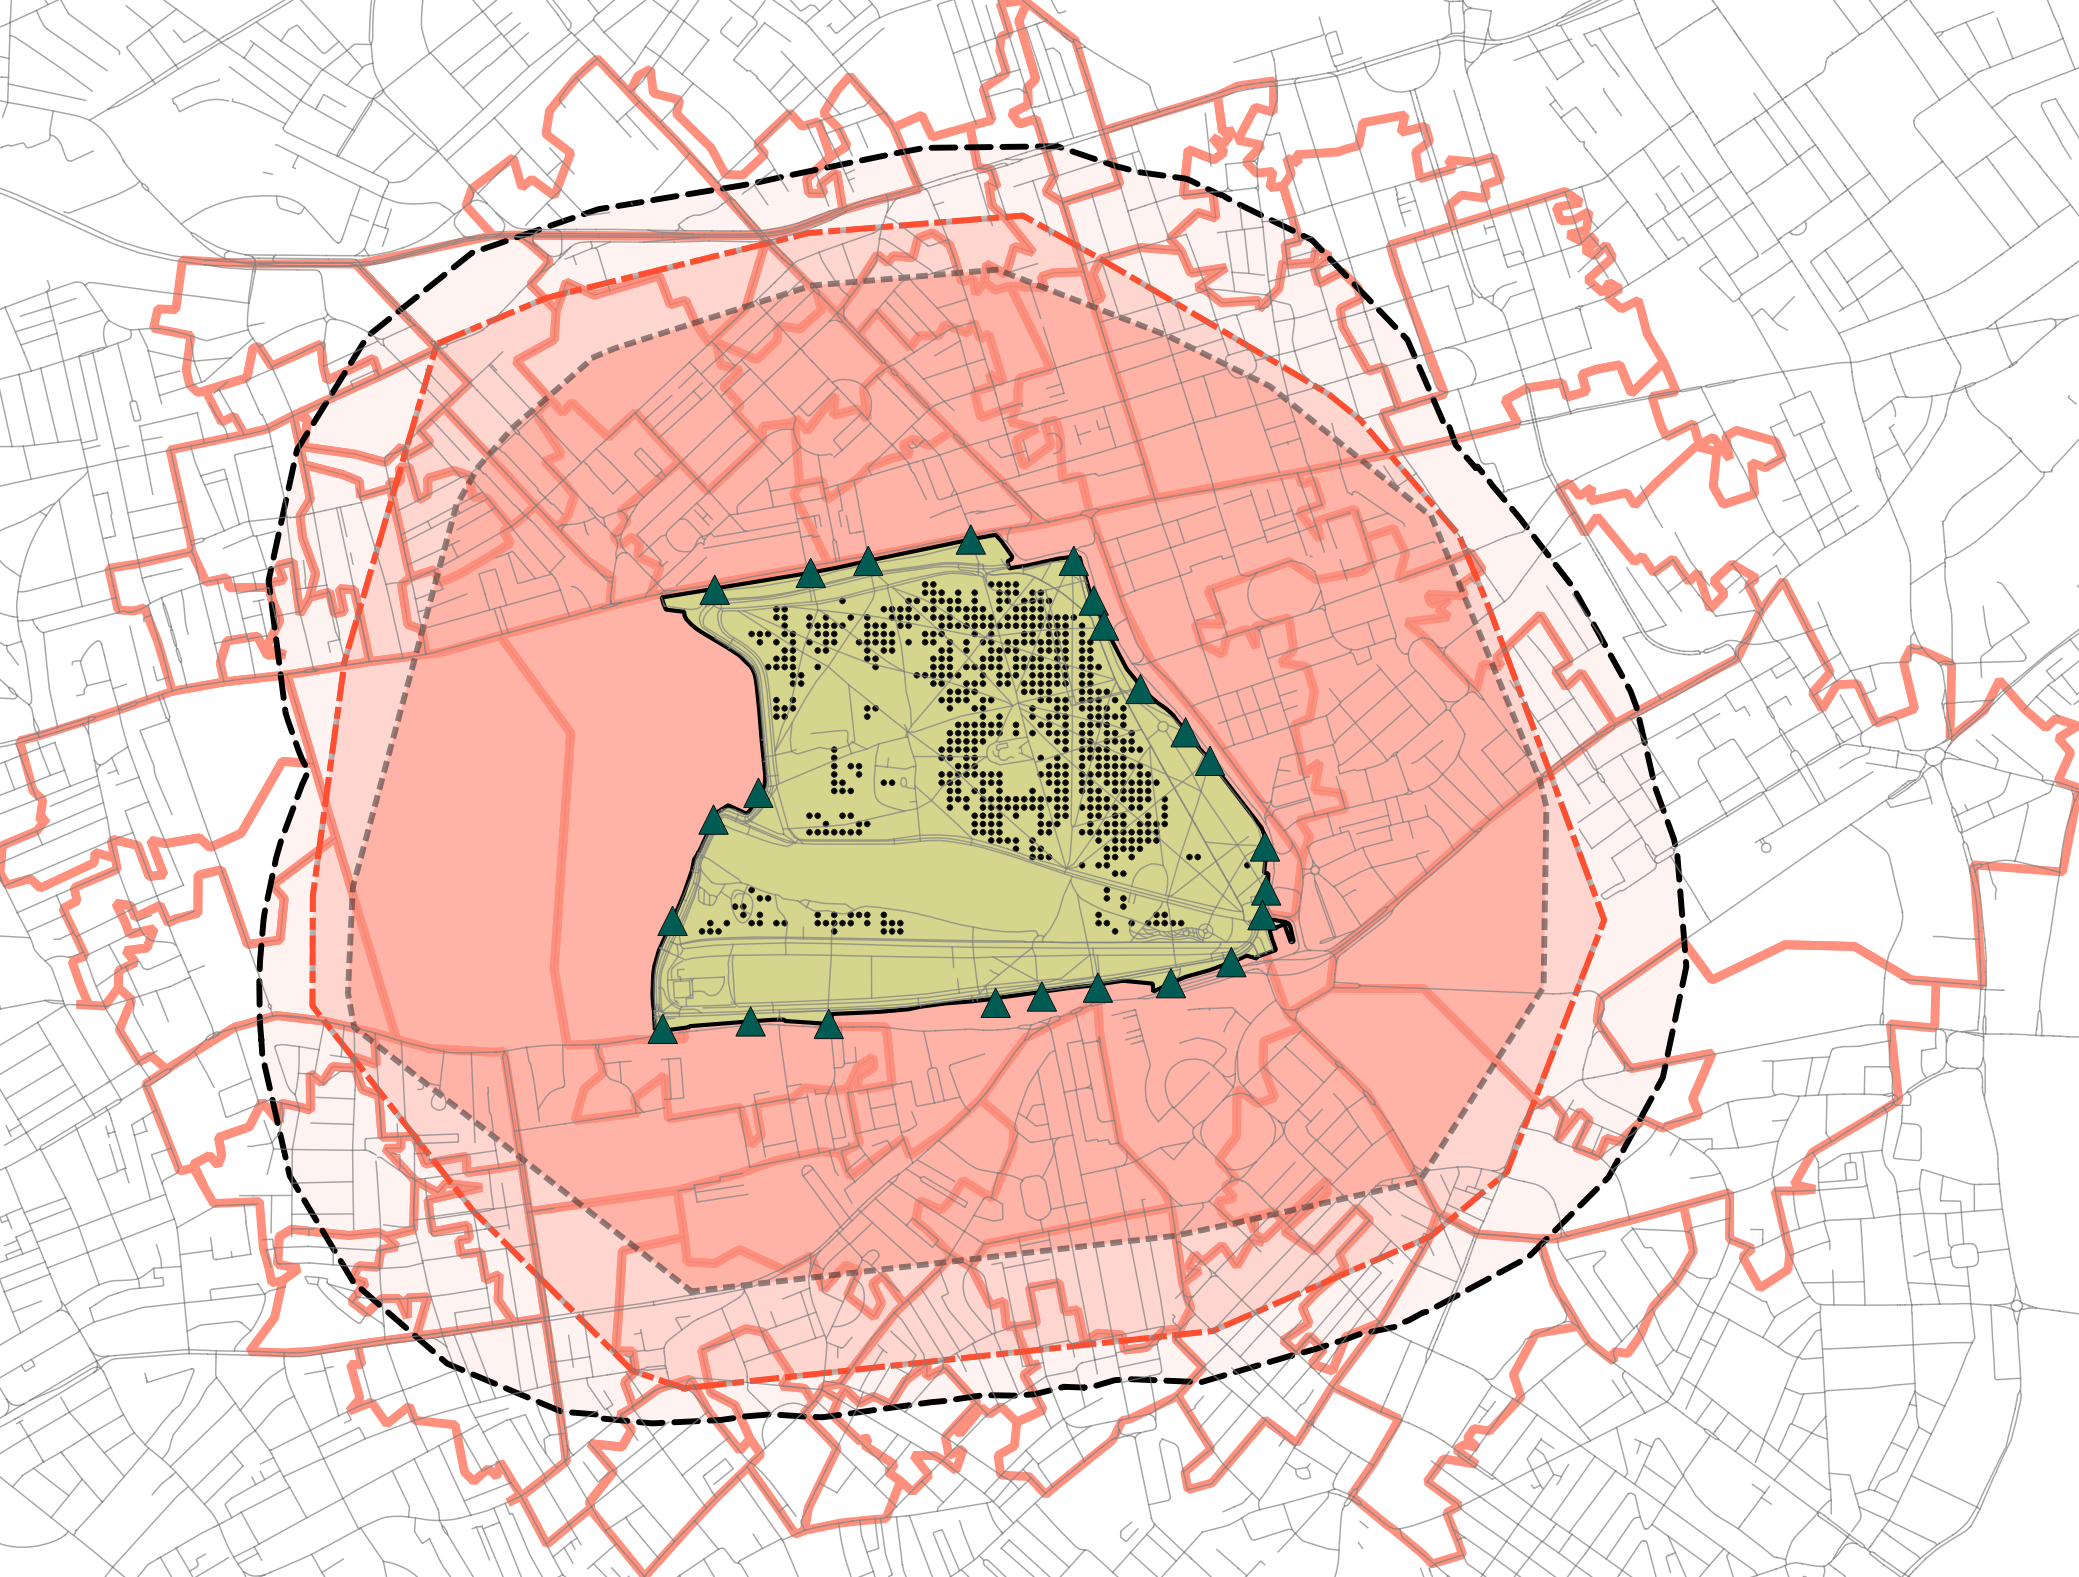
\includegraphics[width=1.0\textwidth]{images/network/hyde_approx_pop.png}\par
  \caption[Hyde Park - population]{Population analysis of Hyde Park.}
  \label{fig:hyde_1km_pop}
\end{figure}

\begin{figure}[ht]
  \centering
  \captionsetup{width=0.8\textwidth}
  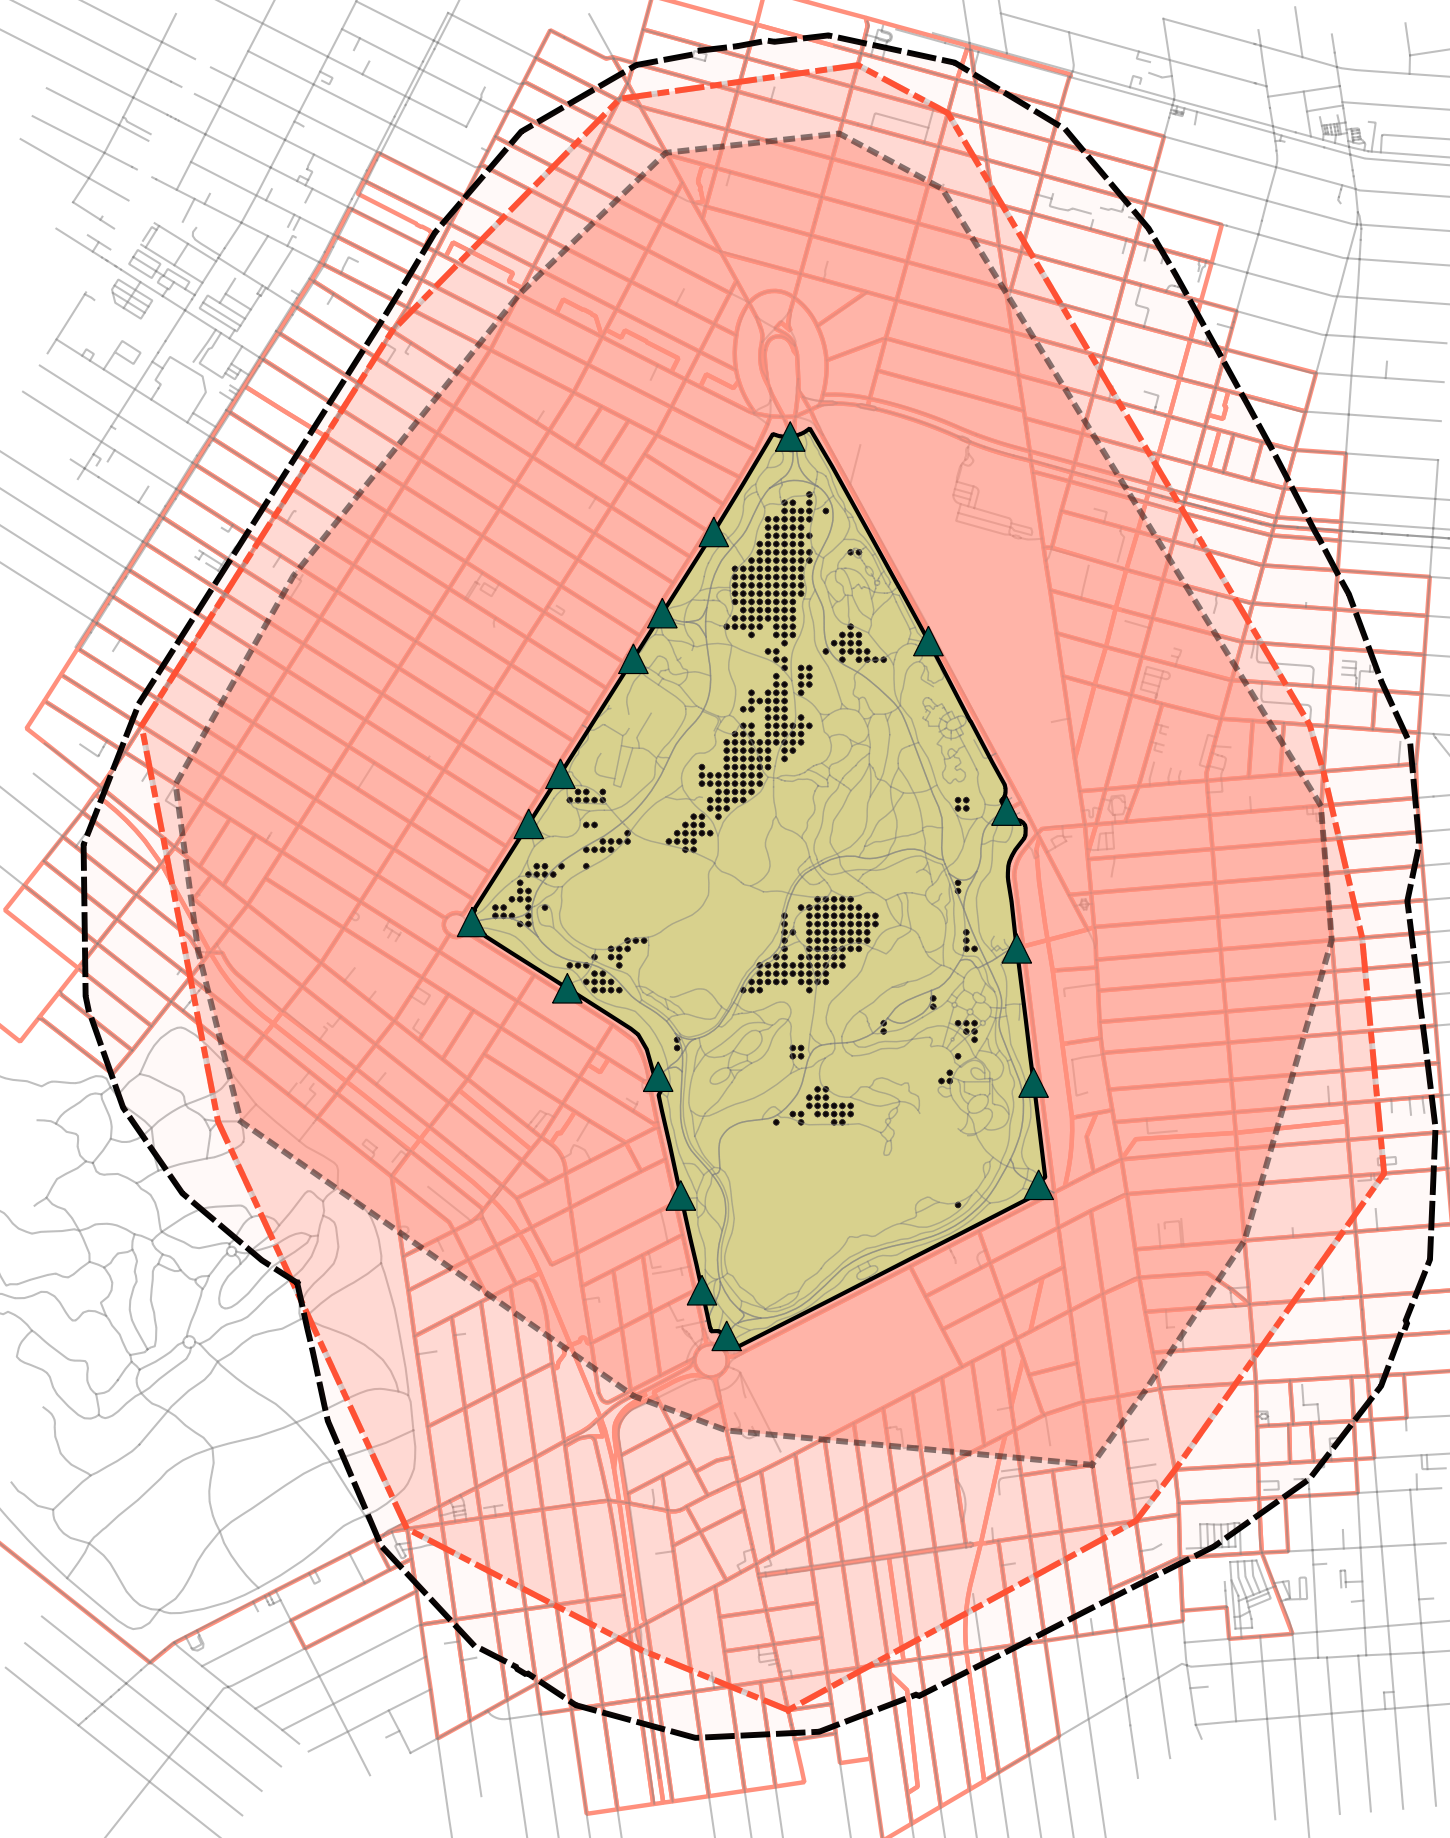
\includegraphics[width=0.8\textwidth]{images/network/prospect_approx_pop.png}\par
  \caption[Prospect Park - population]{Population analysis of Prospect Park.}
  \label{fig:prospect_1km_pop}
\end{figure}

\begin{multicols}{2}

\subsection{Overlap analysis}
A combination of tools is used to approximate the population around Hyde Park, Prospect Park and Yoyogi Park. To begin, government census data is imported into the QGIS software and joined with geographic data for the administrative boundaries. Next, an offset is created from the park border to represent the entire area that is one-kilometer Euclidean distance from the park. The QGIS \textit{Overlap analysis} tool is then utilized to create an approximate population value for each administrative boundary that is within or overlaps the one-kilometer buffer zone around the park based on the percentage of overlap. For example, if a particular administrative boundary falls entirely within the buffer area, the overlap analysis will calculate a value of 100\% and the entire population from that administrative boundary is included. However, if an overlap ratio of 70\% is found, then 70\% of the population for that administrative boundary is included. 

To calculate the number of people living within a one-kilometer network distance of the park entry points, an additional step is required because the centroids of the administrative boundaries could result in aggregation errors as described above. The geographic data is brought into Rhino and the UNA toolbox \textit{Service Area} tool locates the road intersections that are within a one-kilometer network distance of the park entry points. The intersection points are then re-imported into QGIS and the \textit{Minimum bounding geometry} tool creates a convex hull around the points. This convex hull is used in the same way that the one-kilometer Euclidean buffer polygon was used above to approximate the population based on the overlapping administrative boundaries and associated population.

\begin{figure}[H]
  \centering
  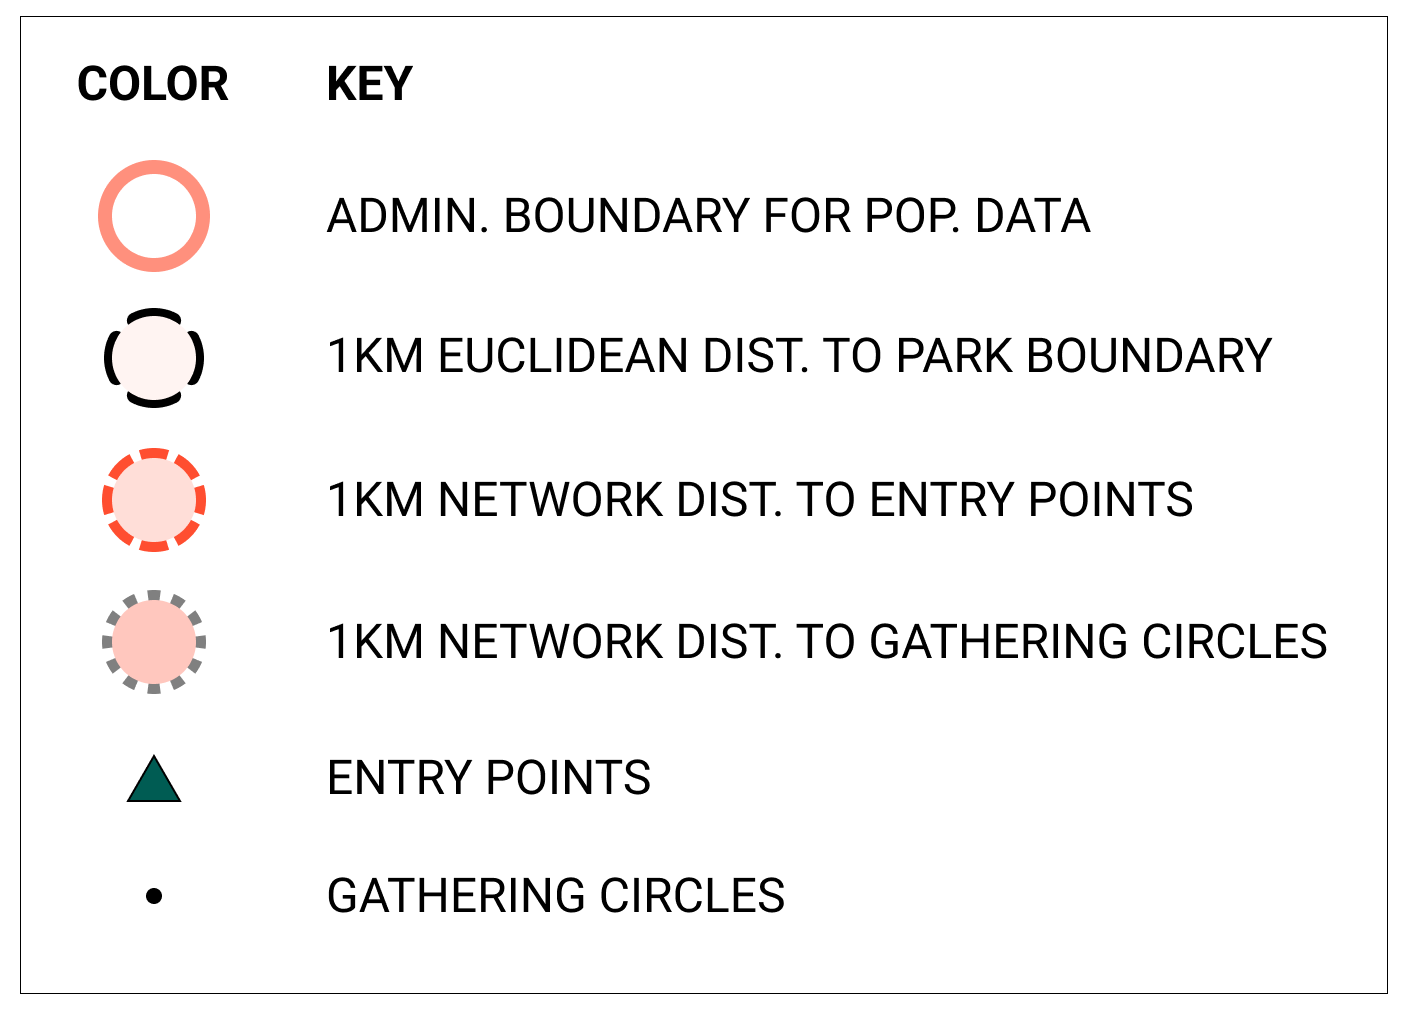
\includegraphics[width=0.45\textwidth]{images/network/approx_pop_legend.png}\par\captionof{figure}[Population legend]{Analysis of population.}
  \label{fig:approx_pop_legend}
\end{figure} 

\end{multicols}

\begin{figure}[ht]
  \centering
  \captionsetup{width=0.8\textwidth}
  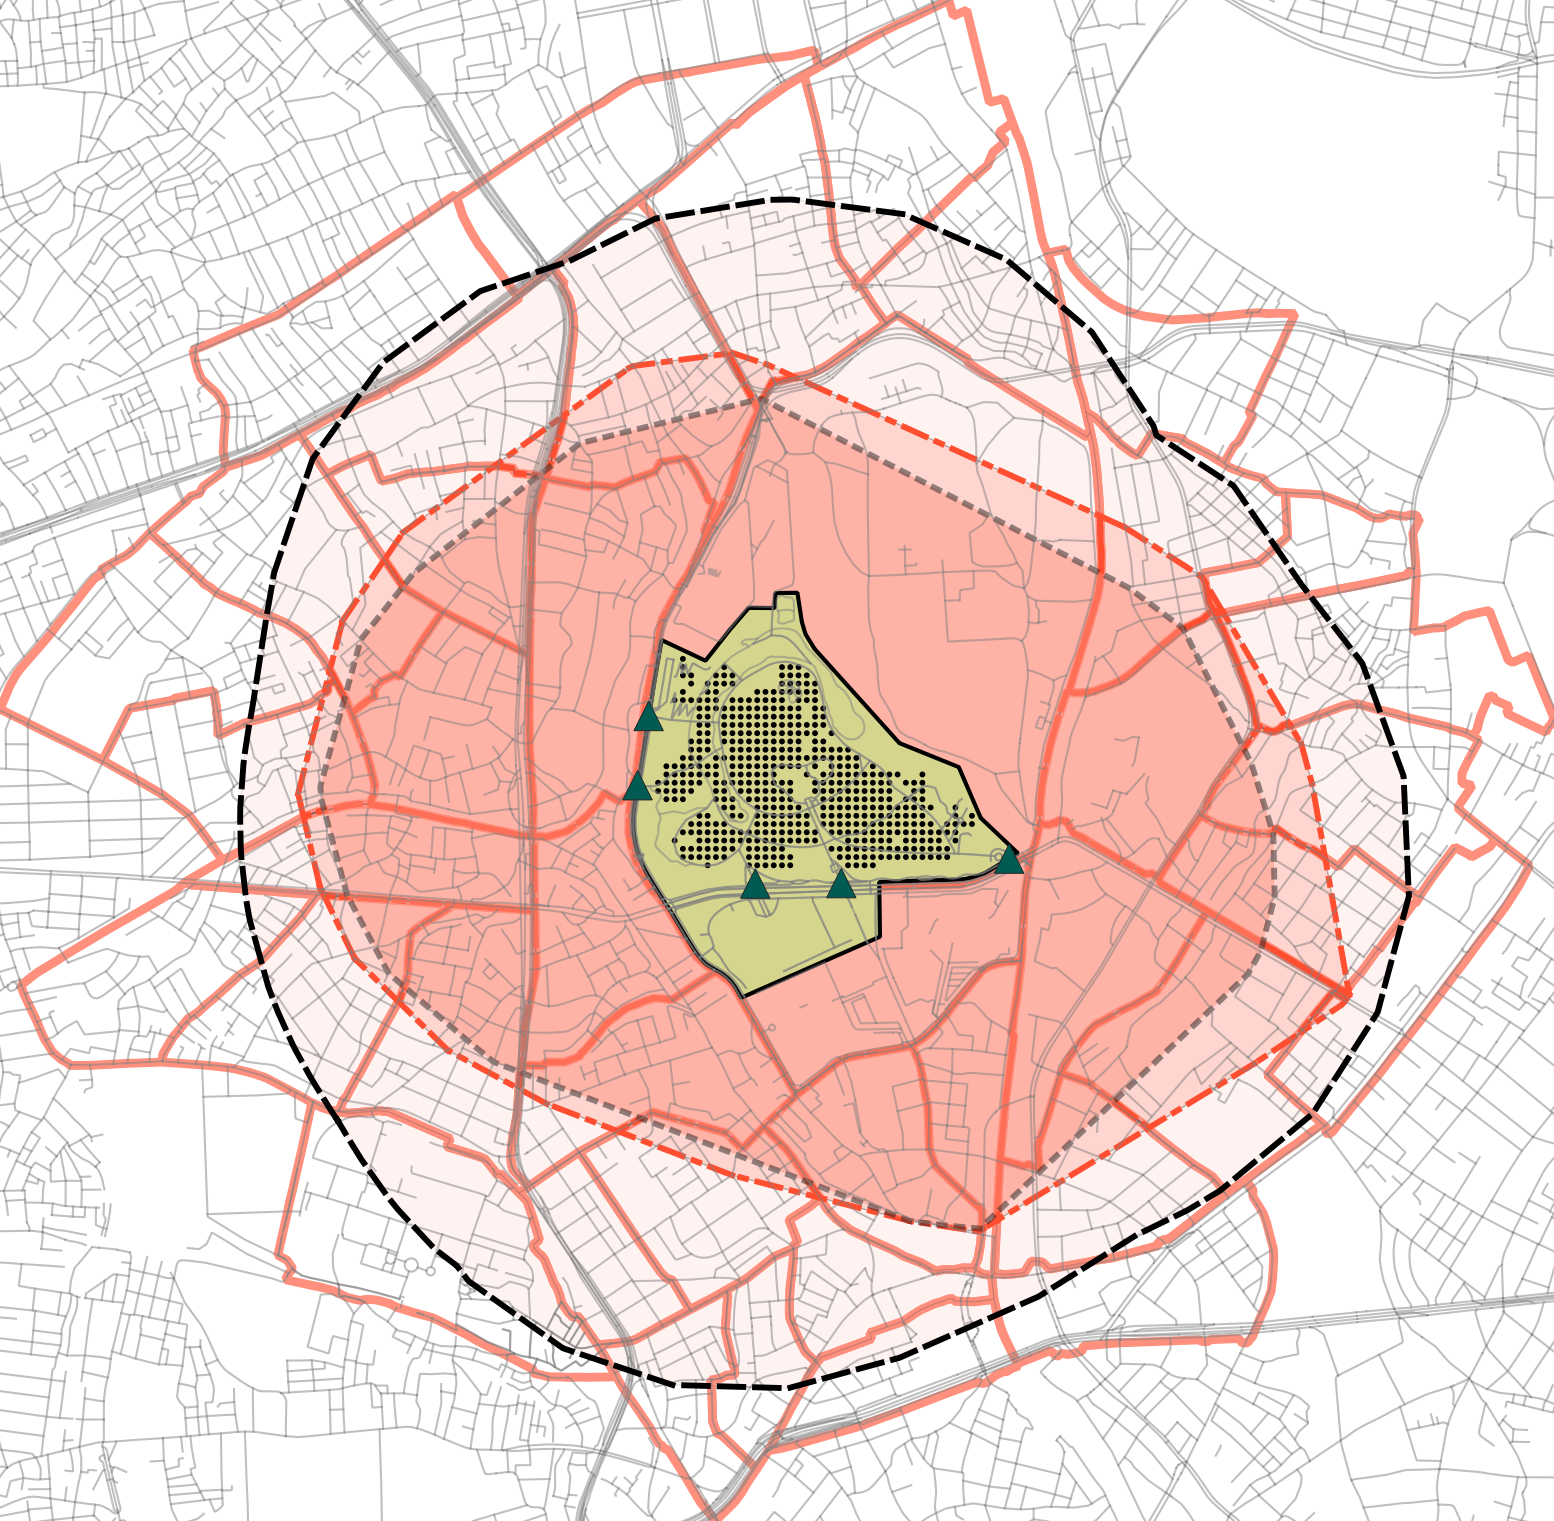
\includegraphics[width=0.8\textwidth]{images/network/yoyogi_approx_pop.png} \\
  \vspace{10pt}
  \caption[Yoyogi Park - population]{Population analysis of Yoyogi Park.}
  \label{fig:yoyogi_1km_pop}
\end{figure}

\begin{table}[h]
\centering
\small
\begin{tabular}{lcccccr}
\toprule
{} &  1km to border &    {} &  1km to entries &   {} &  1km to gatherings &   {} \\
Park name &  (Euclid.) &    Pct. &  (network) &   Pct. &  (network) &   Pct. \\
\midrule
Hyde Park &         58414 &  100.0\% &                39075 &  67.0\% &                  26925 &  46.0\% \\
Prospect Park &        194962 &  100.0\% &               156423 &  80.0\% &                 111315 &  57.0\% \\
Yoyogi Park &         81488 &  100.0\% &                43312 &  53.0\% &                  34786 &  43.0\% \\
\bottomrule
\end{tabular}
\caption[Approximate population]{Approximate population.}
\label{table:approx_pop}
\end{table}

\begin{multicols}{2}

\begin{minipage}{0.45\textwidth}
    \centering
    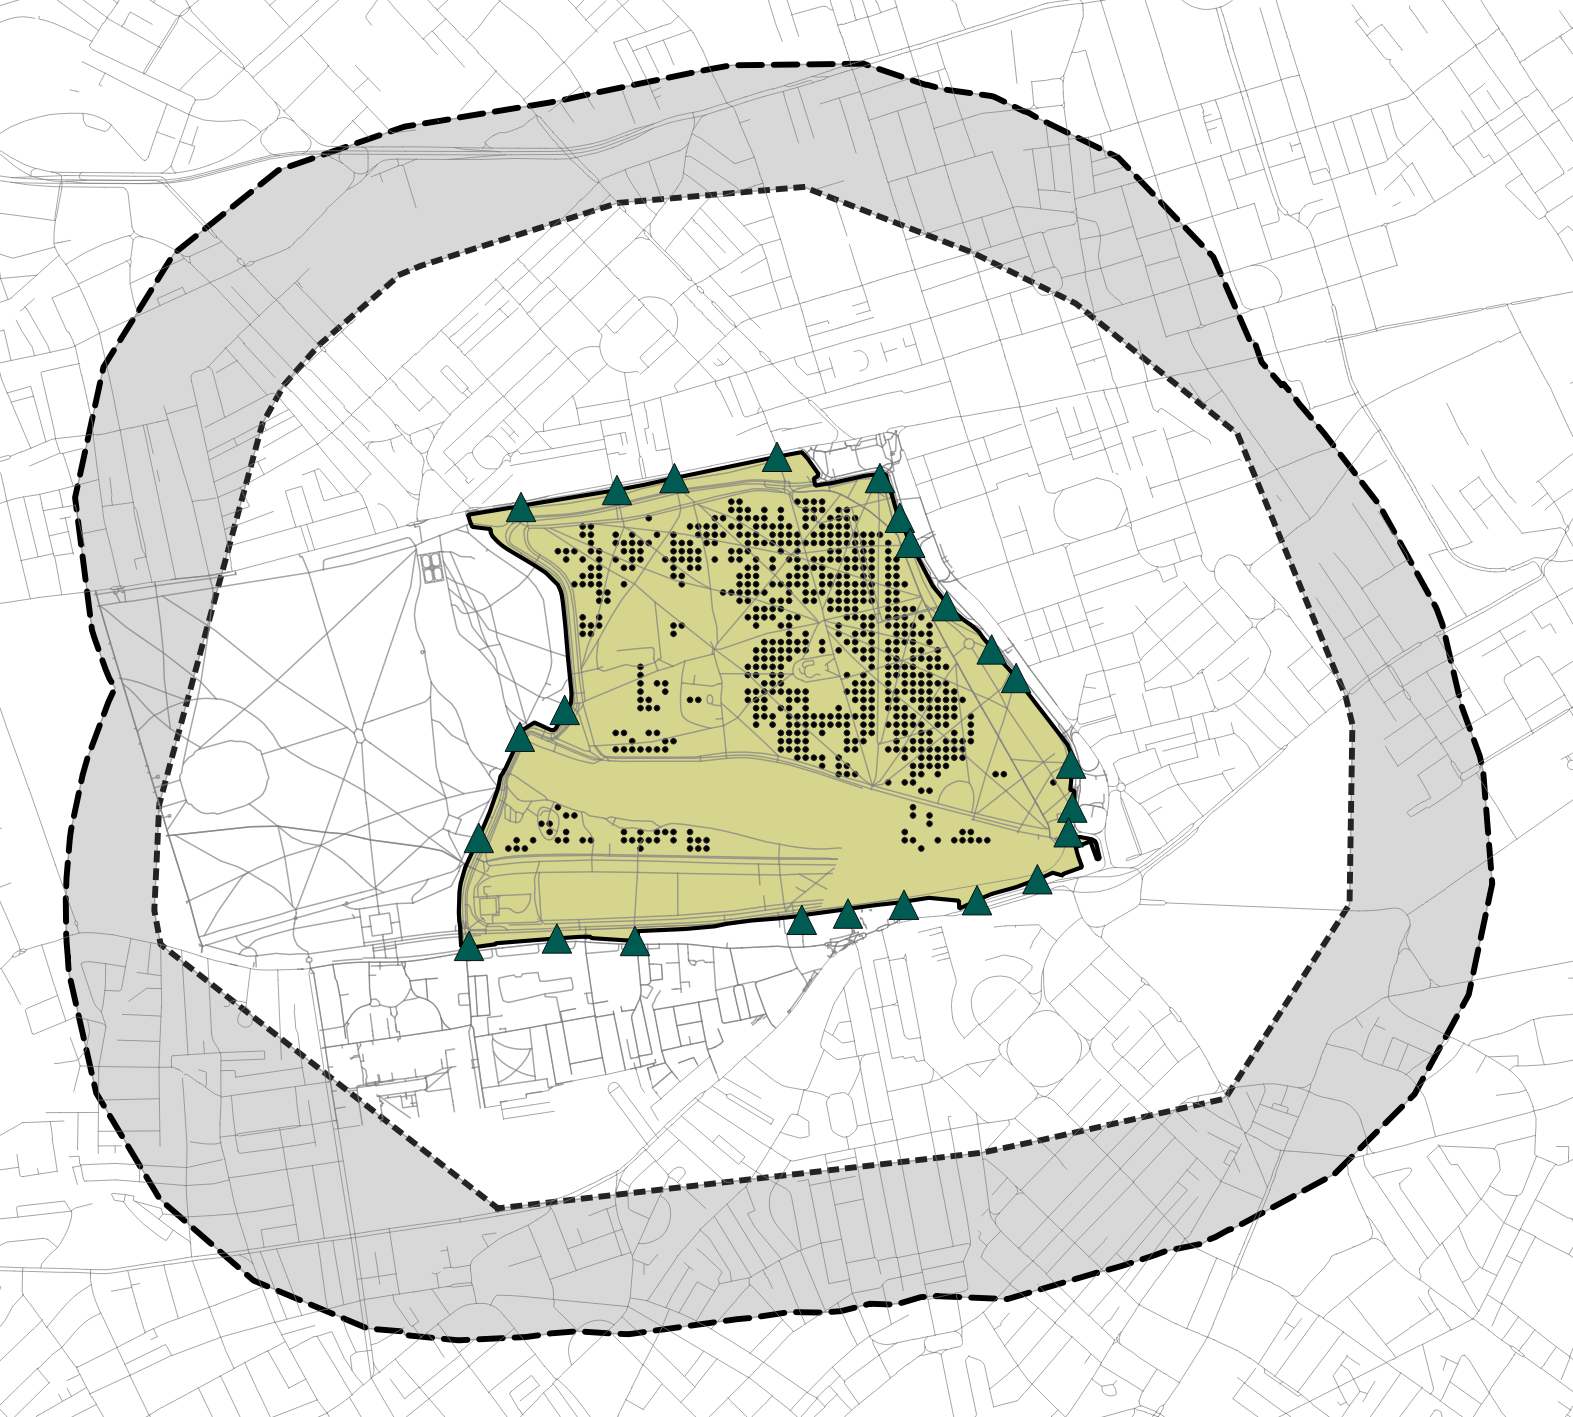
\includegraphics[width=\linewidth]{images/network/hyde_difference.png}\par\hspace{5pt} % add a small amount of horizontal space between images%
    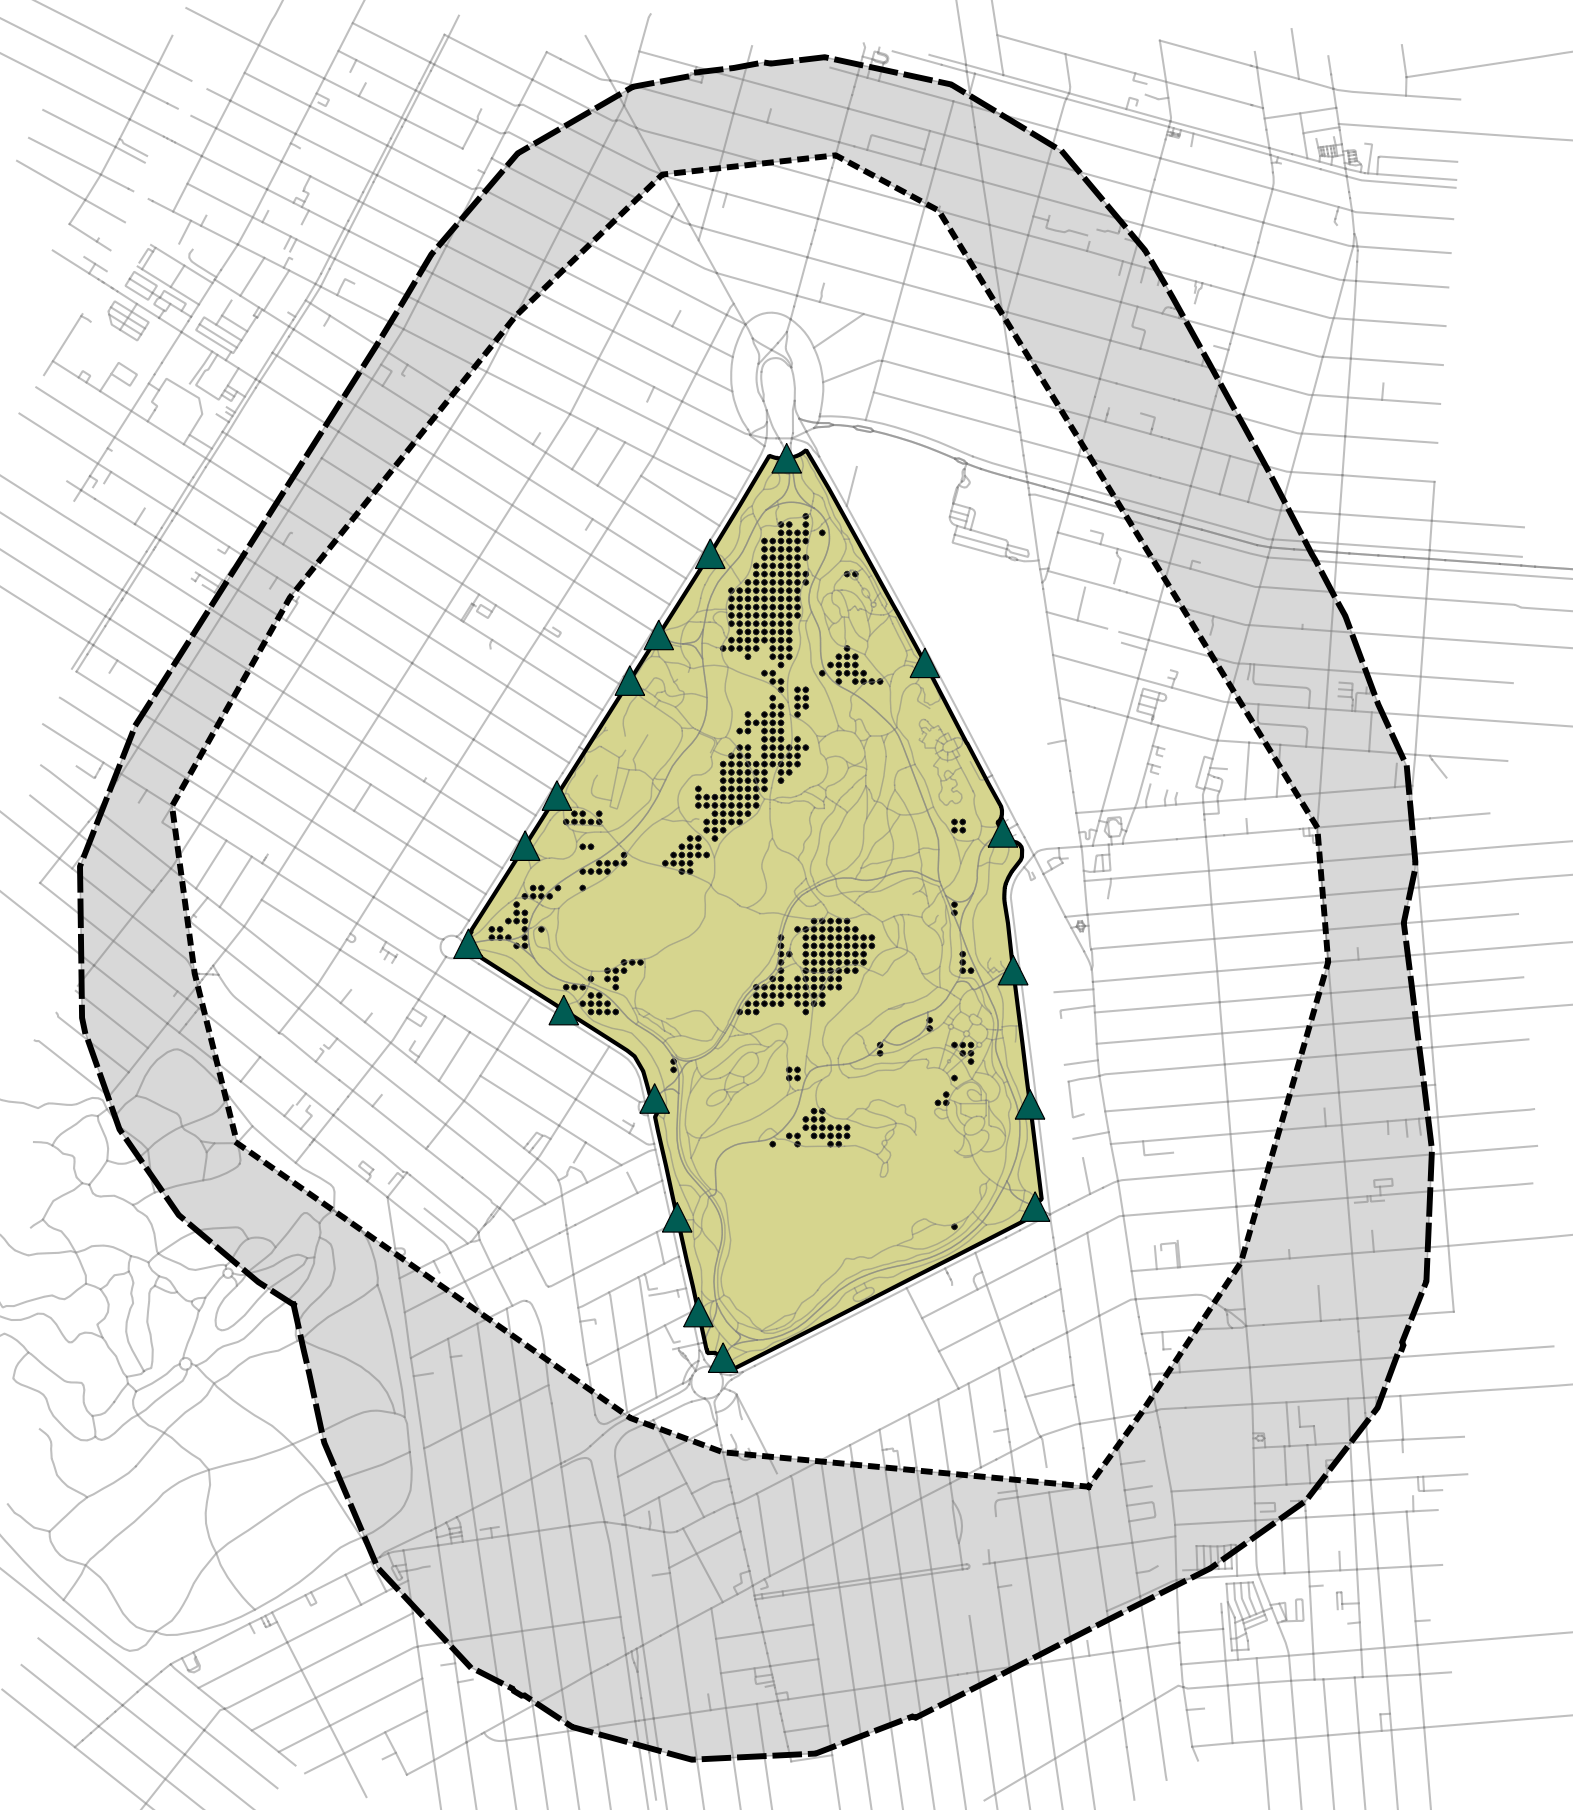
\includegraphics[width=\linewidth]{images/network/prospect_difference.png}\par\hspace{5pt} % add a small amount of horizontal space between images
    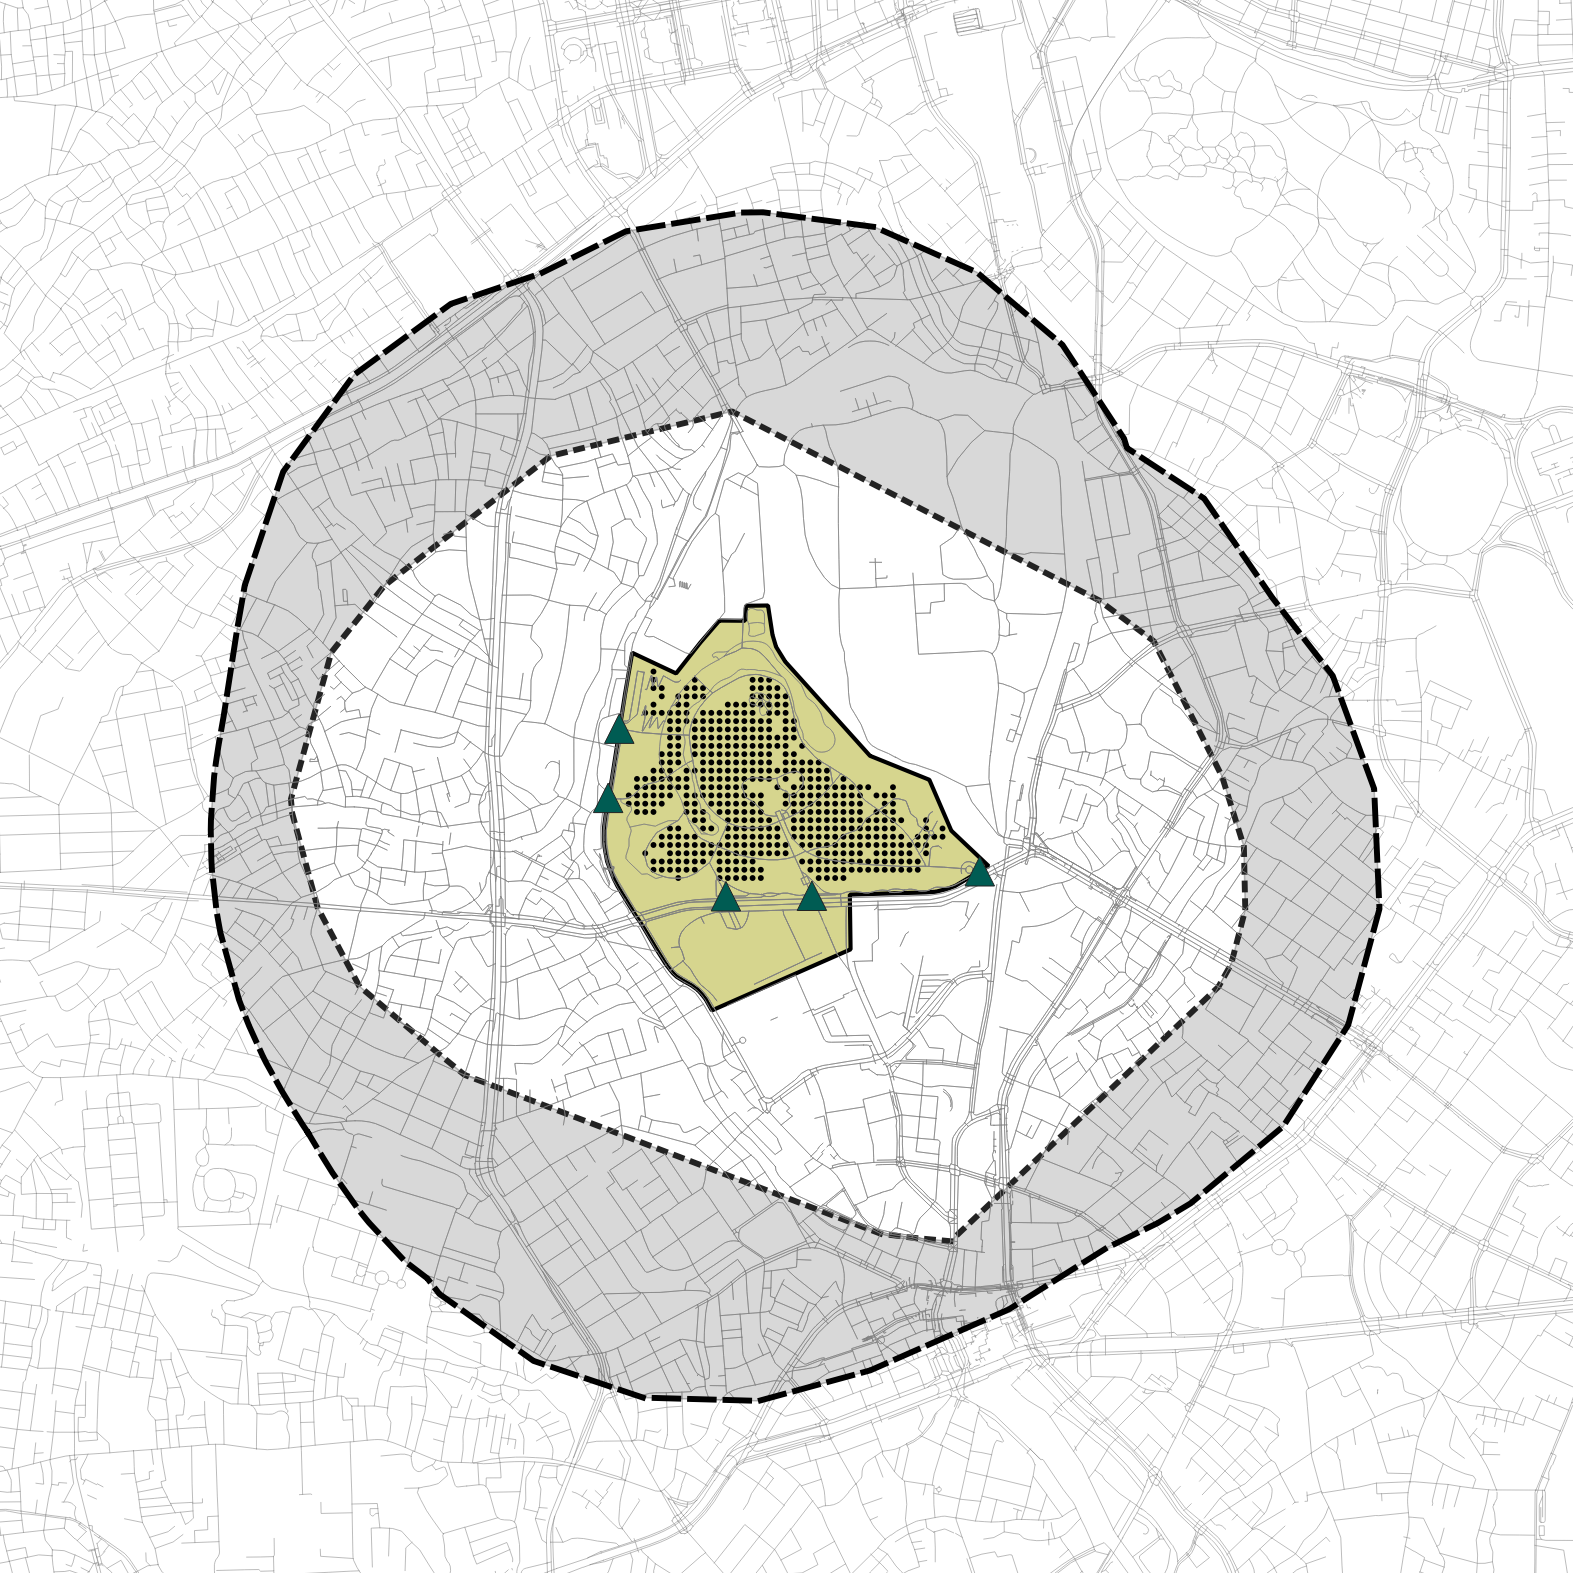
\includegraphics[width=\linewidth]{images/network/yoyogi_difference.png}\par\hspace{5pt} % add a small amount of horizontal space between images
    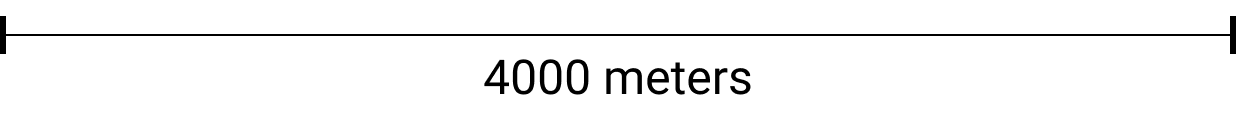
\includegraphics[width=\linewidth]{images/network/scale_legend_5.png}\par\captionof{figure}[Difference]{Top to bottom: Hyde Park, Prospect Park, and Yoyogi Park. Difference in area between Euclidean distance and network distance.}
    \label{fig:network_diff}
\end{minipage}

\subsection{Approximate populations}\label{approx_pop}
The results of the population analysis can be seen in Table \ref{table:approx_pop} and in Figures \ref{fig:hyde_1km_pop}-\ref{fig:yoyogi_1km_pop}. When a one-kilometer straight-line (Euclidean) distance is considered to be 100\% of the population living around the park, then the percentage calculated for one-kilometer network distance to the entry points and gathering circles can be analyzed for how accessibility decreases when considering the road network. 

For example, the population of people living around Hyde Park decreases by 33\% when considering the difference between those who live one-kilometer straight-line distance to the park border compared to those who live a network distance of one-kilometer to a park entry point. Then, when looking at those who live within one-kilometer network distance to the closest social gathering circle, the percentage of the original population decreases to 46\%. For Hyde Park, one of the main reasons for this decrease in the accessible population is the geographic positioning next to Kensington Gardens, which is another large green space. This means that no one lives directly west of the park, limiting access to those who live north, east, and south of the park (see Figure \ref{fig:hyde_1km_pop}). 

Prospect Park, on the other hand, sees the smallest decrease in population when comparing straight line distance to network distance. The population living within one-kilometer network distance of entry points is only 20\% less than the straight-line distance population; and those living within one-kilometer of social gathering areas consist of 57\% of the originally calculated population. While Prospect Park is adjacent to the Brooklyn Botanic Garden and Parade Ground, neither of those zones interfere with the population catchment in the same way as the adjacent green spaces to Hyde Park and Yoyogi Park. One interesting observation is that the southern area of Prospect Park is lacking in social gathering spots compared to the northern area. Therefore, in Figure \ref{fig:prospect_1km_pop} there is a large difference in the polygon that represents the network distance to park entry points and the polygon representing the network distance to social gathering circles. 

The findings for Yoyogi Park show the largest discrepancy between straight-line distance and network distances. The population within one-kilometer network distance to entry points decreases by almost fifty percent (47\%). Moreover, from the surrounding areas to the gathering areas, only 43\% of the original population in the straight-line buffer have access to social gathering circles within a one-kilometer walk. Due to both the green space to the north of the park dedicated to Meiji-Jingu Shrine and the limited number of entry points, the areas to the north and south of Yoyogi Park show the greatest loss of access to entry points and gathering circles compared to the straight line distance from the park borders (see Figure \ref{fig:yoyogi_1km_pop}).

Figure \ref{fig:network_diff} shows the difference in geographical areas between the Euclidean one-kilometer buffer around the park borders, and the area within which the residents can get from home to a social gathering circle in less than a one-kilometer. In other words, the gray filled regions represents the zone where residents live within a one-kilometer straight line distance from a park entry, but they are not within one-kilometer network distance of social gathering circles. Despite having the largest percentage of gathering circles to the total park area as found in Chapter \ref{chapter_04}, Yoyogi Park has the greatest reduction in population when comparing straight line distance and network distance. Prospect Park has the least significant reduction in population, but it does have one area that is particularly of concern to the south of the park as seen in the middle image of Figure \ref{fig:network_diff}. This expansion of the gray area is due not to lack of entry points, but to the lack of social gathering circles identified in the southern region of the park.

\section{Reach analysis}
\subsection{Closest facility}
The distribution of population and social gatherings to the respective nearest entry points is compared in order to understand how the quantities of social gatherings relate to the population of people living nearby. The \textit{Closest Facility} tool in the UNA toolbox locates the destination point that is closest to each origin point along the network, and calculates the \textit{Reach} value at the destinations \cite{sevtsuk_urban_2012}. The UNA toolbox was created with pedestrian and cyclist traffic in mind, yet the reach analysis formula is the same for both vehicular and foot-traffic according to Sevtsuk (2012). 

The \textit{Reach} formula used in the UNA toolbox is defined as:\\

\begin{equation}
        \textit{Reach}[\textit{i}]^{\textit{r}} = \sum_{\textit{j}\in\textit{G}-\{\textit{i}\},\textit{d}[\textit{i},\textit{j}]\le\textit{r}} \textit{W}[\textit{j}]
        \label{eqn:simple_eqn}
\end{equation} \\

Where \textit{d}[\textit{i},\textit{j}] is the shortest path distance between the Origin points \textit{i} and the Destination points \textit{j} along the network \textit{G}. \textit{W}[\textit{j}] is the weight of Destination points \textit{j}. In this study the destination weight is the approximated population from Section \ref{approx_pop}, as well as a count of gathering circles and food amenities in the reach studies that follow \cite{sevtsuk_urban_2012}. 

\subsection{Reach of population and gatherings}\label{reach}
The \textit{Reach} value for the approximate population is calculated using the \textit{Closest Facility} tool as described above. The centroids of the administrative boundaries for the census data are the origin points and the park entries are the destination points where the reach value is summed. The output is a line connecting the centroid to the closest entry, and the approximate population value from that administrative boundary is added to the entry point as an attribute. The same sequence of analysis is completed for the social gatherings circles within the parks to the entry points. 

A maximum network distance of one-kilometer is input into the tool parameters, but the points used in this calculation are only those representing the population the living within one-kilometer network distance to social gathering circles. The sum of the population closest to each entry points can be seen in Figure \ref{fig:nearest_entries}. Figure \ref{fig:nearest_gatherings} shows the distribution of gathering spaces to their respective closest entry points. The summed reach values at each entry point show the total number of gathering circles calculated in Chapter \ref{chapter_04} distributed to the closest entry points along the network. The gathering circles were simplified for the analysis, where one point is equal to roughly twenty-five social gathering circles, but the labels in Figure \ref{fig:nearest_gatherings} show the total number of gathering circles.

\begin{minipage}{0.45\textwidth}
    \centering
    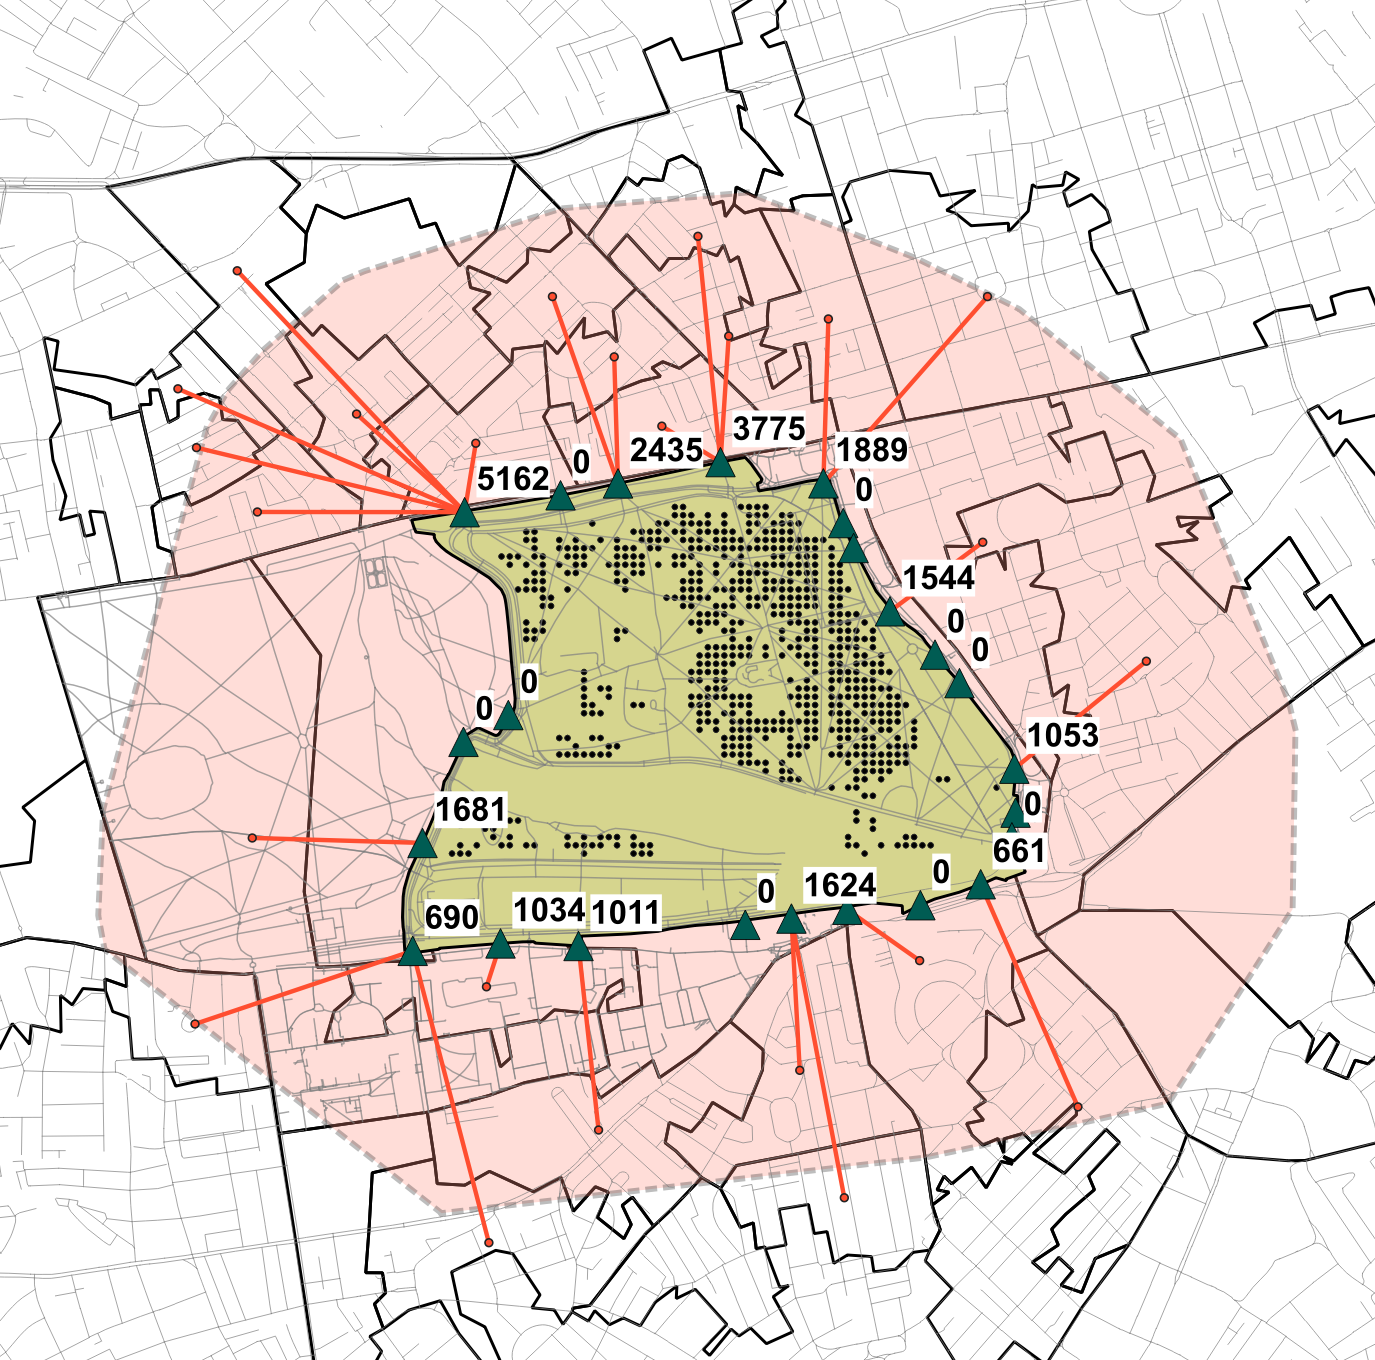
\includegraphics[width=\linewidth]{images/network/hyde_census_nearest.png}\par\hspace{3pt} 
    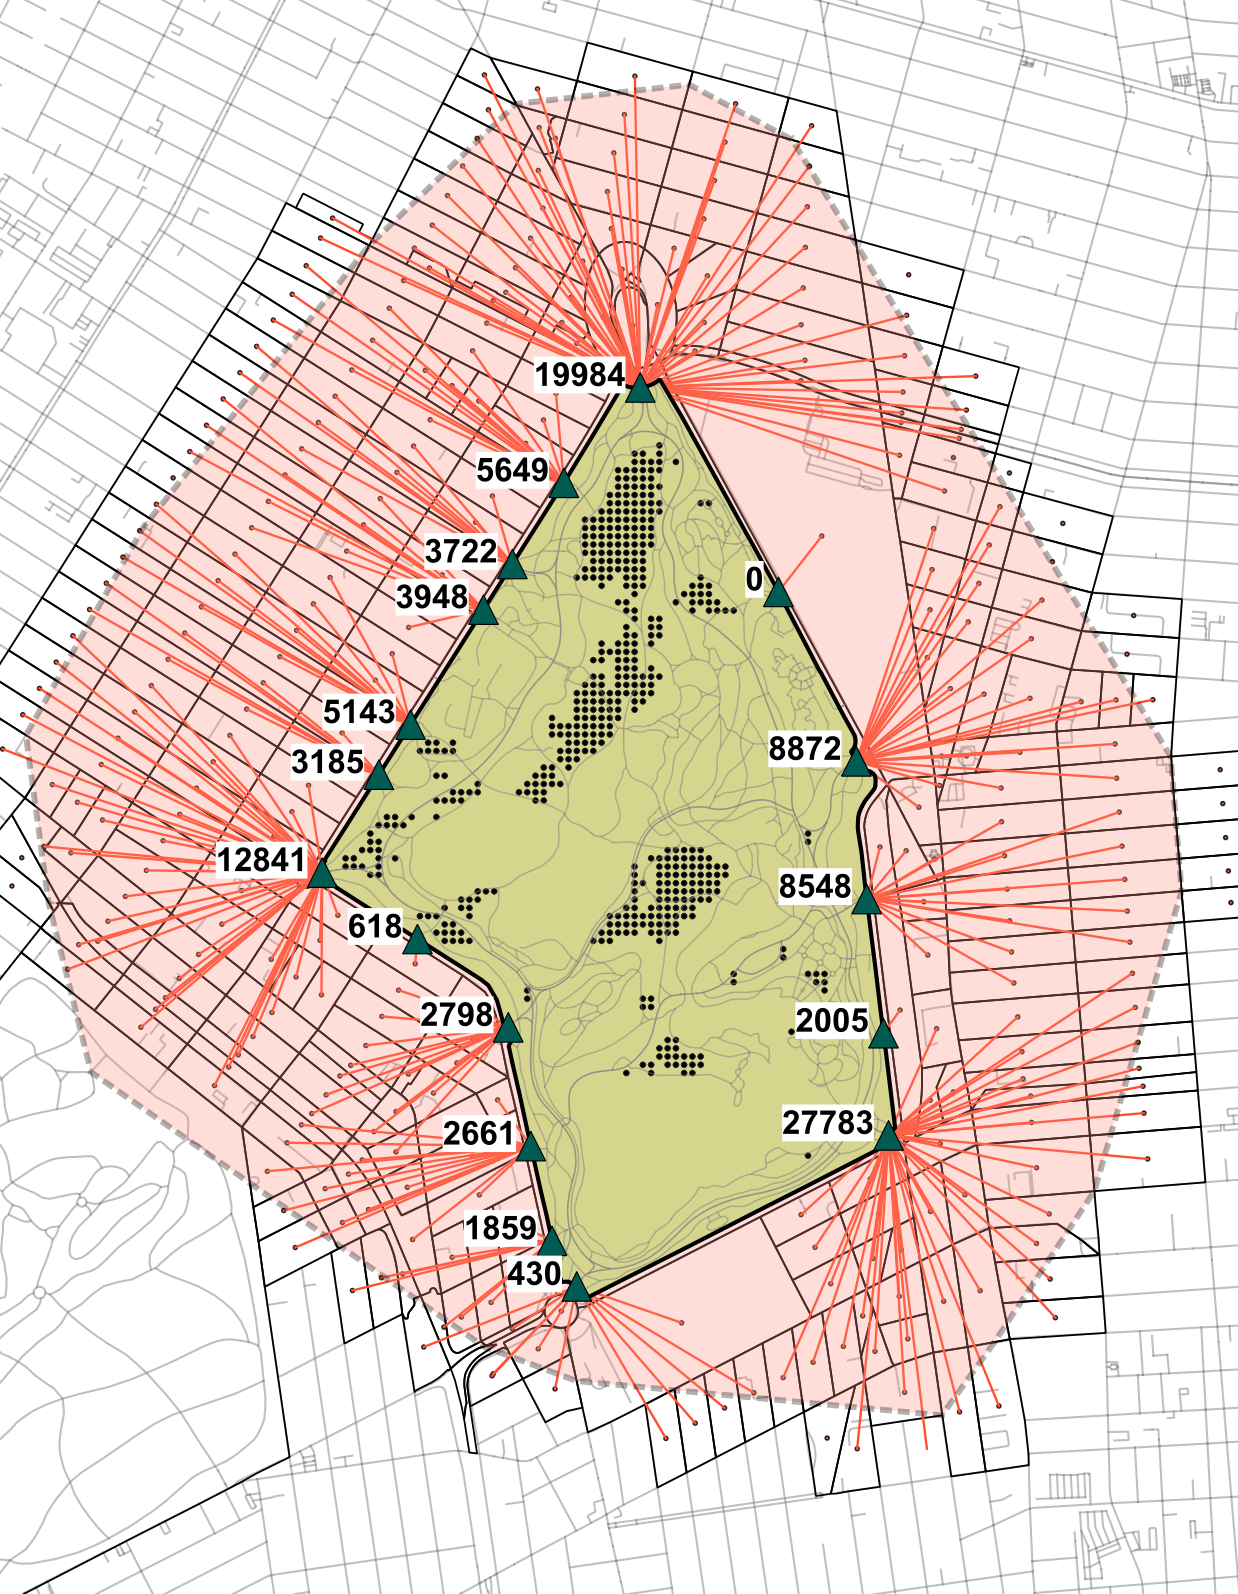
\includegraphics[width=\linewidth]{images/network/prospect_census_nearest.png}\par\hspace{3pt}
    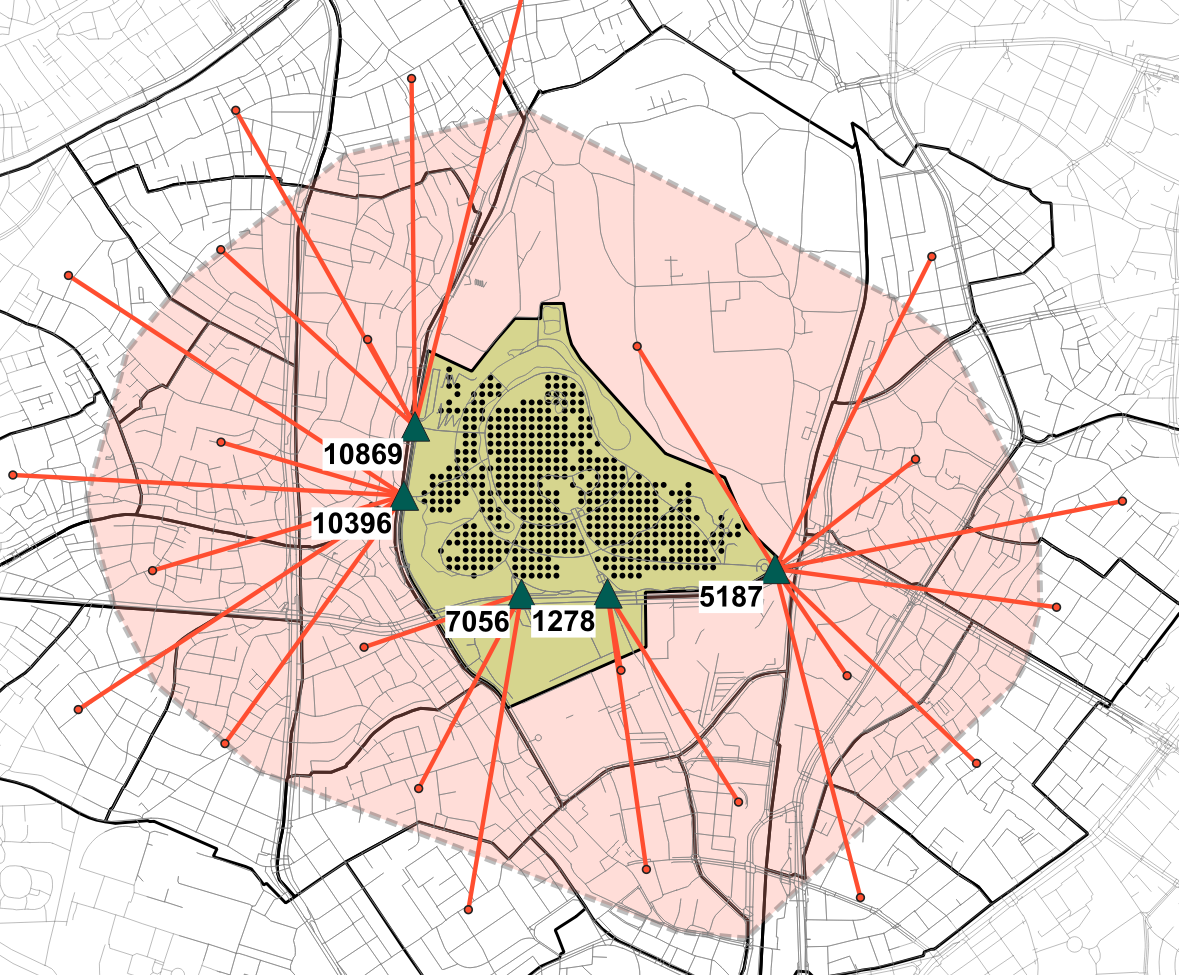
\includegraphics[width=\linewidth]{images/network/yoyogi_chome_nearest.png}\par\hspace{3pt}
    \par\captionof{figure}[Census blocks to closest entries]{Top to bottom: Hyde Park, Prospect Park, and Yoyogi Park. Approximate population based on the closest entry point to the center point of each census block.}
    \label{fig:nearest_entries}
\end{minipage}

\begin{minipage}{0.45\textwidth}
    \centering
    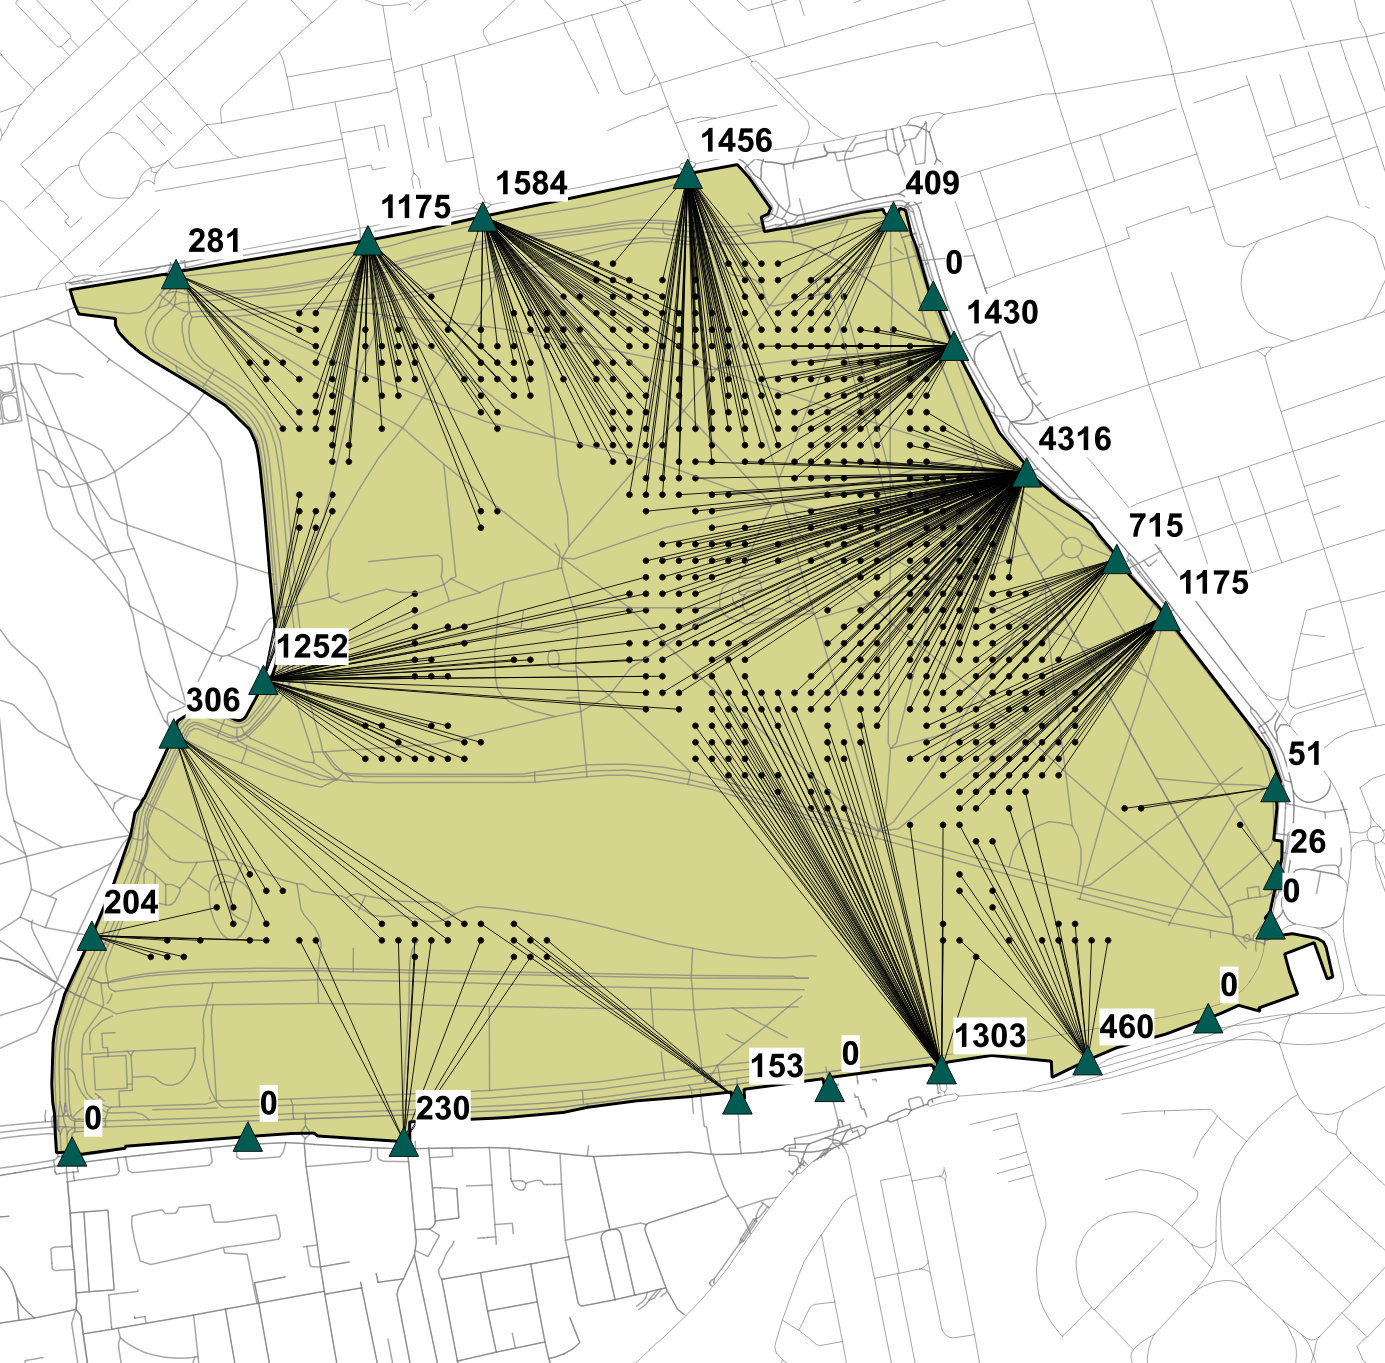
\includegraphics[width=\linewidth]{images/network/hyde_gatherings_nearest.png}\par\hspace{3pt} 
    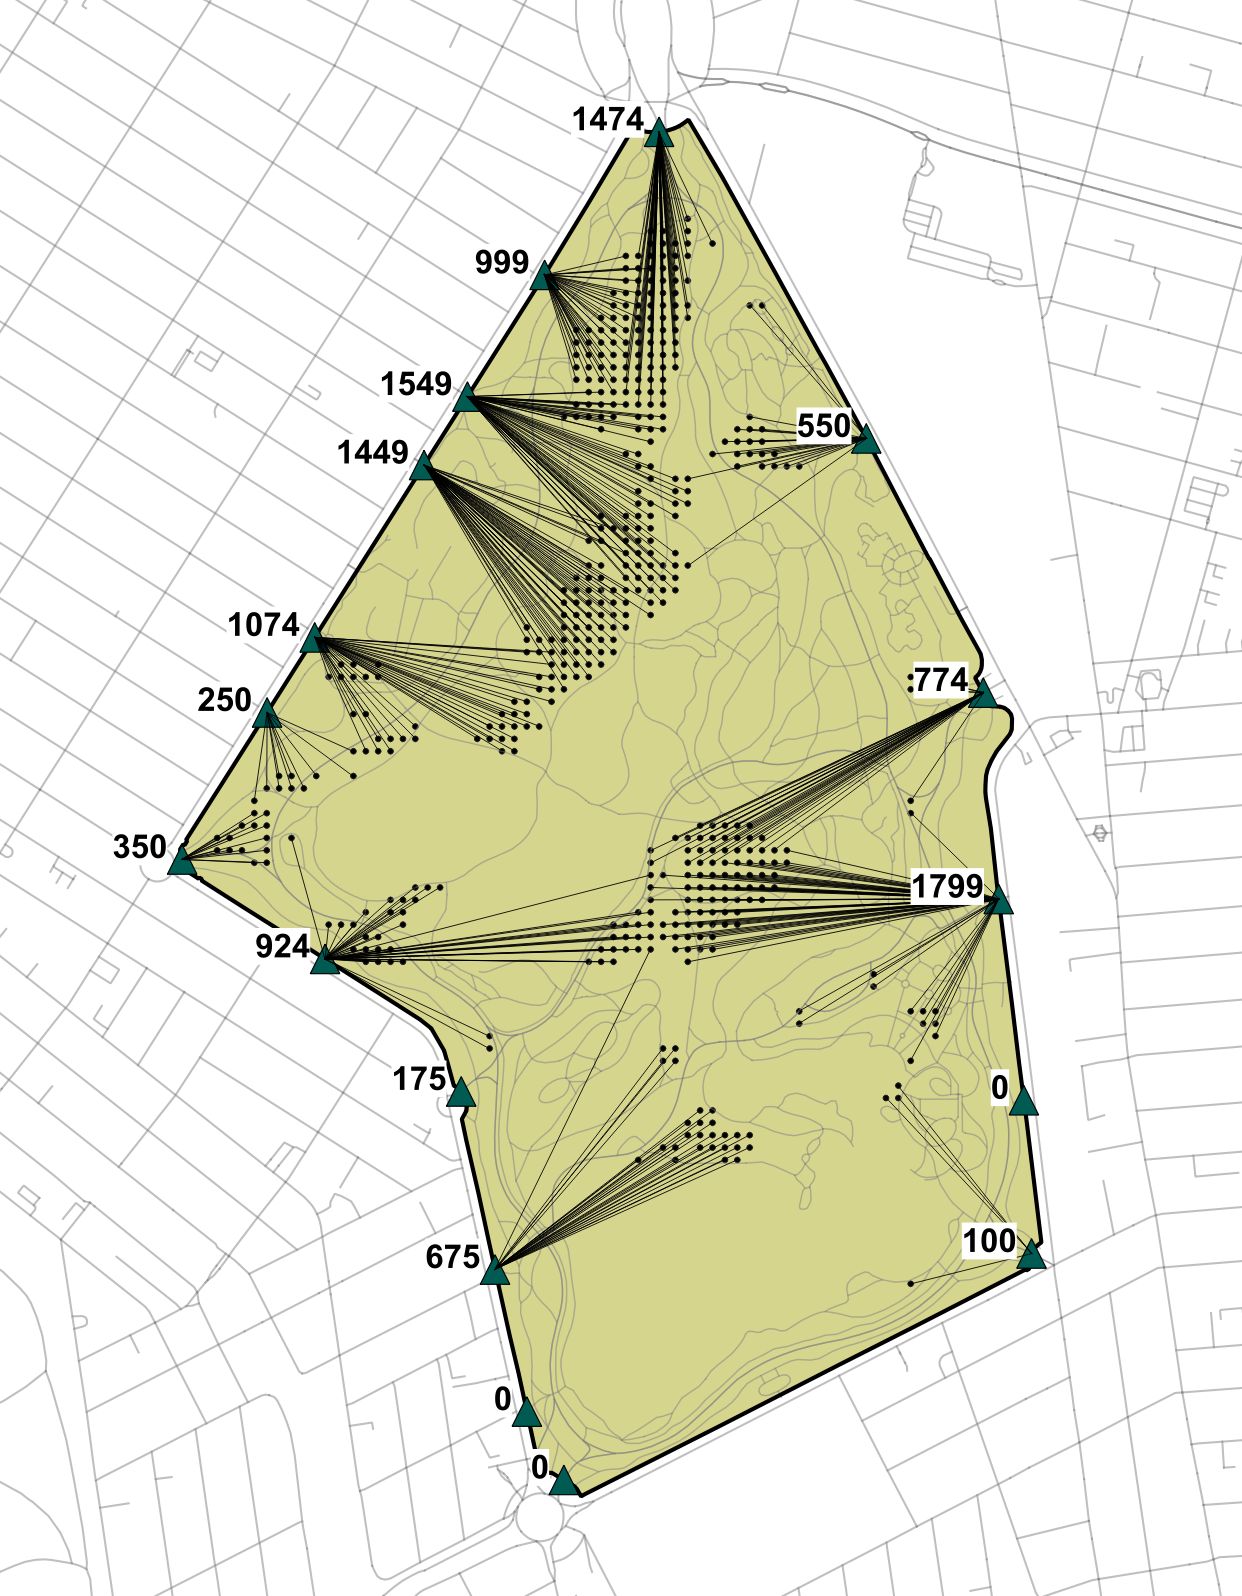
\includegraphics[width=\linewidth]{images/network/prospect_gatherings_nearest.png}\par\hspace{3pt}
    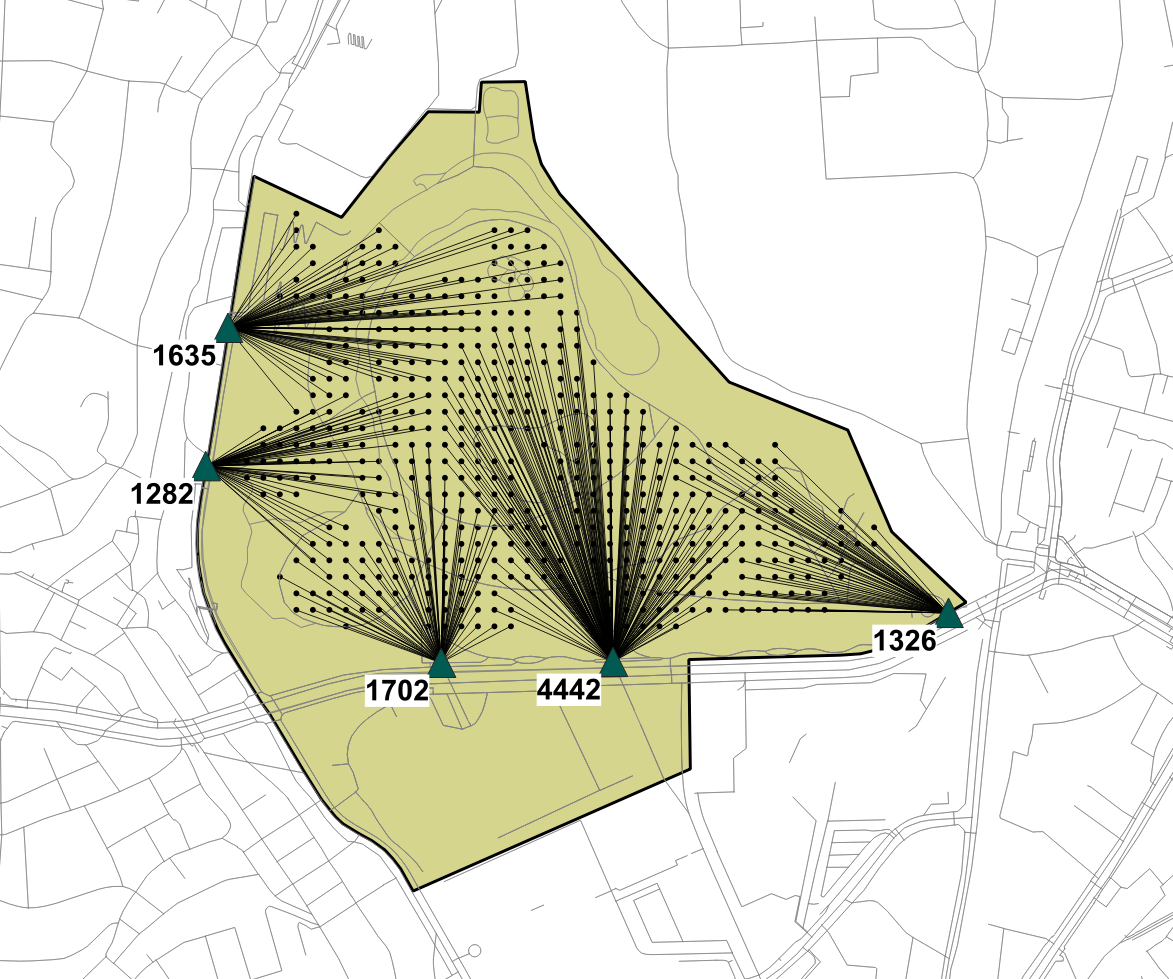
\includegraphics[width=\linewidth]{images/network/yoyogi_gatherings_nearest.png}\par\hspace{3pt}
    \par\captionof{figure}[Gatherings to closest entries]{Top to bottom: Hyde Park, Prospect Park, and Yoyogi Park. Number of gathering circles by closest entry point.}
    \label{fig:nearest_gatherings}
\end{minipage}

The gathering circles located and quantified in Chapter \ref{chapter_04} represent a physical space for one to four households---or one to four individuals---to hold a social activity outdoors. Therefore, the ideal ratio of residents to gathering circles is roughly one gathering circle for every four residents. Table \ref{table:all_pop_gath} shows the distribution of approximate population and gathering circles closest to each entry point. The population to gathering ratio ("Pop. to gath." column) divides the approximate population by the number of gathering circles associated with the same entry point. A value of one to four is ideal because it means there is one gathering circle for each resident up to one circle for every four residents. A value of zero implies that there are gathering circles associated with an entry point but no residents live closest to that entry. Any value greater than four and up to a value of "NaN" is indicative of more nearby residents than gathering circles, meaning there is likely an insufficient number of gathering circles for the surrounding population.

Figure \ref{fig:scatter_gath_pop} compares the distribution of the approximate population and number of gathering circles for each entry point at each park. Notable outliers for Prospect Park include entry point \#14 and entry point \#16, both of which have approximated populations exceeding 19,000, significantly higher than any other points at Prospect Park and also within Yoyogi Park and Hyde Park. In fact, entry point \#16 has a population to gathering ratio of nearly 278, meaning that for every gathering circle there are 278 residents living nearby. One explanation for these high values is that both entry points are adjacent to a stretch of park perimeter with few other entry points. Adding new entry points might decrease the number of residents that are currently closest to entry points \#14 and \#16. On the contrary, the outliers for Yoyogi Park (\#2) and Hyde Park (\#10) both have high quantities of gathering circles to low population approximations for the associated entry points, so the number of gatherings opportunities greatly surpasses the number of residents living within one-kilometer network distance. 

Further, Table \ref{table:avg_pop_gath} shows the population, gathering circles, population to gathering ratio, and food amenities (see the next section) averaged across the total number of entry points for each park. Hyde Park appears to have the best ratio of gathering circles to surrounding population with almost one circle for every person. Prospect Park has the least desirable ratio of one gathering circle for every nine people living nearby, and Yoyogi Park has one gathering circle for every three people. Depending on the weather conditions, for both Hyde Park and Yoyogi Park it is likely that there are enough gathering circles for everyone living within one-kilometer network distance to make use of one circle in groups of about four people. For Prospect Park, on the other hand, there are not enough social gathering circles for the surrounding population.

\end{multicols}

\begin{figure}[H]
  \centering
  \vspace{8pt}
  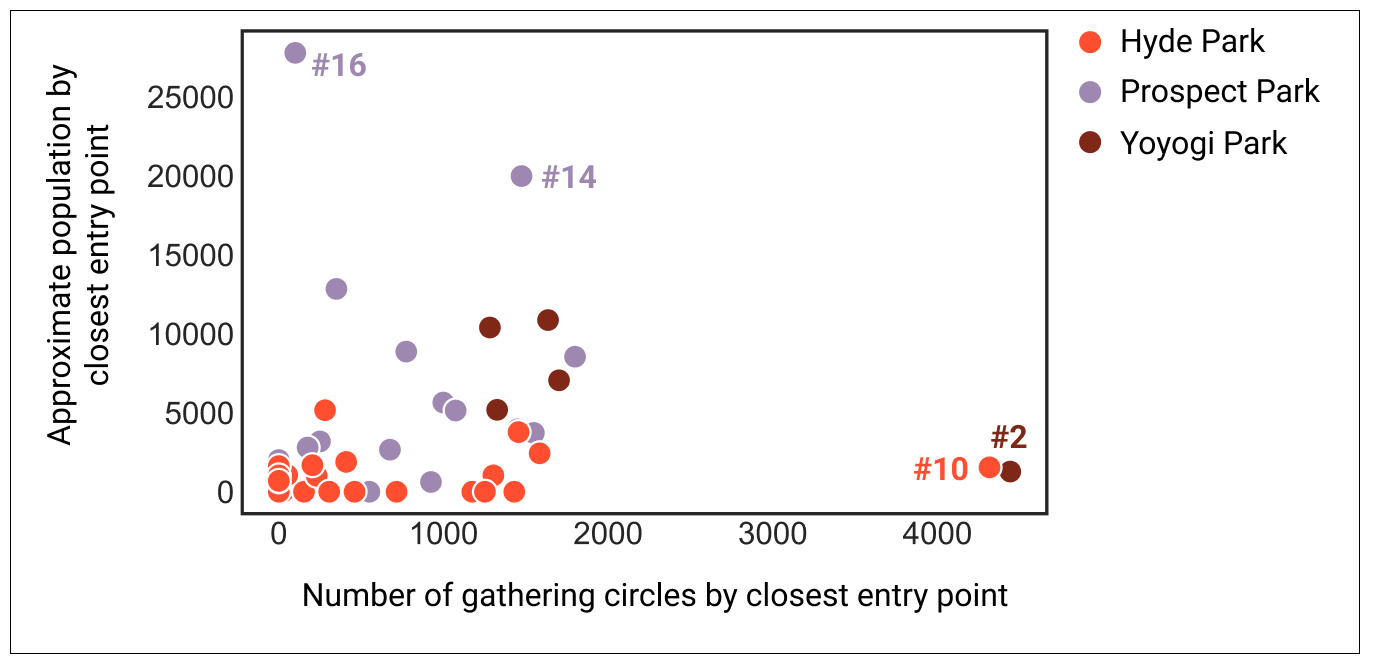
\includegraphics[width=0.9\textwidth]{images/network/scatter_pop_gath.png}
  \captionsetup{width=0.9\linewidth}
  \caption[Scatter plot]{Gathering circles and approximate population by entry point.}
  \label{fig:scatter_gath_pop}
\end{figure}\par

\begin{table}[H]
\centering
\small
\begin{tabular}{lcrrrrr}
\toprule
Park name &  Entry ID &  Approx. pop. &  Gatherings &  Pop. to gath. & Food (all) & Food (nearest) \\
\midrule
Hyde Park &         1 &           0 &        26 &      0.00 &       209 &             0 \\
{} &         2 &        1889 &       409 &      4.62 &       276 &           115 \\
{} &         3 &           0 &       715 &      0.00 &       253 &            30 \\
{} &         4 &        5162 &       281 &     18.37 &       247 &           115 \\
{} &         5 &           0 &      1175 &      0.00 &       292 &            10 \\
{} &         6 &        3775 &      1456 &      2.59 &       278 &            98 \\
{} &         7 &        2435 &      1584 &      1.54 &       297 &            28 \\
{} &         8 &           0 &         0 &       NaN &       281 &             9 \\
{} &         9 &           0 &      1430 &      0.00 &       280 &            36 \\
{} &        10 &        1544 &      4316 &      0.36 &       253 &             2 \\
{} &        11 &           0 &      1175 &      0.00 &       234 &             0 \\
{} &        12 &        1053 &        51 &     20.65 &       202 &           106 \\
{} &        13 &           0 &         0 &       NaN &       205 &             4 \\
{} &        14 &         661 &         0 &       NaN &       193 &            11 \\
{} &        15 &           0 &       460 &      0.00 &       182 &             0 \\
{} &        16 &        1037 &      1303 &      0.80 &       154 &            39 \\
{} &        17 &        1624 &         0 &       NaN &       144 &            21 \\
{} &        18 &           0 &       153 &      0.00 &       133 &            44 \\
{} &        19 &        1011 &       230 &      4.40 &       115 &            19 \\
{} &        20 &        1034 &         0 &       NaN &       111 &             0 \\
{} &        21 &         690 &         0 &       NaN &        65 &            26 \\
{} &        22 &        1681 &       204 &      8.24 &        36 &             0 \\
{} &        23 &           0 &       306 &      0.00 &        39 &             4 \\
{} &        24 &           0 &      1252 &      0.00 &        42 &             1 \\
\midrule
Prospect Park &         1 &         618 &       924 &      0.67 &        94 &             0 \\
{} &         2 &        5649 &       999 &      5.65 &       131 &            24 \\
{} &         3 &        5143 &      1074 &      4.79 &       150 &            29 \\
{} &         4 &        1859 &         0 &       NaN &        21 &             5 \\
{} &         5 &        2661 &       675 &      3.94 &        43 &            11 \\
{} &         6 &           0 &       550 &      0.00 &        55 &             2 \\
{} &         7 &        3185 &       250 &     12.74 &       140 &            36 \\
{} &         8 &        2005 &         0 &       NaN &       156 &             0 \\
{} &         9 &        8872 &       774 &     11.46 &       108 &            35 \\
{} &        10 &        3948 &      1449 &      2.72 &       121 &            15 \\
{} &        11 &        8548 &      1799 &      4.75 &       126 &            44 \\
{} &        12 &         430 &         0 &       NaN &        24 &             1 \\
{} &        13 &        2798 &       175 &     15.99 &        59 &             2 \\
{} &        14 &       19984 &      1474 &     13.56 &       160 &           131 \\
{} &        15 &        3722 &      1549 &      2.40 &       100 &            14 \\
{} &        16 &       27783 &       100 &    277.83 &       162 &           117 \\
{} &        17 &       12841 &       350 &     36.69 &       132 &            71 \\
\midrule
Yoyogi Park &         1 &        5187 &      1326 &      3.91 &       342 &           271 \\
{} &         2 &        1278 &      4442 &      0.29 &       390 &           142 \\
{} &         3 &        7056 &      1702 &      4.15 &       172 &            53 \\
{} &         4 &       10396 &      1282 &      8.11 &       103 &            48 \\
{} &         5 &       10869 &      1635 &      6.65 &        91 &            21 \\
\bottomrule
\end{tabular}
\caption[Approximate population to gatherings]{Approximate population and number of gathering circles to the closest entry points.}
\label{table:all_pop_gath}
\end{table}

\begin{table}[H]
\centering
\small
\begin{tabular}{lcrrrrr}
\toprule
{}     & Entry ID &  Approx pop. &  Gatherings &  Pop. to gath. &  Food (all) &  Food (nearest) \\
Park name &  \textit{(count)} &  \textit{(avg.)} &  \textit{(avg.)} &  \textit{(avg.)} &  \textit{(avg.)} &  \textit{(avg.)} \\
\midrule
Hyde Park     &        24 &         983 &       689 &      1.43 &       188 &            30 \\
Prospect Park &        17 &        6473 &       714 &      9.06 &       105 &            32 \\
Yoyogi Park   &         5 &        6957 &      2077 &      3.35 &       220 &           107 \\
\bottomrule
\end{tabular}
\caption[Entry point averages]{Average population and number of gathering circles by entry point for each park.}
\label{table:avg_pop_gath}
\end{table}

\begin{multicols}{2}
    
\subsection{Reach of food amenities}
A \textit{Reach} value is also calculated from individual park entry points to the food amenities within the one-kilometer network distance from the gathering circles. As mentioned previously, the time and distance required to leave a social gathering in a park in order to retrieve food and return is usually prohibitively inconvenient, which is why many picnickers procure food in advance of arriving at the park. This section of the research will compare the access to food for social gatherings across the three parks to see which park provides the most food amenities that could be utilized in combination with social gatherings in parks.

For the purpose of this study, all food-related amenities---restaurants, cafes, bars, grocery stores, convenience stores, etc.---are included as options for procuring food for social gatherings. When COVID-19 began, many facilities closed for indoor dining and began offering only take-out services \cite{wang_adoption_2021}. In fact, because the duration of the public health crisis was unpredictable, New York City even allowed bars and restaurants to serve alcohol for takeout and delivery to keep such amenities in business \cite{del_castillo_covid_2020}. The data for food facilities is gathered through the OpenStreetMaps plug-in for QGIS, using "Facilities/Food+Drinks" and "Shops/Food" as the keyword search criteria. The tool compiles geographic point data for restaurants, cafes, bars, grocery and convenience stores, and specialty markets. Then, this data is isolated to the convex hull created in Section \ref{approx_pop} representing a network distance of one-kilometer from gathering circles to the surrounding neighborhood, meaning the amenities in question are all located between the boundary of the approximated population and the park entry points.

\end{multicols}

\begin{figure}[H]
  \centering
  \vspace{8pt}
  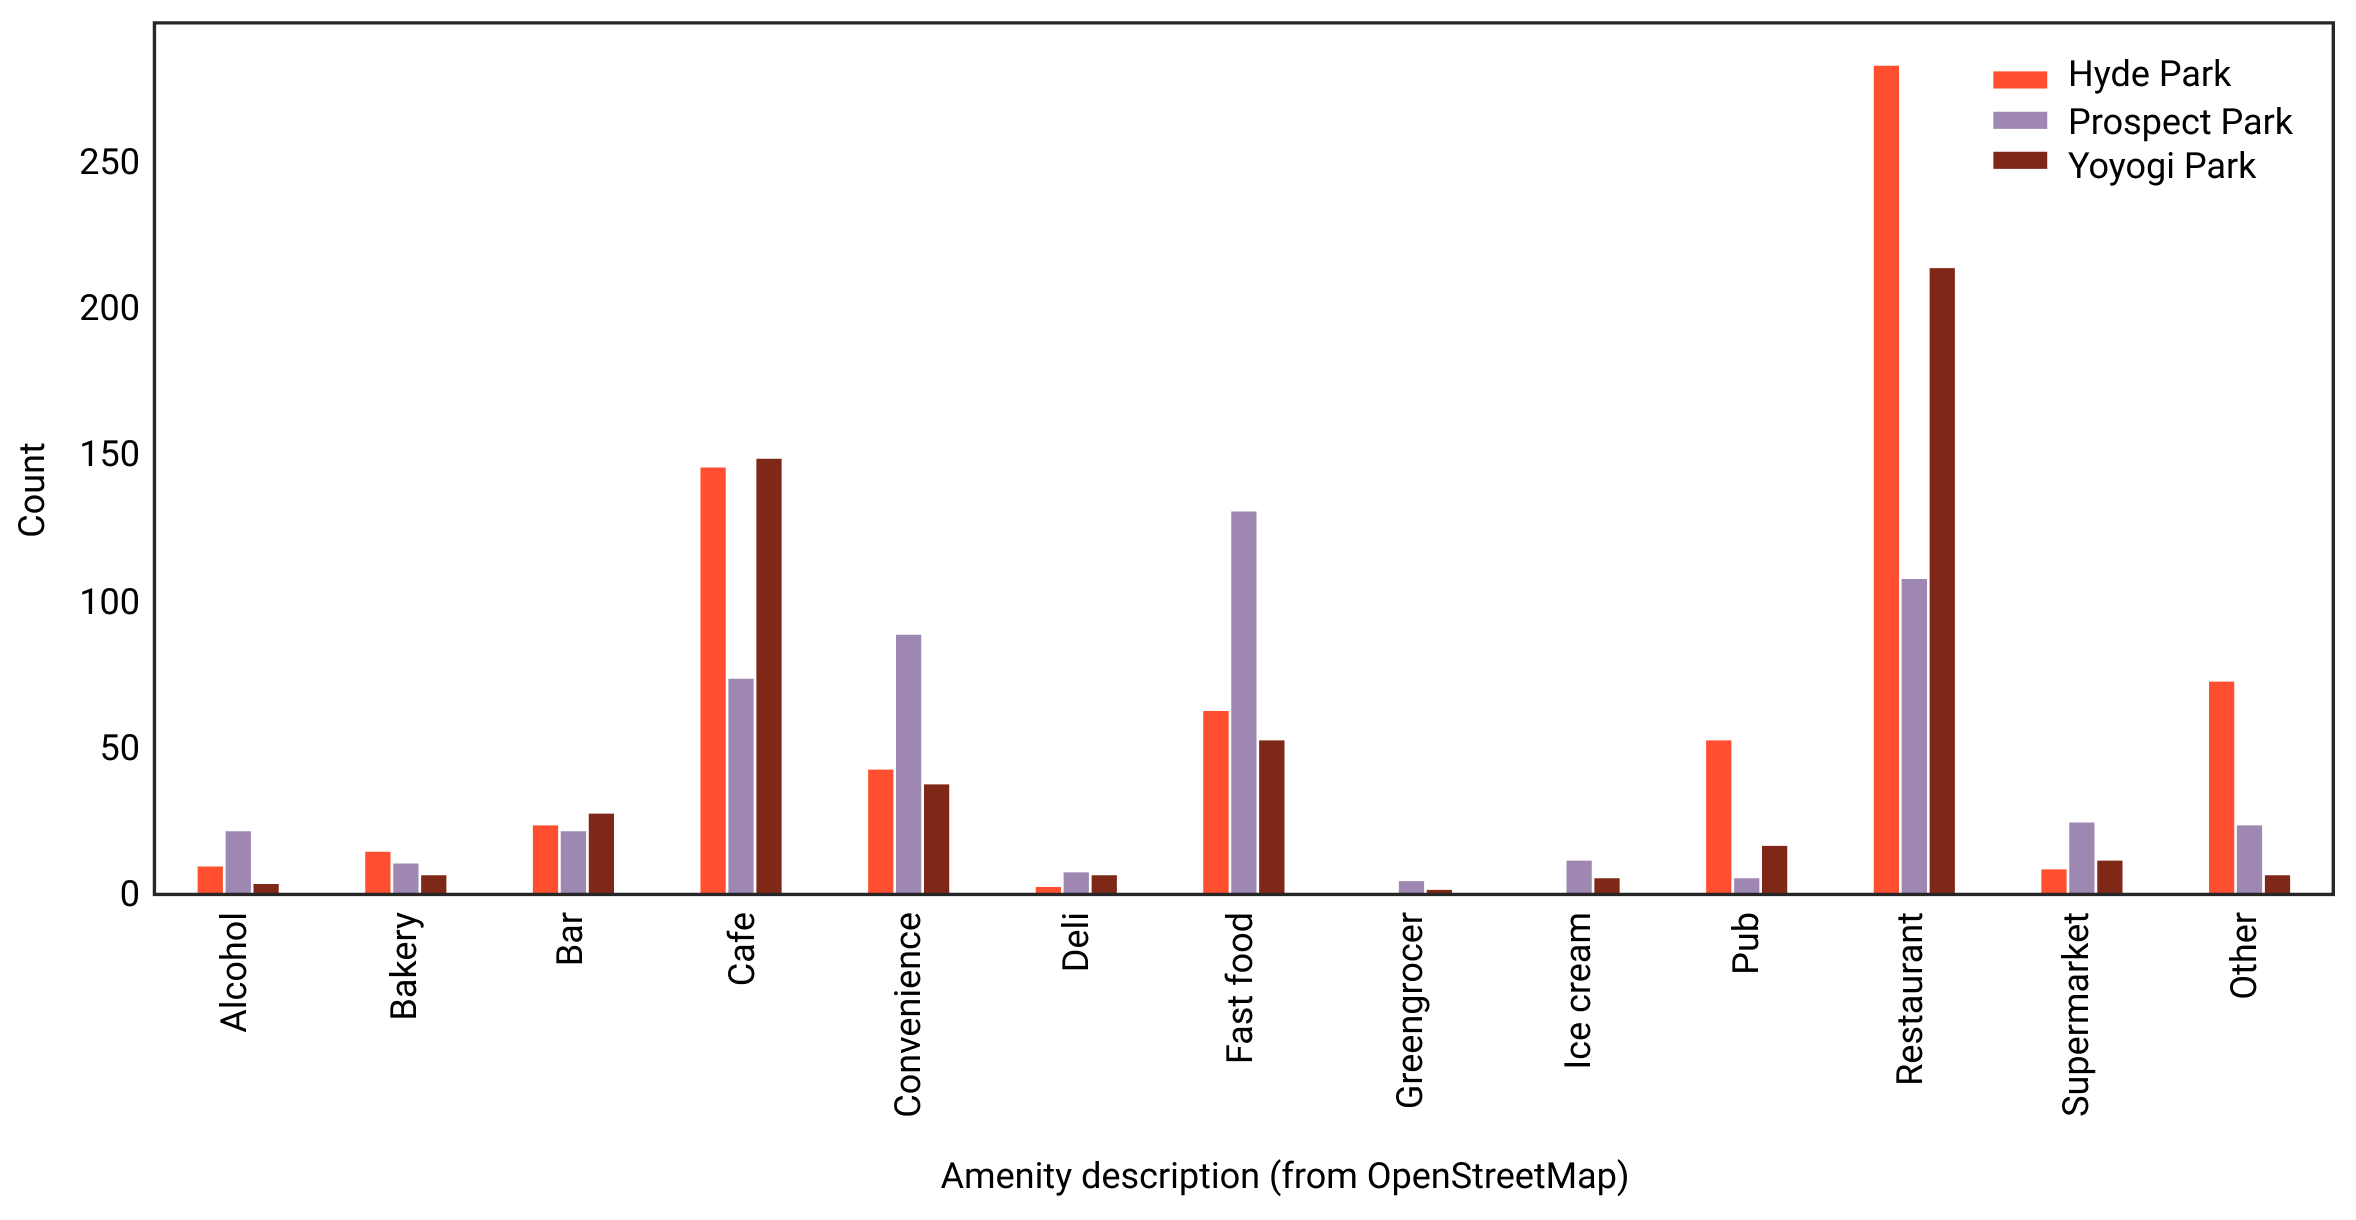
\includegraphics[width=1.0\textwidth]{images/network/amenity_bar_chart.png}
  \captionsetup{width=1.0\linewidth}
  \caption[Bar plot]{Amenities within 1-km network distance of gathering circles.}
  \label{fig:amenity_bar_chart}
\end{figure}\par

\begin{multicols}{2}

Figure \ref{fig:amenity_bar_chart} is a grouped bar chart for Hyde Park, Prospect Park and Yoyogi Park, with the quantities of the amenities classified in OpenStreetMaps. Despite the varying sizes of the parks in question, with Prospect Park the largest at 1.8 square kilometers, Yoyogi Park and Hyde Park have far more restaurants within one-kilometer network distance of the social gathering circles (over 200 compared to Prospect Park's 100). The number of cafes shows a similar discrepancy, with only convenience stores and fast food restaurants around Prospect Park outnumbering those of Hyde Park and Yoyogi Park. Interestingly, specialty markets and grocery stores are similarly few in quantity across the three parks.

Next, reach values are determined from the entry points to the nearby food amenities (see Table \ref{table:all_pop_gath} for values by entry point and Table \ref{table:avg_pop_gath} for average values by park). Figure \ref{fig:scatterplots} visualizes the food amenities compared to the approximate population and the gathering circles respectively. In the population scatter plot, most of the reach values are in the range of 50 or less food amenities to less than 10,000 residents, but each park has several outlier entry points. The two entry points to Prospect Park found to be nearest to more than 19,000 residents (\#14 and \#16) each have less than 150 food amenities that are also nearest to those entry points. An outlier for Yoyogi Park (\#1), on the other hand, has one entry point with over 250 closest food shops and an approximate population of less than 5000 residents, indicating the presence of a highly commercialized zone.

\end{multicols}

\begin{figure}[H]
  \centering
  \vspace{8pt}
  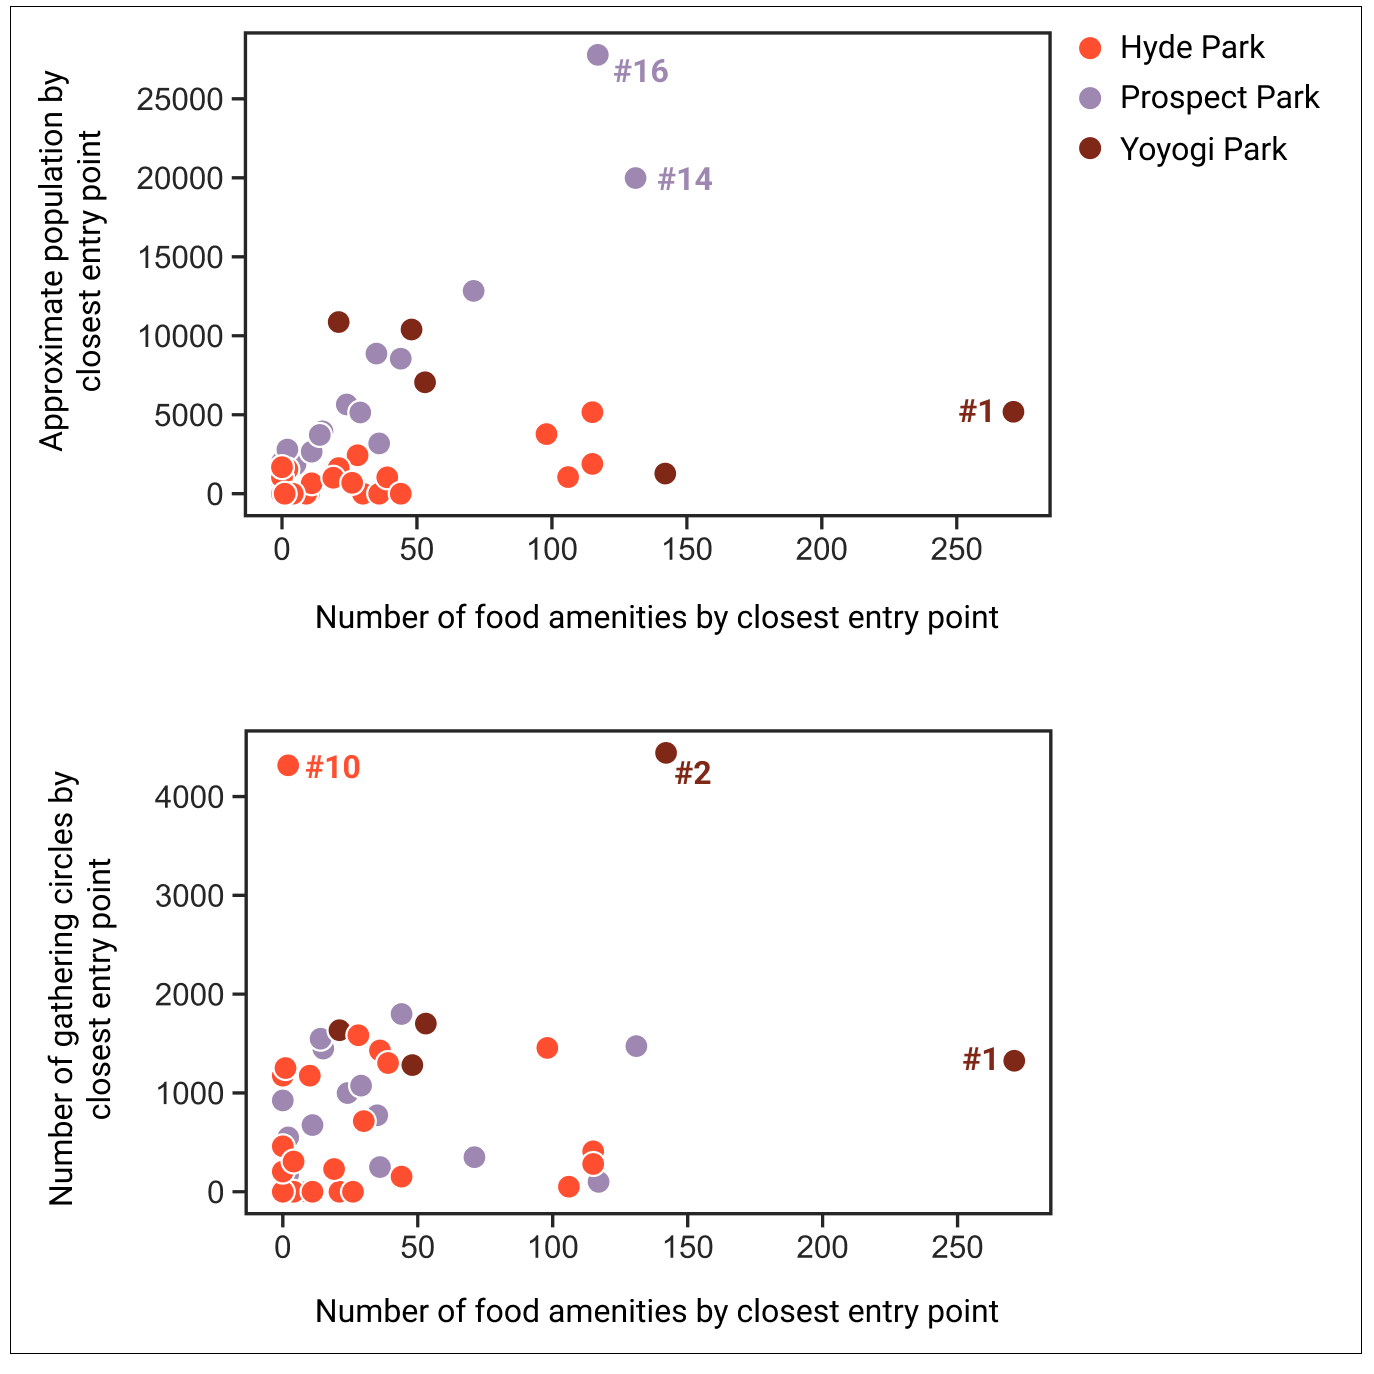
\includegraphics[width=0.9\textwidth]{images/network/scatterplots.png}
  \captionsetup{width=0.9\linewidth}
  \caption[Scatter plots]{Food amenities by gathering circles and approximate population by entry point.}
  \label{fig:scatterplots}
\end{figure}\par

\begin{multicols}{2}

When comparing the number of food amenities to the number of gathering circles closest to each entry point, some of the same outliers are evident. Again, entry point \#1 to Yoyogi Park has over 250 food amenities but does not have as many gathering circles as entry point \#2, with over 4000 gathering circles and less than 150 food amenities. This is exemplary of how \#2, which is also not near many residents as explained above, is an entry point near the large commercial and transportation hub of Shibuya. This makes social gatherings during non-pandemic times accessible for out-of-neighborhood visitors who are picking up food, but it means that the majority of food nearest to the park is not nearest to the residents. Similarly, Hyde Park has more than 4000 gathering circles closest to entry point \#10 but only two food amenities are closest to that entry point. Visitors using this entry to get to a gathering circle therefore might have fewer options for food. One caveat to this analysis is that while only two amenities are \textit{closest} to that entry point, when calculating all food amenities less than one-kilometer network distance from the entry point, more than 250 amenities are within reach---see the "Food (all)" column of Table \ref{table:all_pop_gath}. 

From the perspective of the gathering circles, Figures \ref{fig:hyde_reach} - \ref{fig:yoyogi_reach} show the reach values for the number of restaurants (in intervals of 50, see Figure \ref{fig:reach_legend}) within one-kilometer network distance of each gathering circle, with the previously found approximate populations labelled at each entry point. 

Overall Prospect Park has the least number of social gathering circles that are within a one-kilometer walk of food amenities as seen in Figure \ref{fig:prospect_reach}. This is due to both the positioning of the gathering circles largely in the center of the park, as well as because the food amenities located northwest of the park are concentrated on one street that is two blocks away from the park border. On the other hand, Hyde Park (Figure \ref{fig:hyde_reach}) has more equally spaced entry points and many food amenities throughout the neighborhood, meaning the gathering circles which are not in the center of the park or near the west side adjacent to Kensington Gardens, generally have access to more than 100 food amenities within a one-kilometer walk. The entries to Yoyogi Park which have the largest approximate populations labeled on Figure \ref{fig:yoyogi_reach} are west of the park whereas the gathering circles which have reach values of more than 200 food amenities are east and south. This is an uneven distribution of amenities from the perspective of pandemic conditions when commercial areas are not being used in the same way they are in non-pandemic times, and those amenities could better serve people living nearby. Therefore, despite having the lowest average "Food (nearest)" reach value in Table \ref{table:avg_pop_gath}, Hyde Park has the most evenly distributed population and food amenity access based on the findings of this reach value analysis.

\begin{figure}[H]
  \centering
  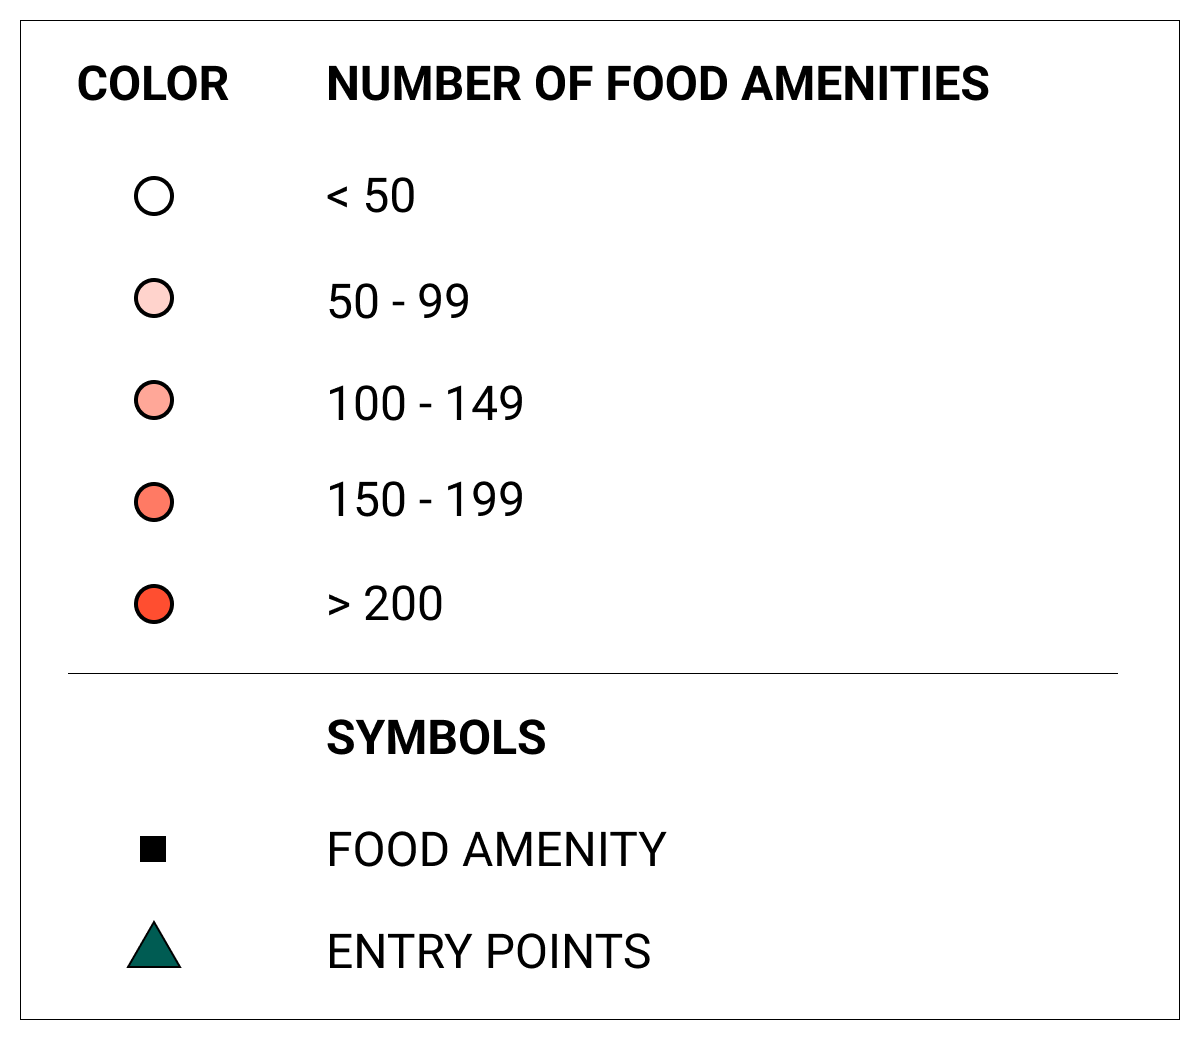
\includegraphics[width=0.45\textwidth]{images/network/reach_legend.png}\par\captionof{figure}[Reach legend]{Food amenity reach analysis legend.}
  \label{fig:reach_legend}
\end{figure} 

\end{multicols}

\begin{figure}[H]
  \centering
  \captionsetup{width=0.9\textwidth}
  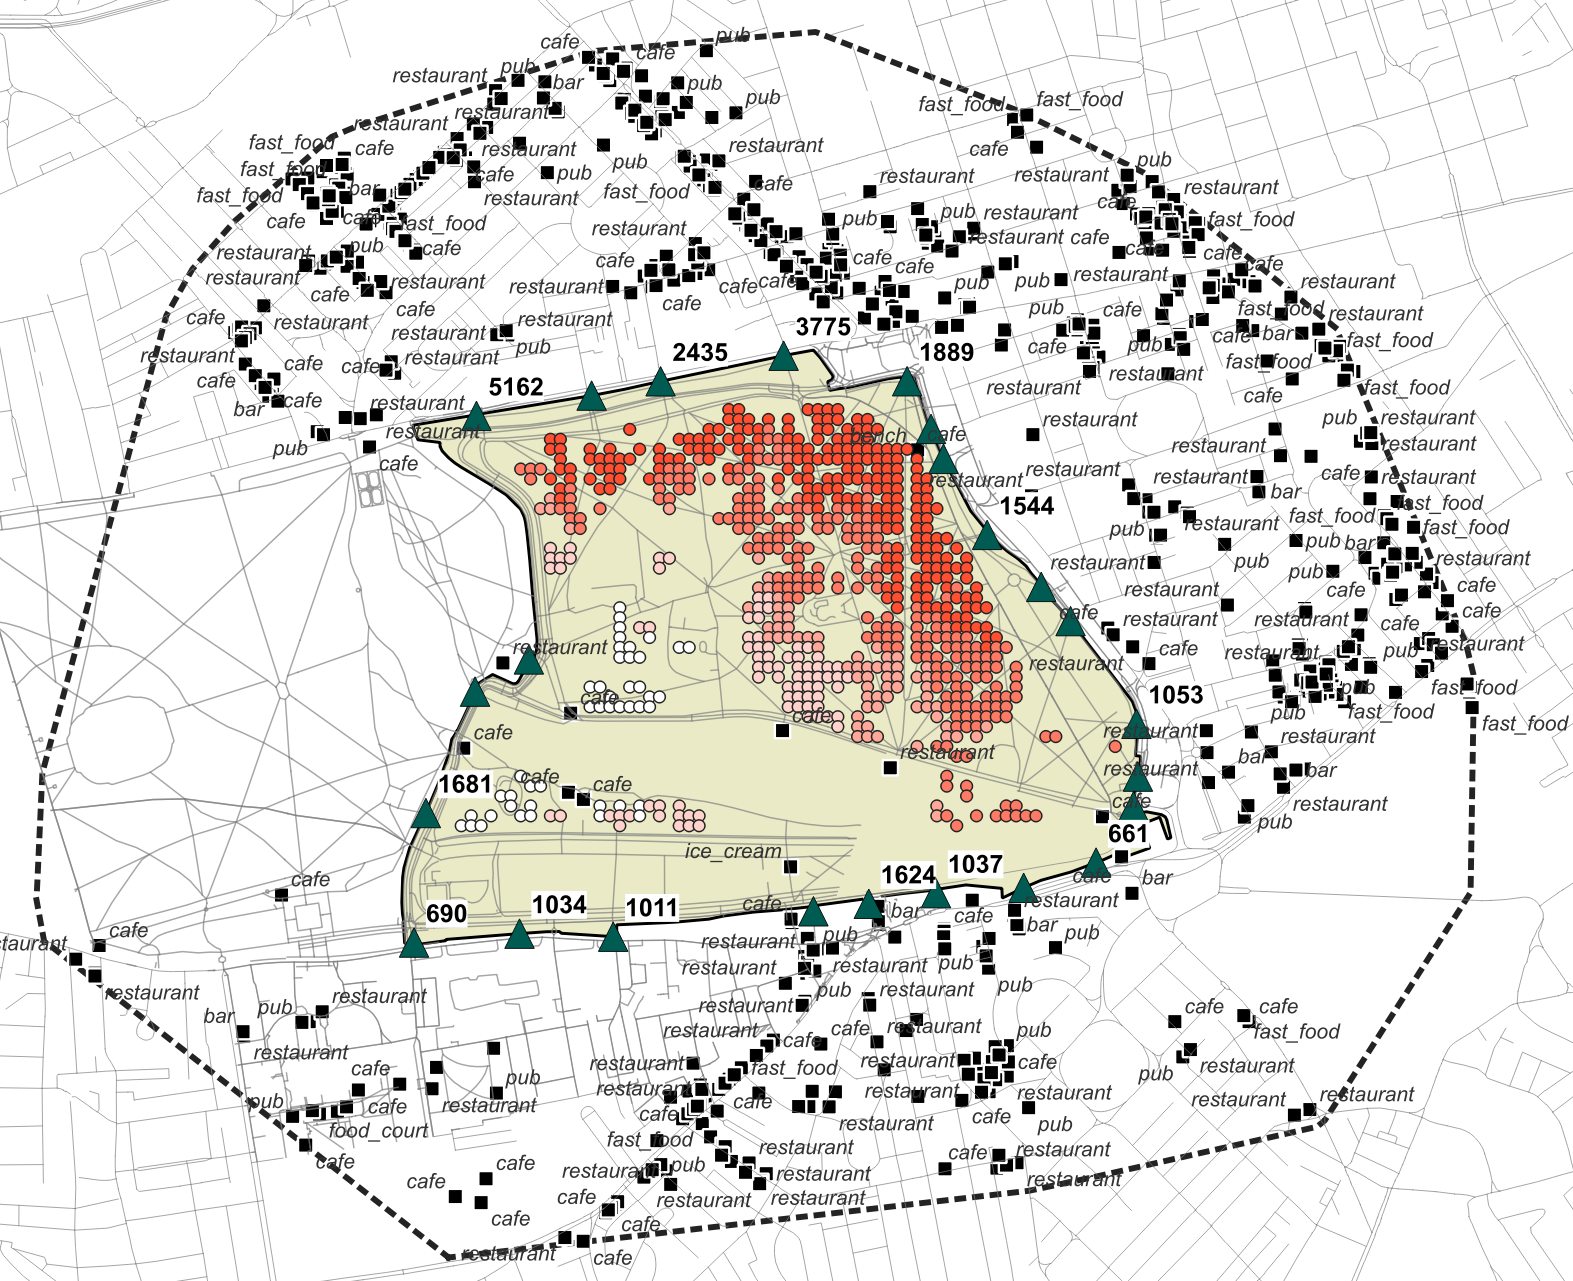
\includegraphics[width=0.75\textwidth]{images/network/hyde_gath_food_pop.png} \\
  \caption[Hyde Park - reach]{Food, population and gatherings combined reach analysis for Hyde Park.}
  \label{fig:hyde_reach}
\end{figure}

\begin{figure}[H]
  \centering
  \captionsetup{width=0.9\textwidth}
  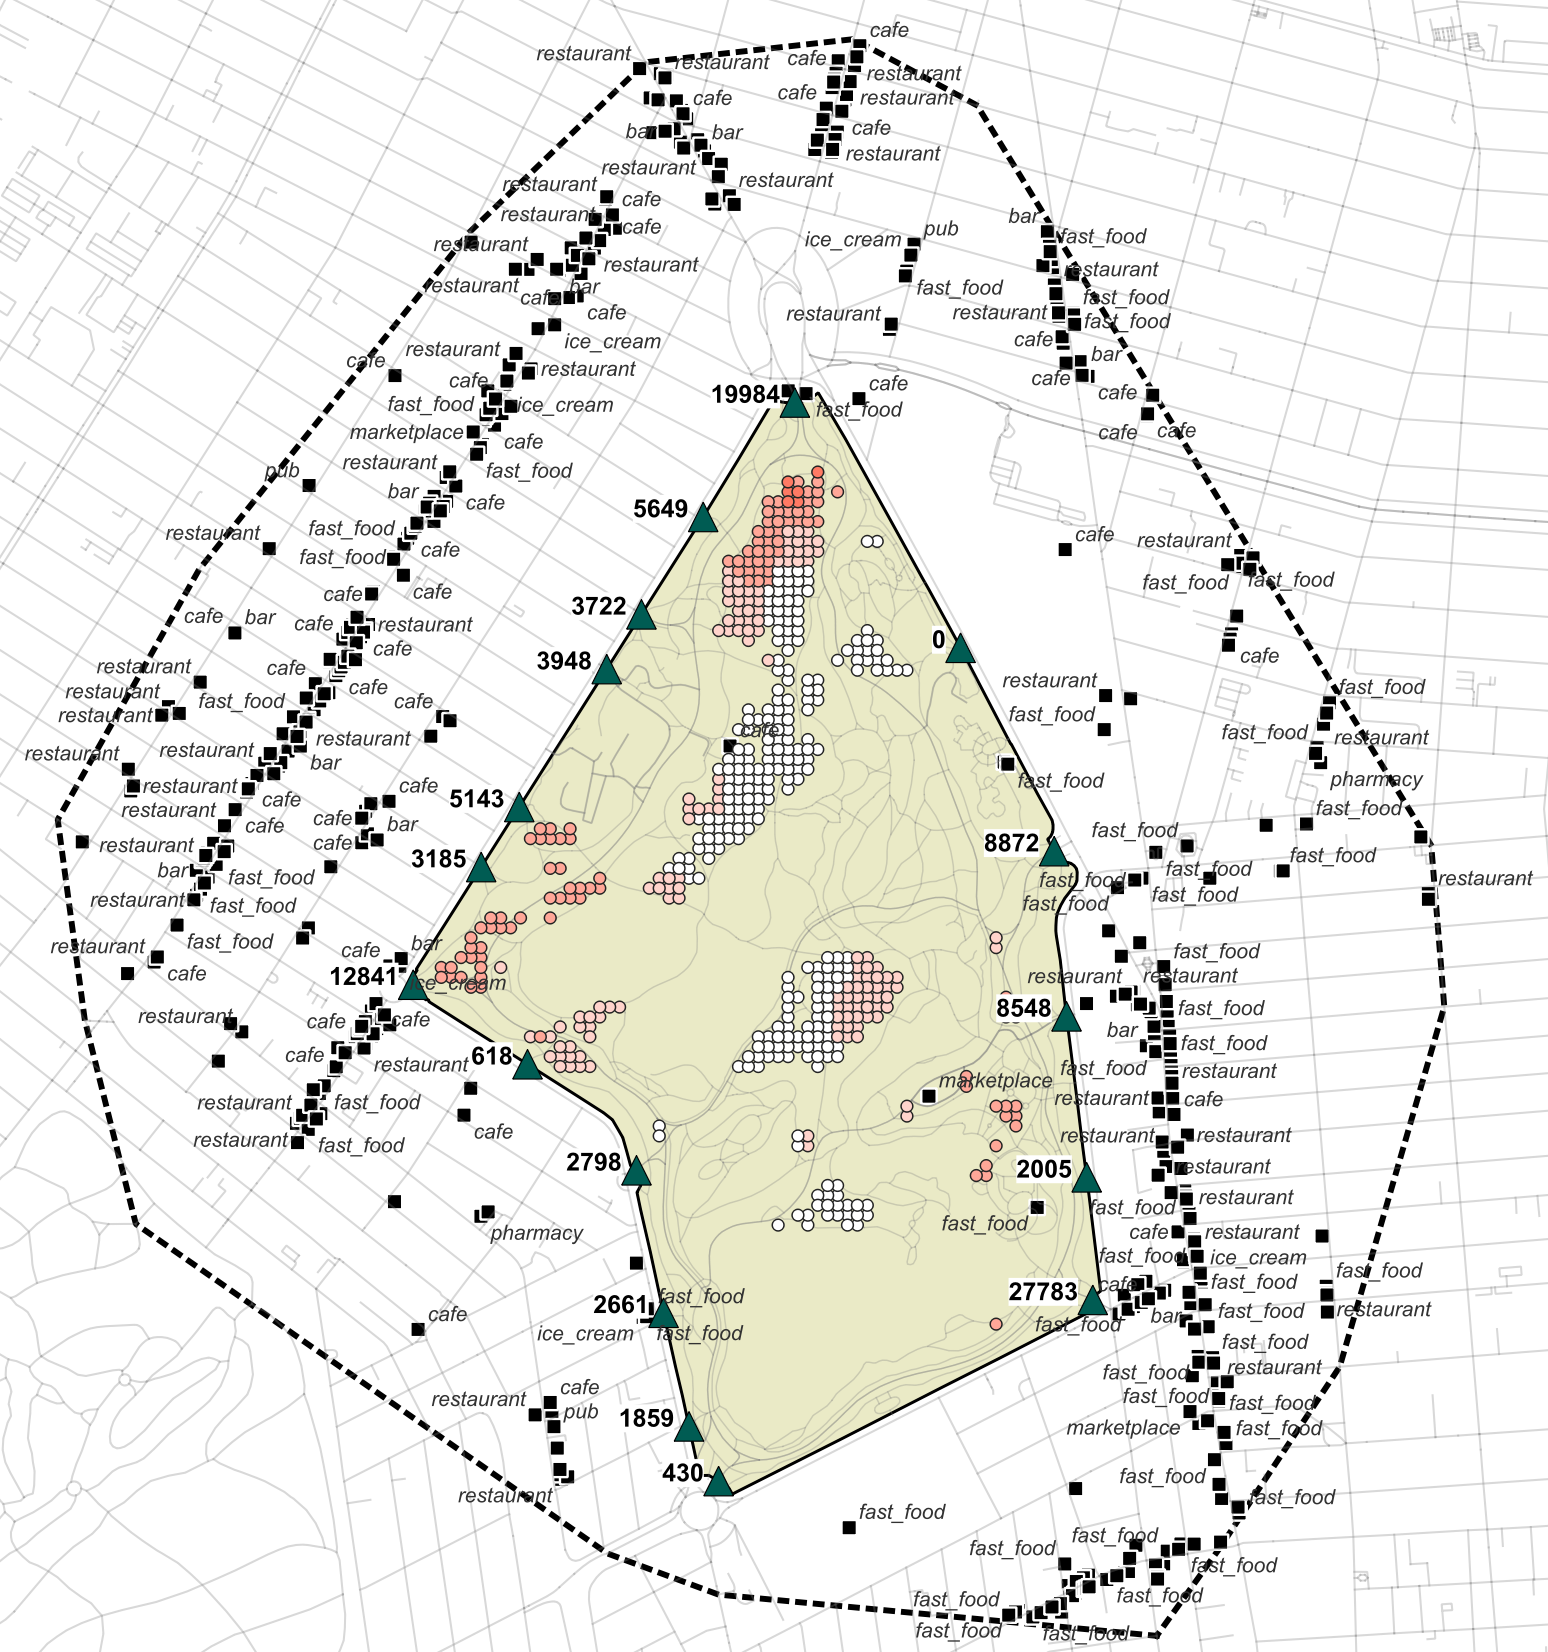
\includegraphics[width=0.75\textwidth]{images/network/prospect_gath_food_pop.png} \\
  \caption[Prospect Park - reach]{Food, population and gatherings combined reach analysis for Prospect Park.}
  \label{fig:prospect_reach}
\end{figure}

\begin{figure}[H]
  \centering
  \captionsetup{width=0.9\textwidth}
  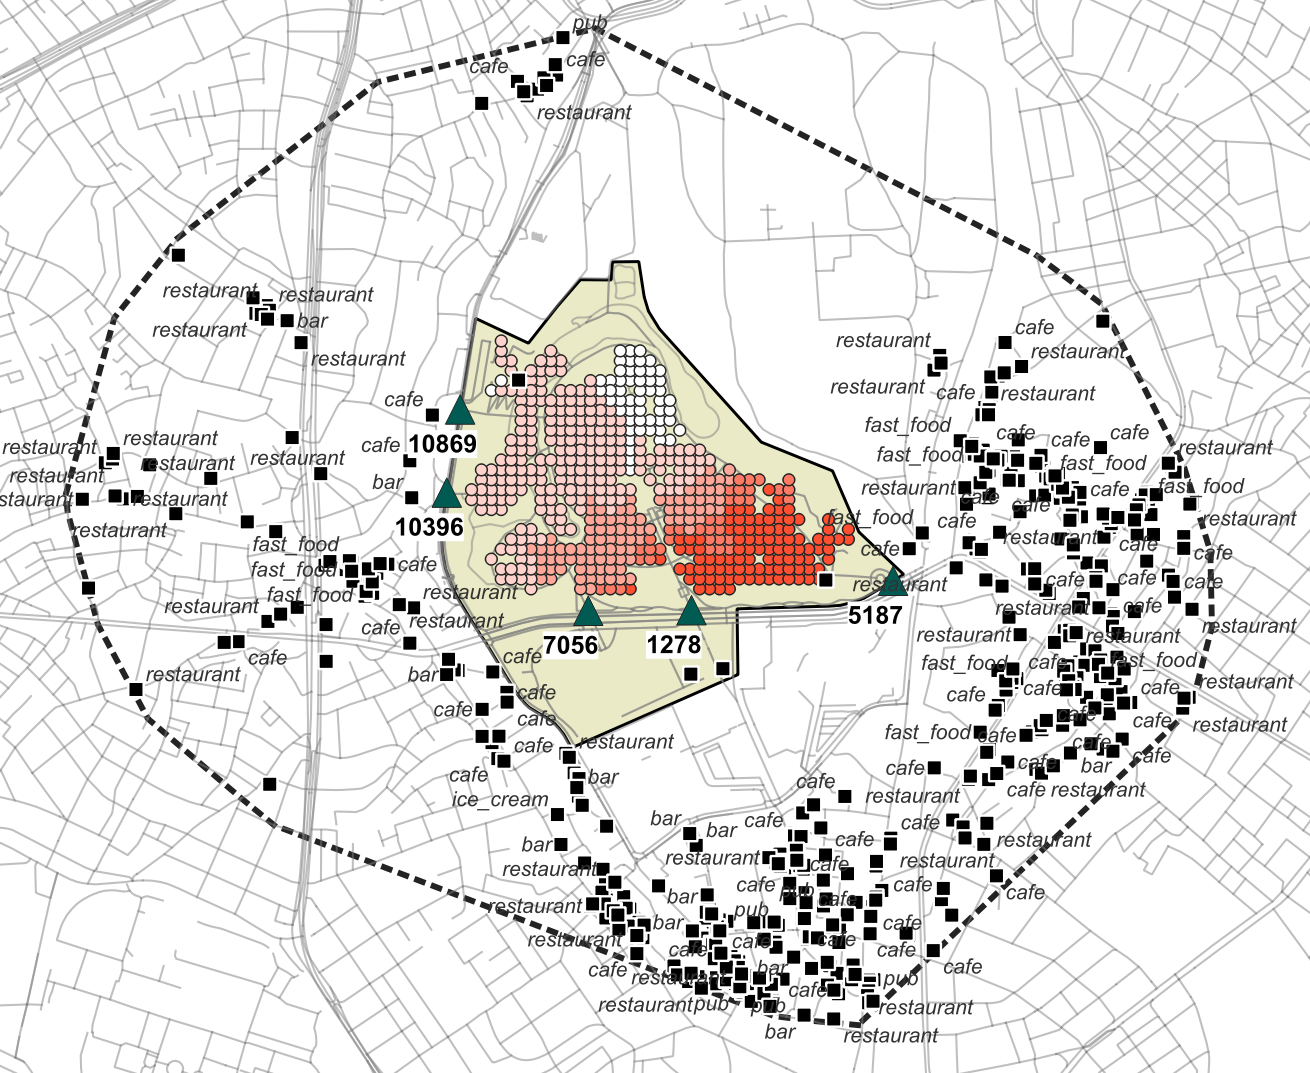
\includegraphics[width=0.8\textwidth]{images/network/yoyogi_gath_food_pop.png} \\
  \caption[Yoyogi Park - reach]{Food, population and gatherings combined reach analysis for Yoyogi Park.}
  \label{fig:yoyogi_reach}
\end{figure}

\begin{multicols}{2}

\section{Betweenness analysis}
\subsection{Observer points}
The \textit{Patronage betweeness} tool in the UNA toolbox counts how many trips from origin points to destination points pass observer points along the network \cite{sevtsuk_tale_2022}. This tool is used to estimate pedestrian traffic routes from the viewpoint of both the amenities that are passed along the way (the observer points) as well as the network edges traveled. The \textit{Betweenness} index used in the UNA toolbox is defined as:
\begin{multline}
        \textit{Betweenness}[\textit{i}]^{\textit{r,dr}} = \\
        \\
        \sum_{\textit{j,k}\in\textit{G}-\{\textit{i}\}.\textit{d}[\textit{j},\textit{k}]\le\textit{r}*\textit{dr}} \frac{n_\textit{j,k} [i]}{n_\textit{j,k}} * \textit{W}[\textit{j}] * \frac{1}{f(d[j,k])}\\
        \label{eqn:betweenness_eqn}
\end{multline}

Where \textit{Betweenness} $[i]^r,dr$ is the value summed at the observer points [\textit{i}] within the search radius \textit{r}, detour ratio \textit{dr}, $n_j,k[i]$ is the number of shortest paths that pass by the observer points, and $n_j,k$ is the number of the shortest paths from \textit{j} to \textit{k} \cite{sevtsuk_tale_2022}. The origin weight \textit{W[j]} is set to the approximate population of the intersection points, based on the population analysis completed in Section \ref{approx_pop}. The resulting betweenness index is the approximate number of neighboring residents that pass by each food amenity along the shortest distance walk from the intersection near home to the closest park entry point.

Some features of the \textit{Patronage Betweenness} tool are not utilized for this analysis, such as the \textit{Decay} feature, which predicts trips between the two points to be less likely when they are further away from each other \cite{sevtsuk_tale_2022}. This feature is not used because during a pandemic, a one-kilometer walk to a park is likely better access than the majority city residents; therefore, this analysis assumes that residents as far as one-kilometer benefit from park access during a pandemic, so it is feasible to assume the park is used for social activities for that population. 

\end{multicols}

\begin{figure}[H]
  \centering
  \captionsetup{width=0.9\textwidth}
  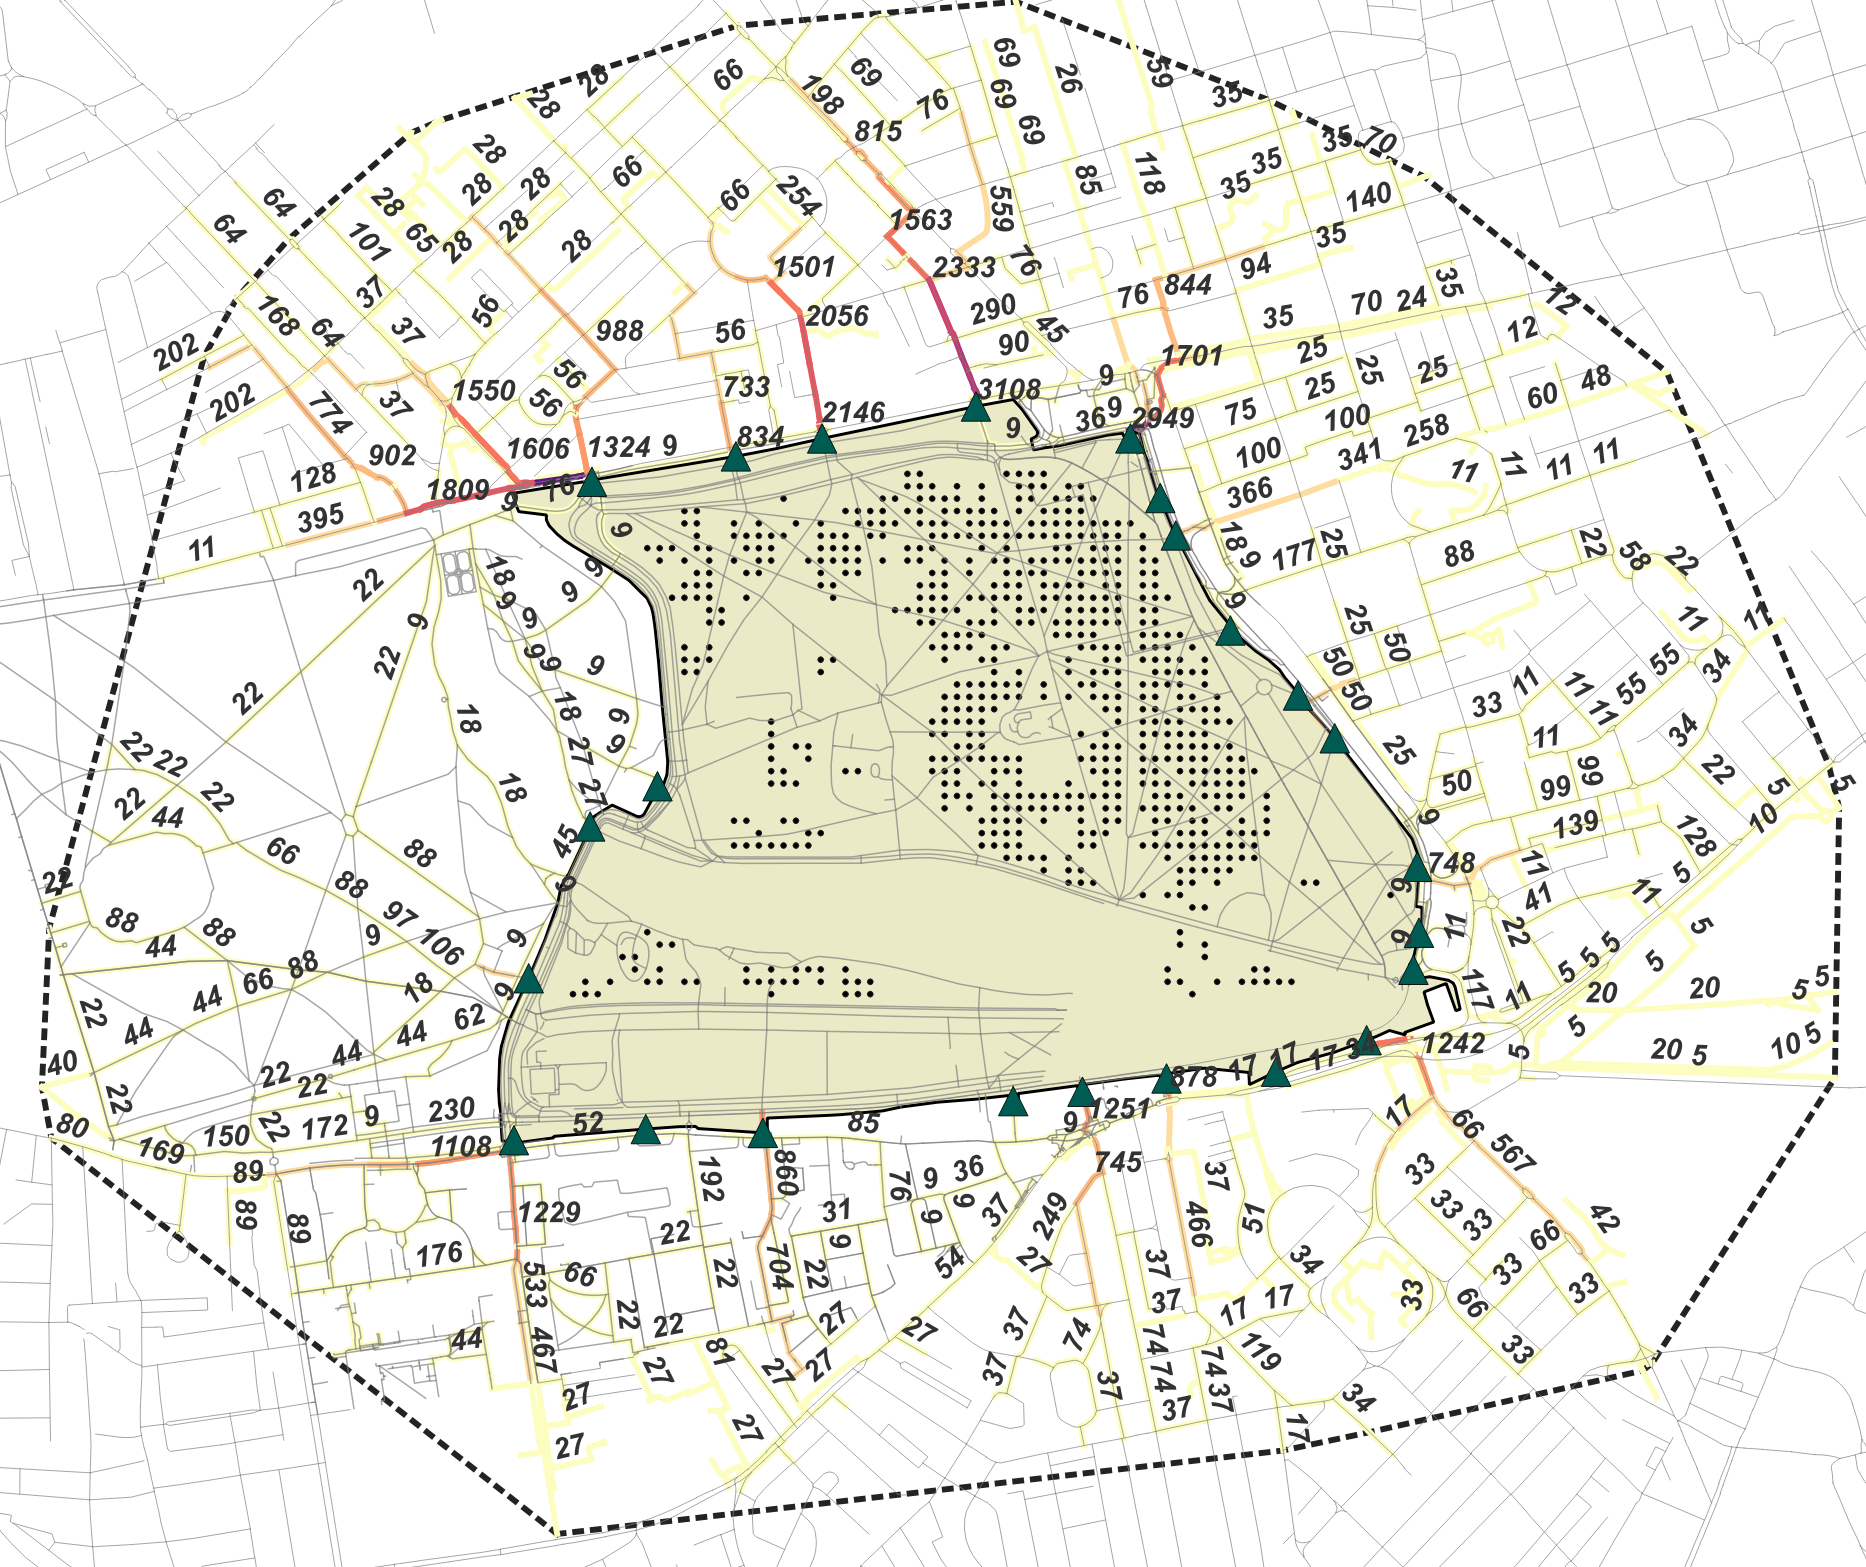
\includegraphics[width=0.9\textwidth]{images/network/hyde_betweenness_roads.png} \\
  \vspace{10pt} % Adjust vertical spacing between the images
  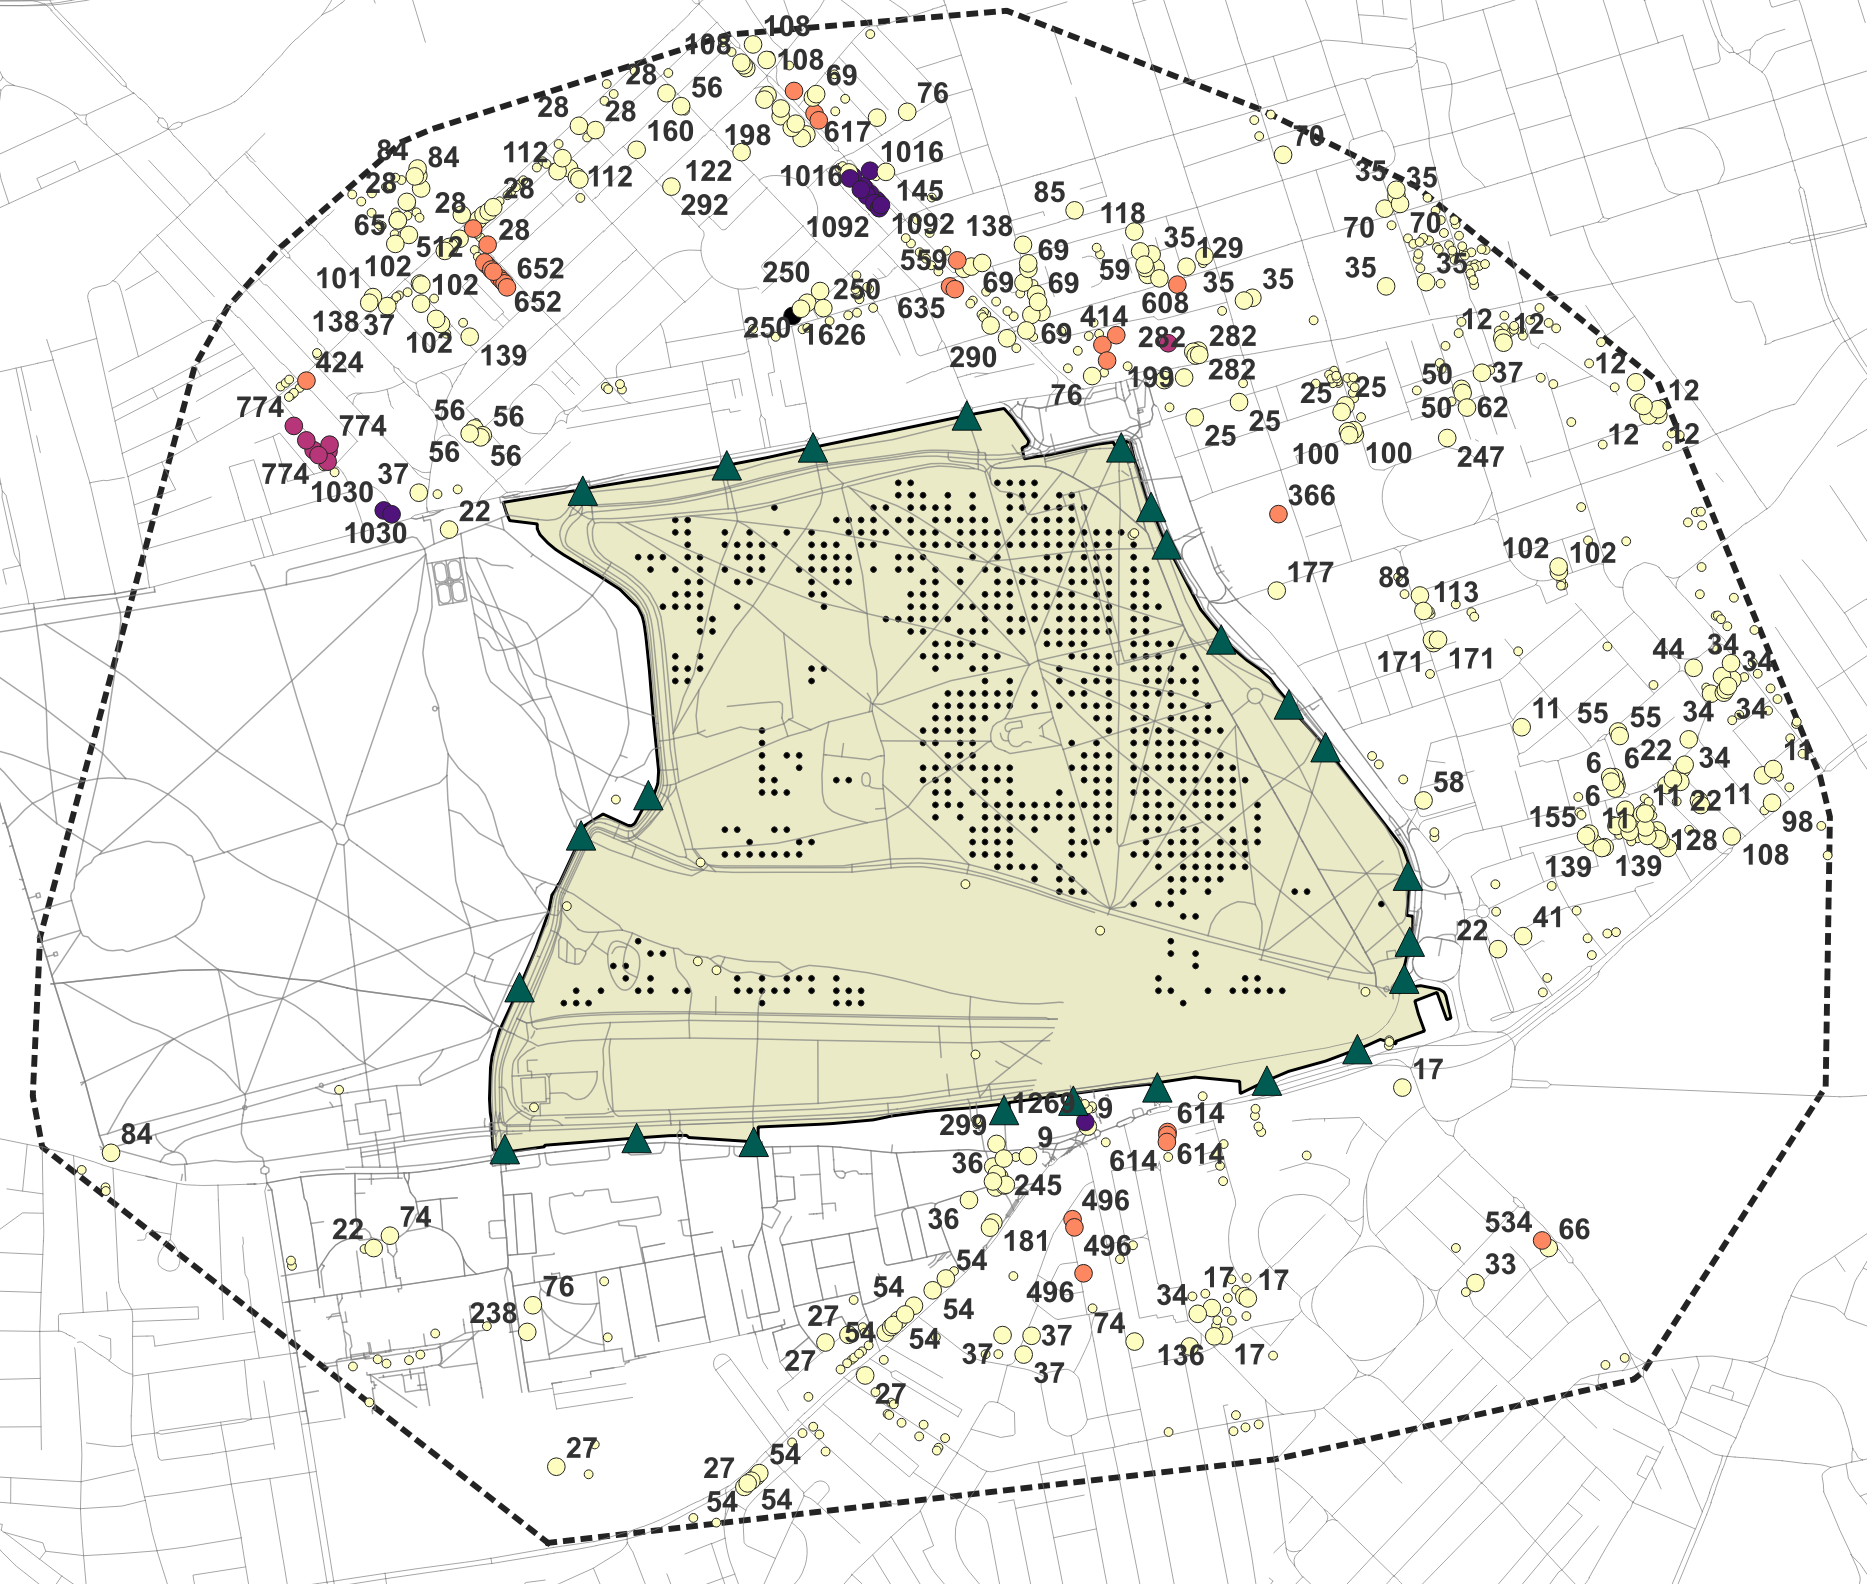
\includegraphics[width=0.9\textwidth]{images/network/hyde_betweenness_food.png} \\
  \vspace{10pt}
  \caption[Hyde Park - betweenness]{Betweenness results for network edges and food amenities surrounding Hyde Park.}
  \label{fig:hyde_betweenness}
\end{figure}

\newpage
\null
\vfill
\begin{figure}[H]
  \centering
  \captionsetup{width=0.8\textwidth}
  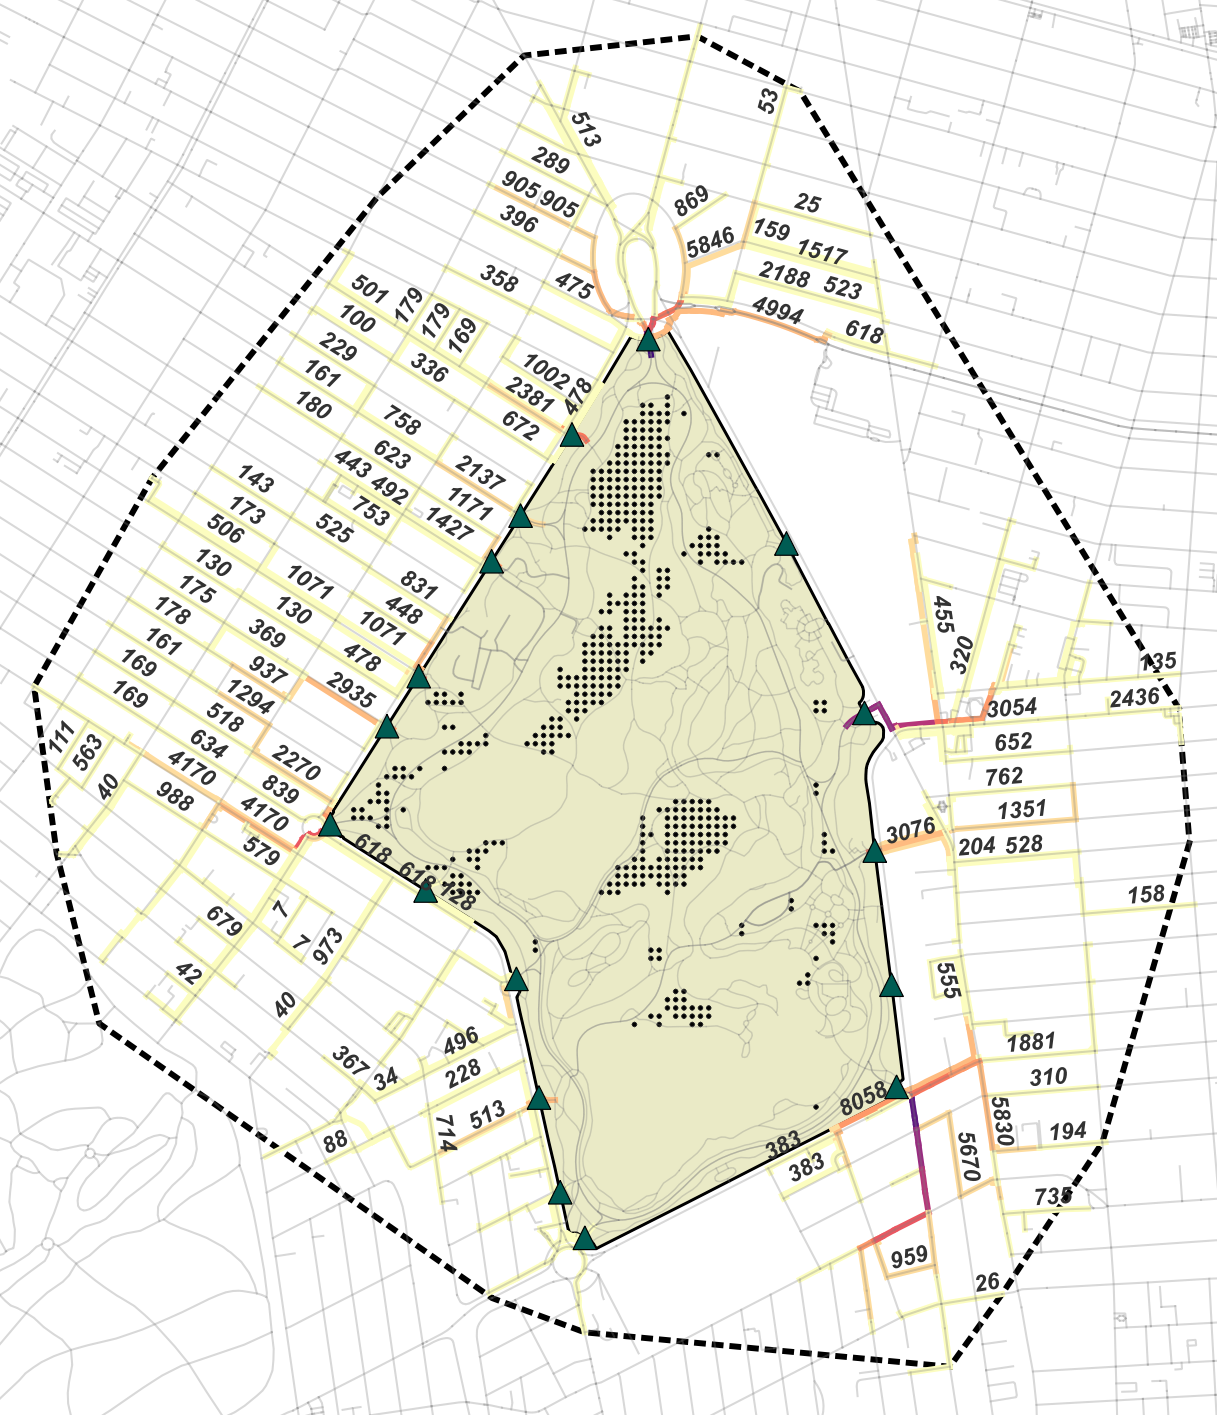
\includegraphics[width=0.8\textwidth]{images/network/prospect_betweenness_roads.png} \\
  \vspace{10pt}
  \caption[Prospect Park - betweenness]{Betweenness results for network edges surrounding Prospect Park.}
  \label{fig:prospect_betweenness_roads}
\end{figure}

\begin{multicols}{2}

Building on the reach analysis performed in Section \ref{reach}, the betweenness analysis uses only the nearest destination points (park entries) in order to understand the most direct relationship between neighborhood residents and the park. A detour ratio of "1.0" is used, which means that only the shortest route between origin and destination is measured. In other words, if a food amenity (observer point) is not along the shortest route from a given origin to destination, the observer point will not be counted and the population is not added as an attribute value for to the observer point. Due to the computing power required to calculate all origin points to all destination points, using a detour ratio larger than "1.0" is beyond the scope of this analysis. Instead, the resulting data shows the network edges and observer points that are most likely to receive high volumes of pedestrian traffic.

\subsection{Betweenness results}
The results of the betweenness analysis are visualized in Figures \ref{fig:hyde_betweenness} - \ref{fig:yoyogi_betweenness}. For each park one figure shows the approximate population values that accumulate at each network edge, and the other figure shows the approximate population values that pass each observer point representing a food amenity. Looking at the two figures for each park, the relationship between the network edges which receive the highest volume of pedestrian traffic can be compared to the clusters of food amenities.

In Figure \ref{fig:hyde_betweenness}, for example, the darker color lines representing the network edges in the top figure illustrate how the network edges leading to entry points on the north side of Hyde Park receive more residents than entry points on the remaining sides. The food amenity results in the bottom figure similarly show the food amenities located north of the park receive higher volumes of pedestrian traffic when considering people walking from home to a park entry and stopping for food in between. In the case of Hyde Park, the approximate population of those living north of the park and the number of food amenities north of the park are both higher than the other sides. This means that it is likely that the residents traveling from home to Hyde Park for a social gathering, will have adequate access to food along the way. 

For Prospect Park, on the other hand, most of the food amenities are clustered along certain streets, as opposed to spread throughout the neighborhood (see Figure \ref{fig:prospect_betweenness_roads} and \ref{fig:prospect_betweenness_food}. Furthermore, the streets on which the food amenities are clustered are not high-traffic streets for residents walking to the park because of their parallel orientation to the edge of the park. The entry on the south east corner of Prospect Park has the greatest population of residents using that point as their nearest entry, and there is also the largest cluster of food amenities. However, since this area of the park is lacking in social gathering circles, the residents can procure food in a convenient manner, but will likely have to travel further into the park to reach an available space for a social gathering. 

\end{multicols}

\begin{figure}[H]
  \centering
  \captionsetup{width=0.8\textwidth}
  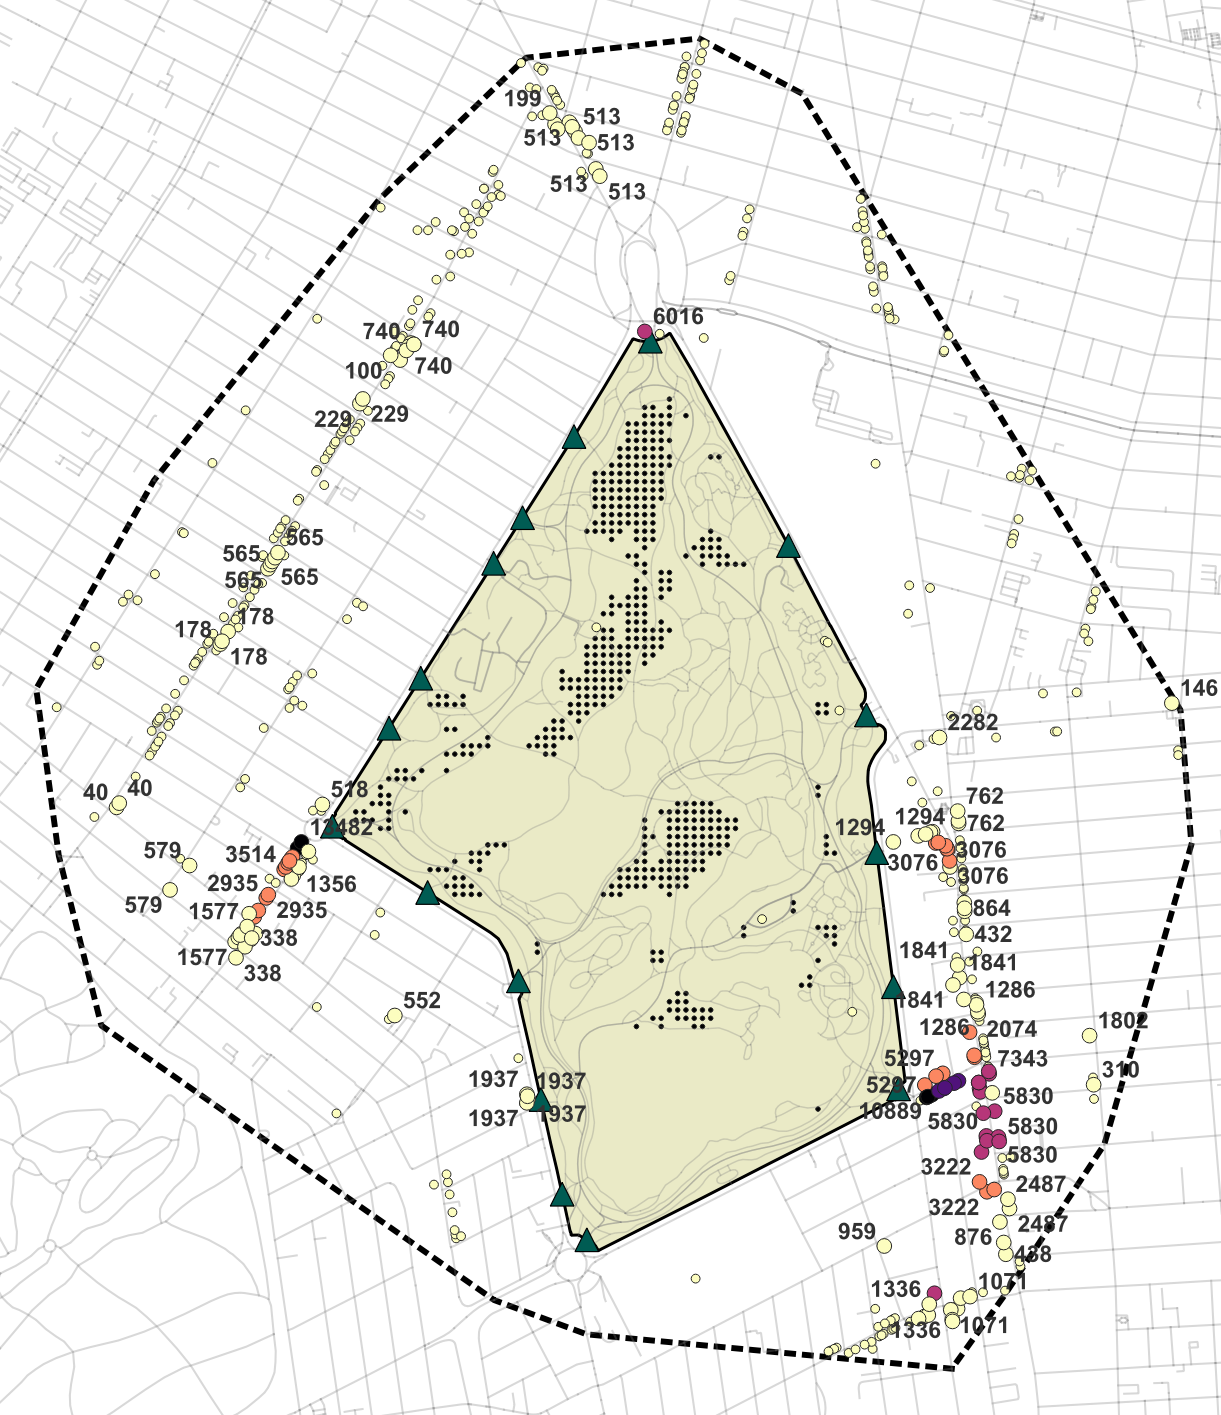
\includegraphics[width=0.8\textwidth]{images/network/prospect_betweenness_food.png} \\
  \vspace{10pt}
  \caption[Prospect Park - betweenness]{Betweenness results for food amenities surrounding Prospect Park.}
  \label{fig:prospect_betweenness_food}
\end{figure}

\begin{figure}[H]
  \centering
  \captionsetup{width=0.9\textwidth}
  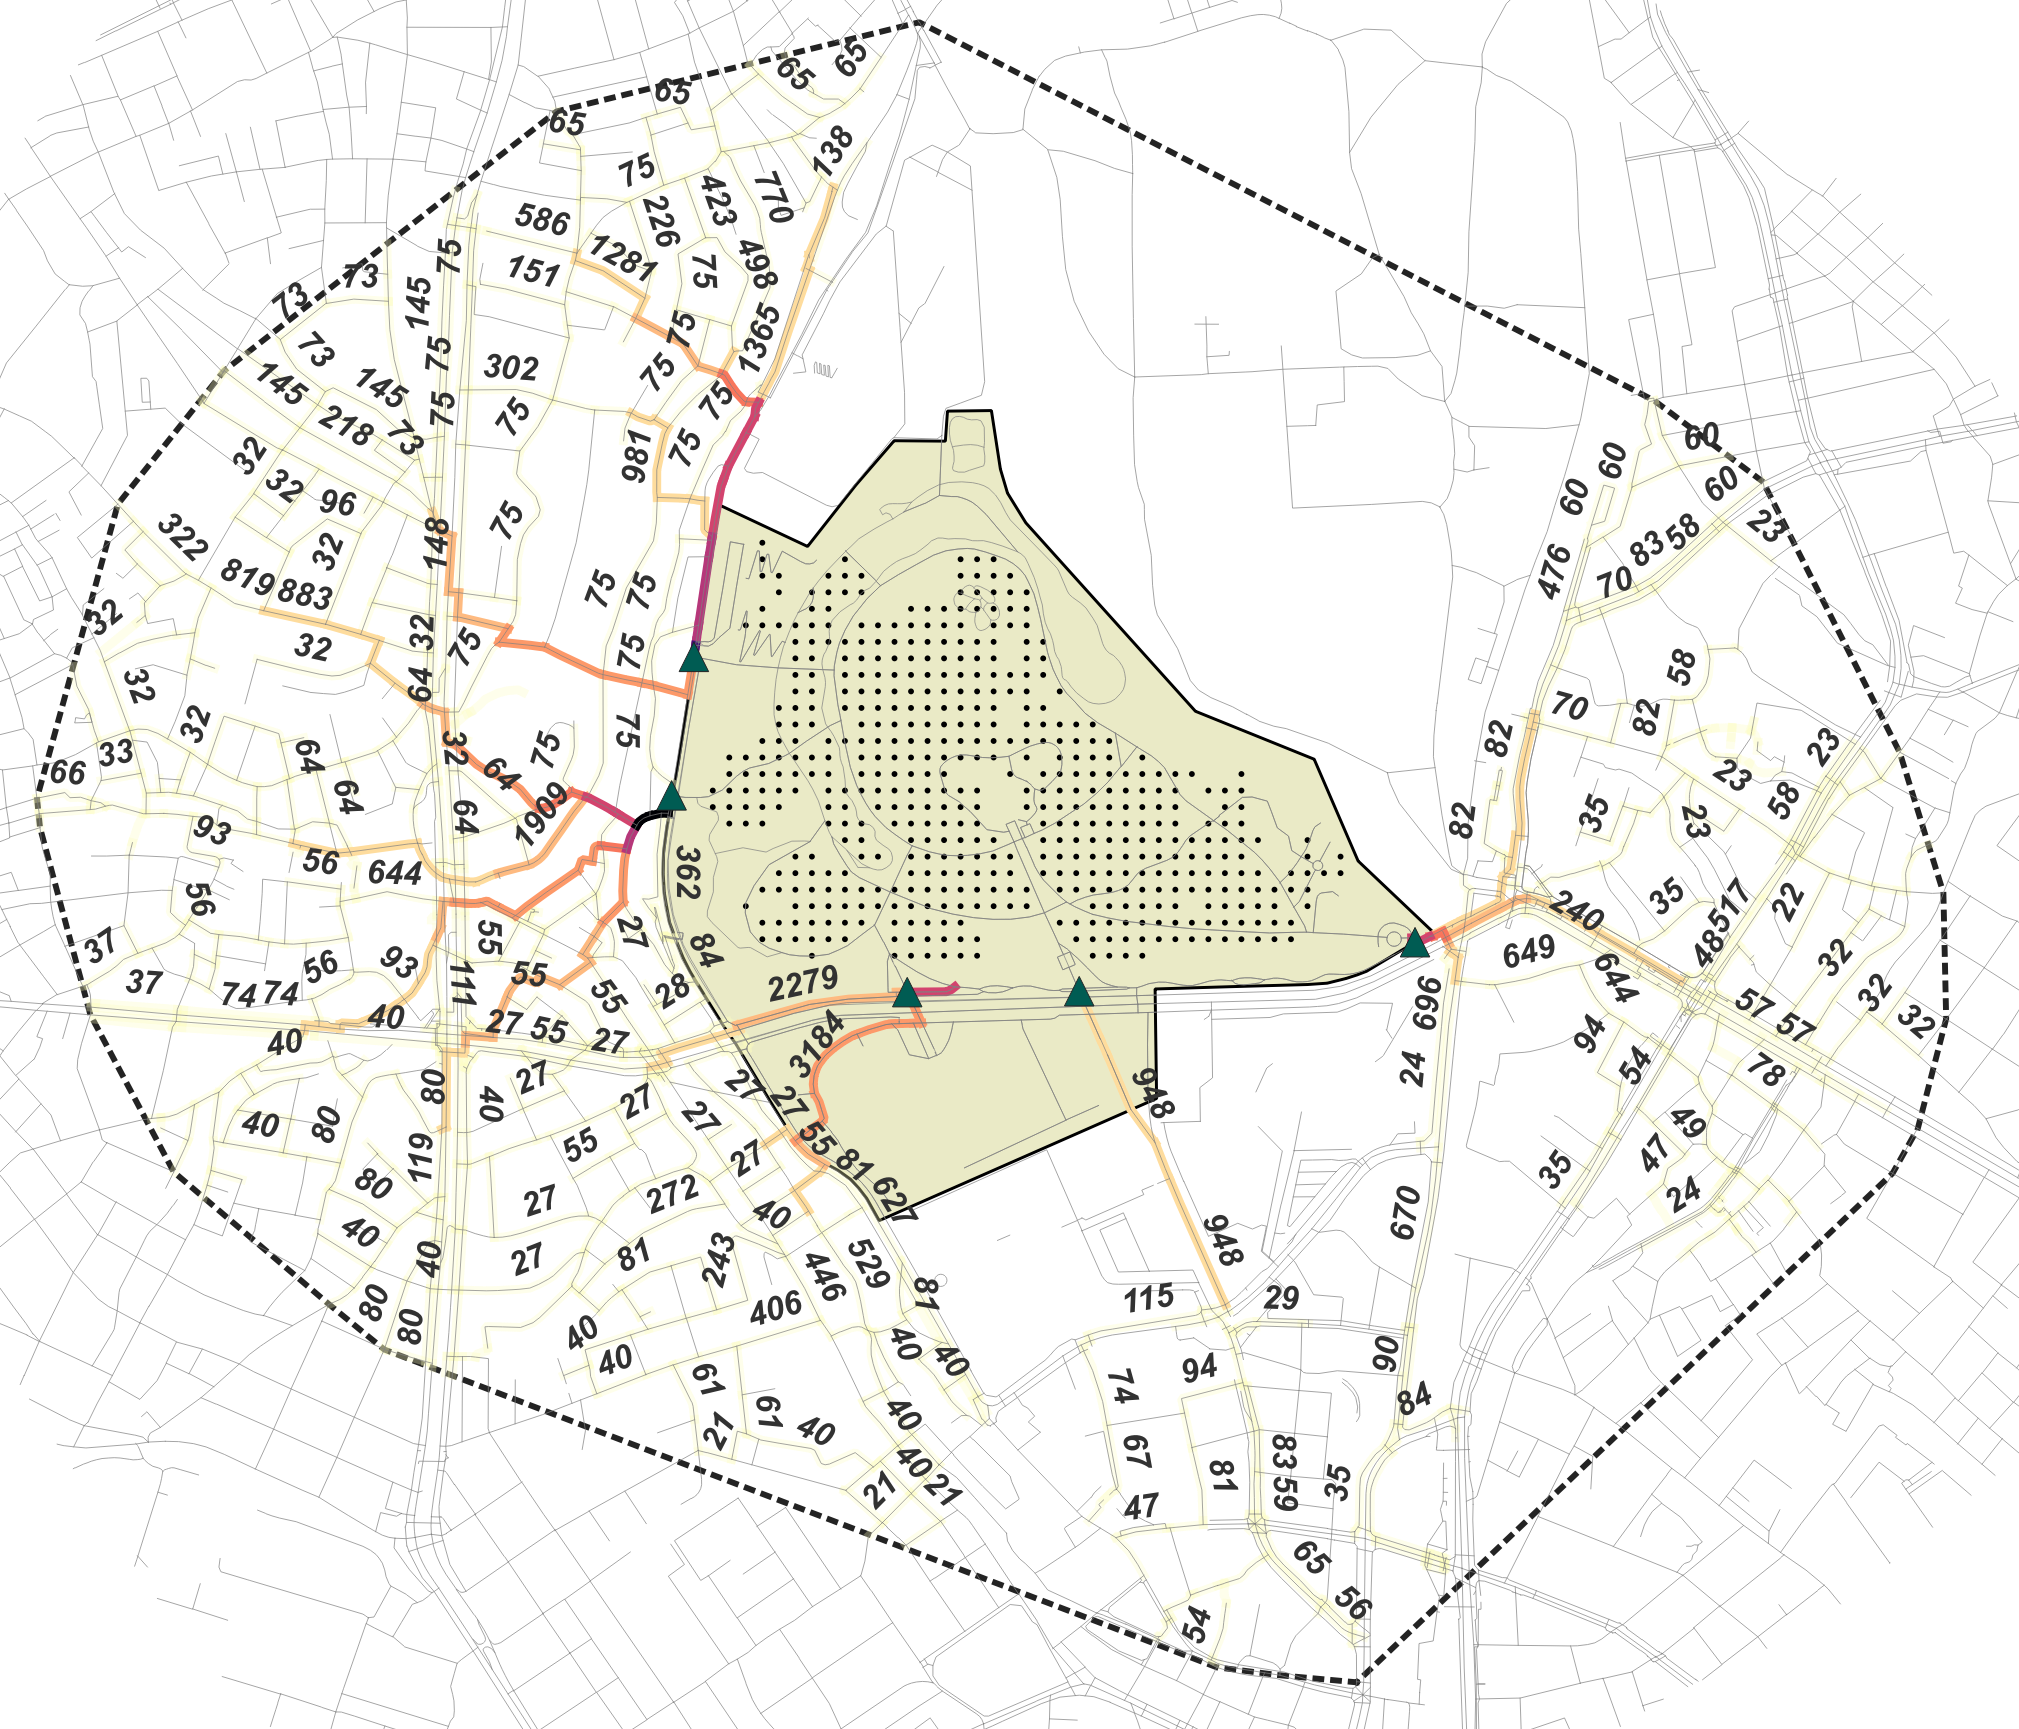
\includegraphics[width=0.9\textwidth]{images/network/yoyogi_betweenness_roads.png} \\
  \vspace{10pt} % Adjust vertical spacing between the images
  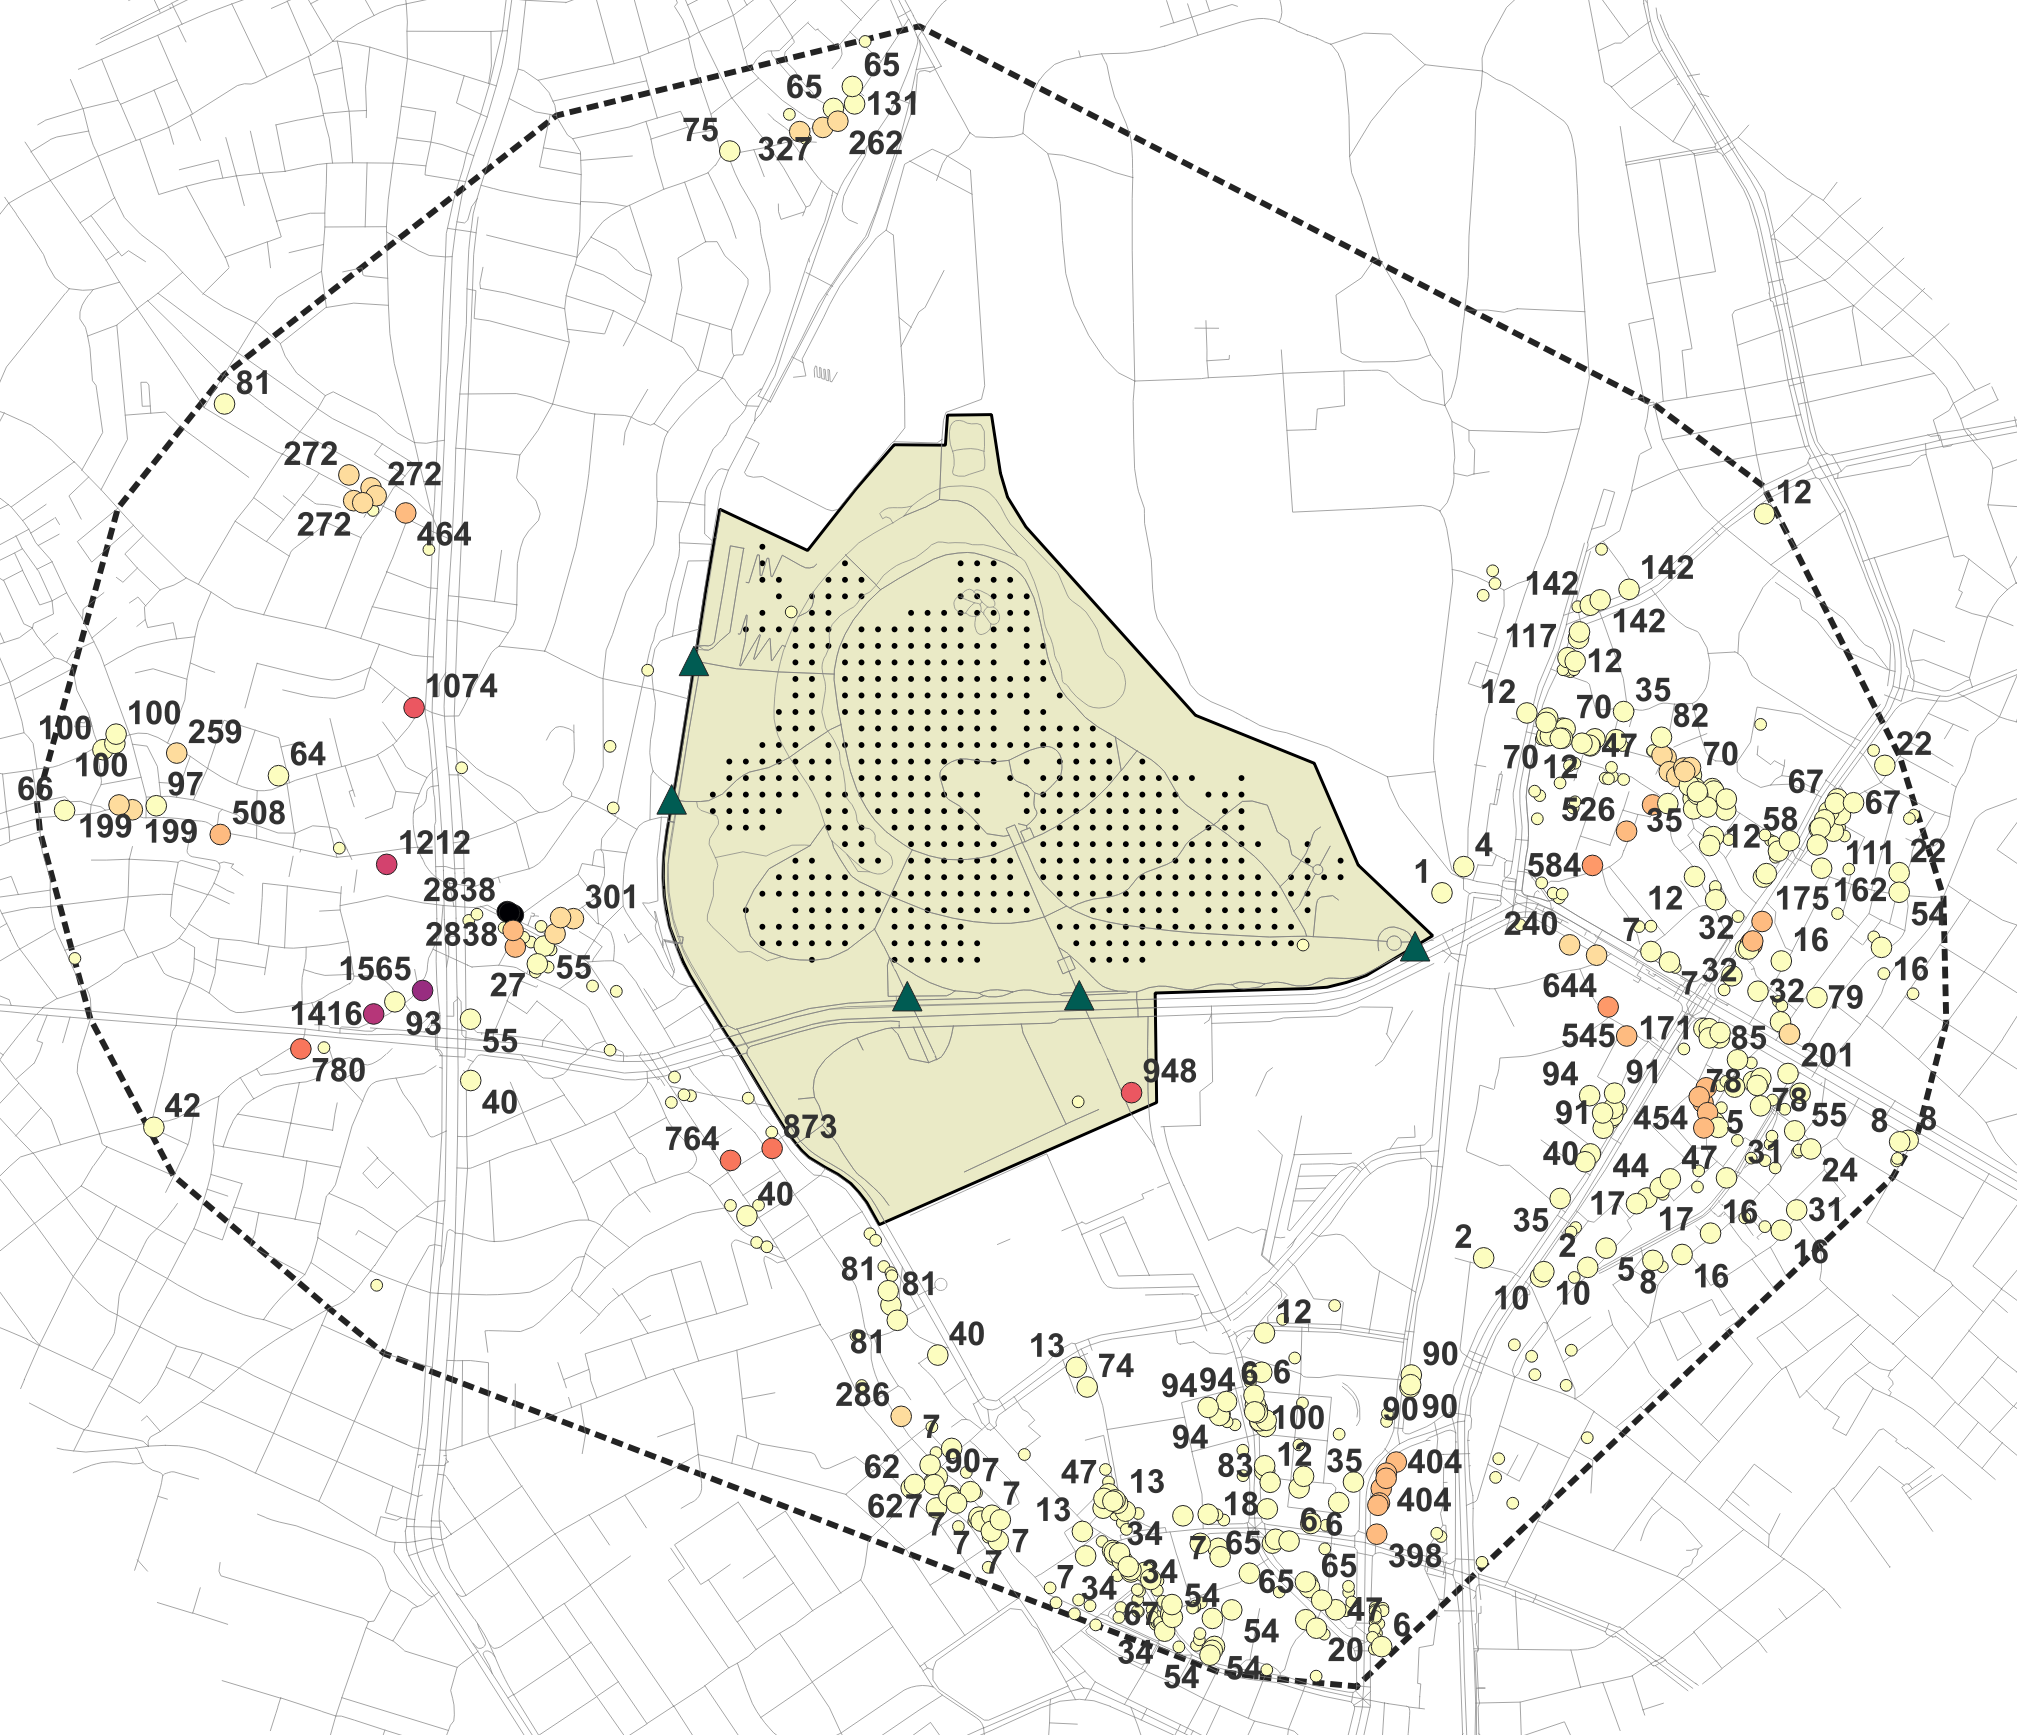
\includegraphics[width=0.9\textwidth]{images/network/yoyogi_betweenness_food.png} \\
  \vspace{10pt}
  \caption[Yoyogi Park - betweenness]{Betweenness results for network edges and food amenities surrounding Yoyogi Park.}
  \label{fig:yoyogi_betweenness}
\end{figure}

\begin{multicols}{2}

Finally, the betweenness results for Yoyogi Park in Figure \ref{fig:yoyogi_betweenness} support earlier conclusions about the high population living west of the park versus the large cluster of food amenities to the south and east. The top figure shows the network edges leading to those most populated entry points and, when compared to the bottom figure showing the food amenities, it is evident which network edges might benefit from food amenities due to the number of people utilizing those paths to arrive at Yoyogi Park. However, as it exists currently, the majority of residents traveling from home to the park and stopping for food in between will have a limited selection of food options compared to the less residential areas with the large food clusters on the opposite side of the park. 

\subsection{Cumulative distance}

The \textit{Patronage betweenness} tool in the UNA toolbox can also export tab-separated values for the cumulative length of the shortest path from each origin point to the nearest destination point. The same criteria from the betweenness results calculated above is used to calculated the the cumulative distance between the origins (intersections) and destinations (entry points) within the network boundary that accounts one-kilometer from the social gathering circles to the surrounding neighborhood. In this portion of the analysis, the cumulative length data is visualized as maps in Figure \ref{fig:network_distance} and as histograms in Figure \ref{fig:histograms} to compare the approximate population by the distance from the park entry points. 

\begin{figure}[H]
  \centering
  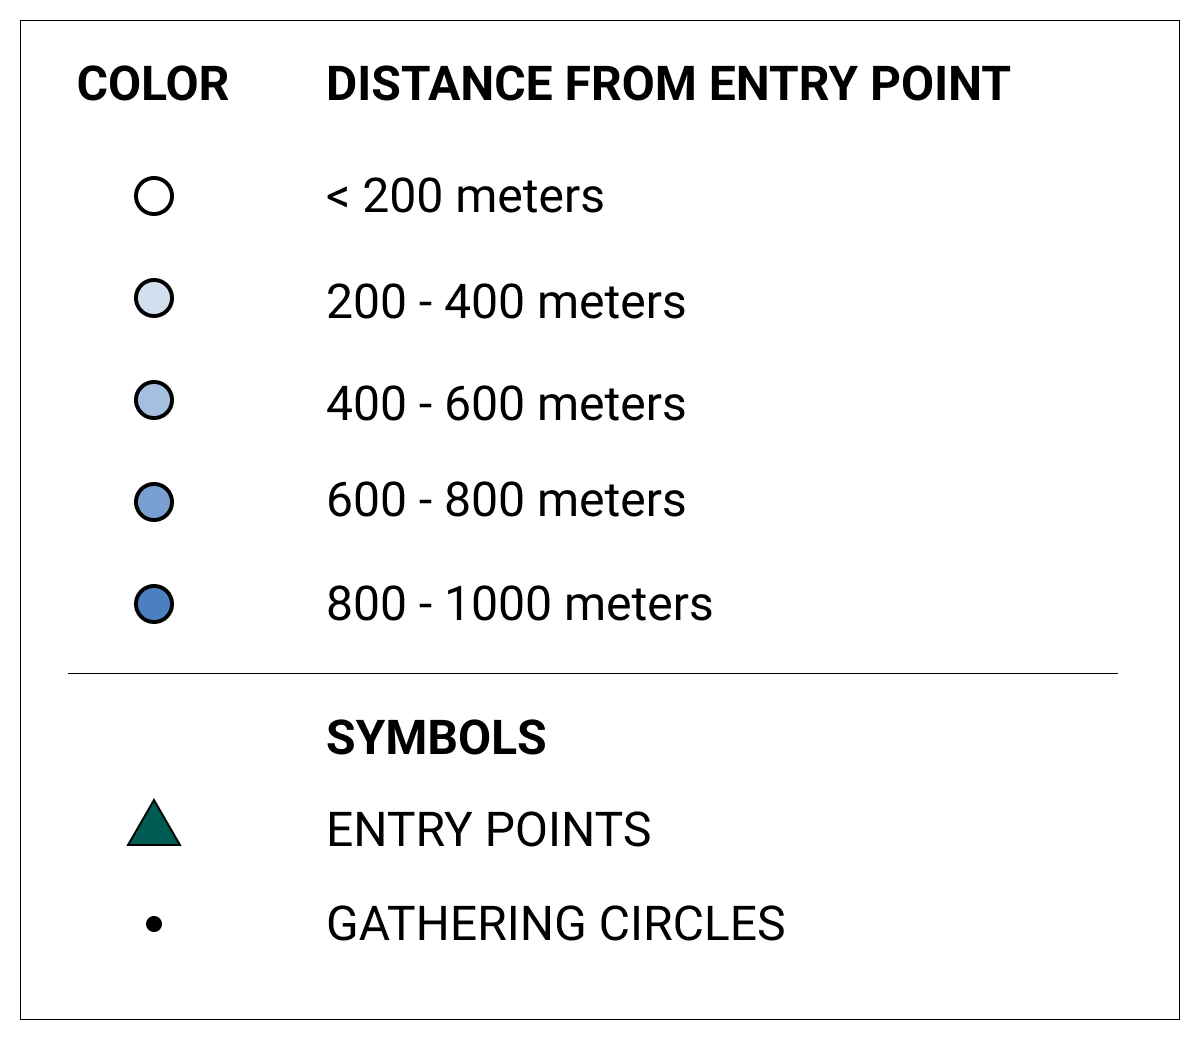
\includegraphics[width=0.45\textwidth]{images/network/distance_legend.png}\par\captionof{figure}[Distance legend]{Legend for distance analysis of population to park entry points.}
  \label{fig:distance_legend}
\end{figure} 


\begin{minipage}{0.45\textwidth}
    \centering
    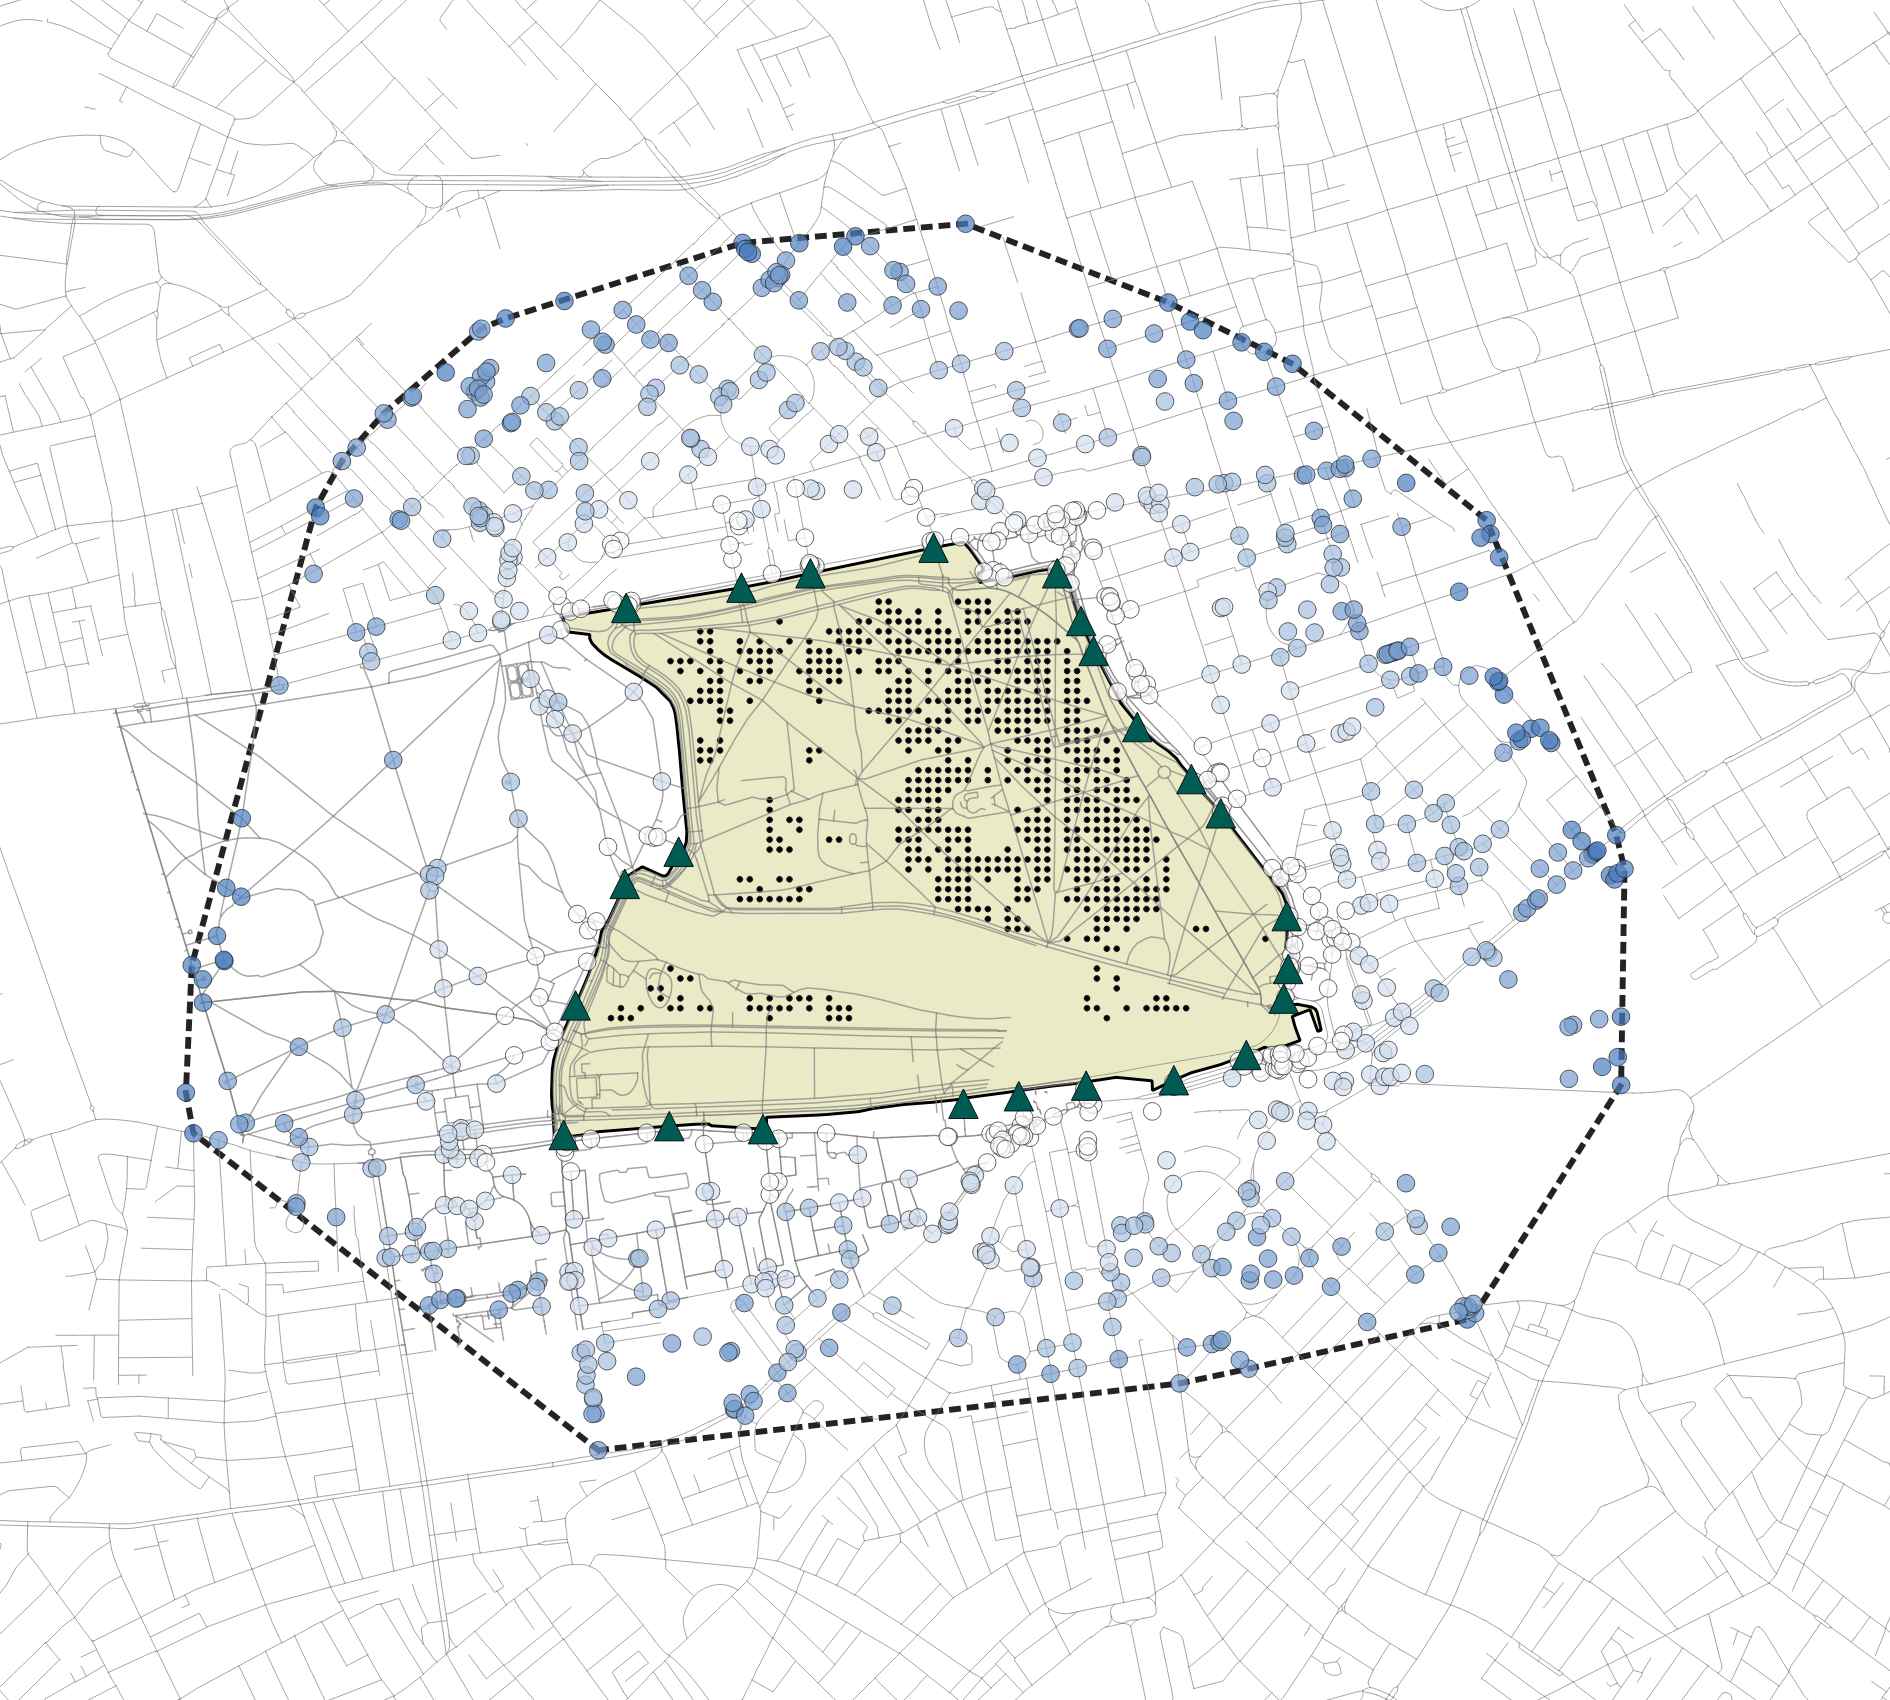
\includegraphics[width=\linewidth]{images/network/hyde_intersections_distance.png}\par\hspace{3pt}
    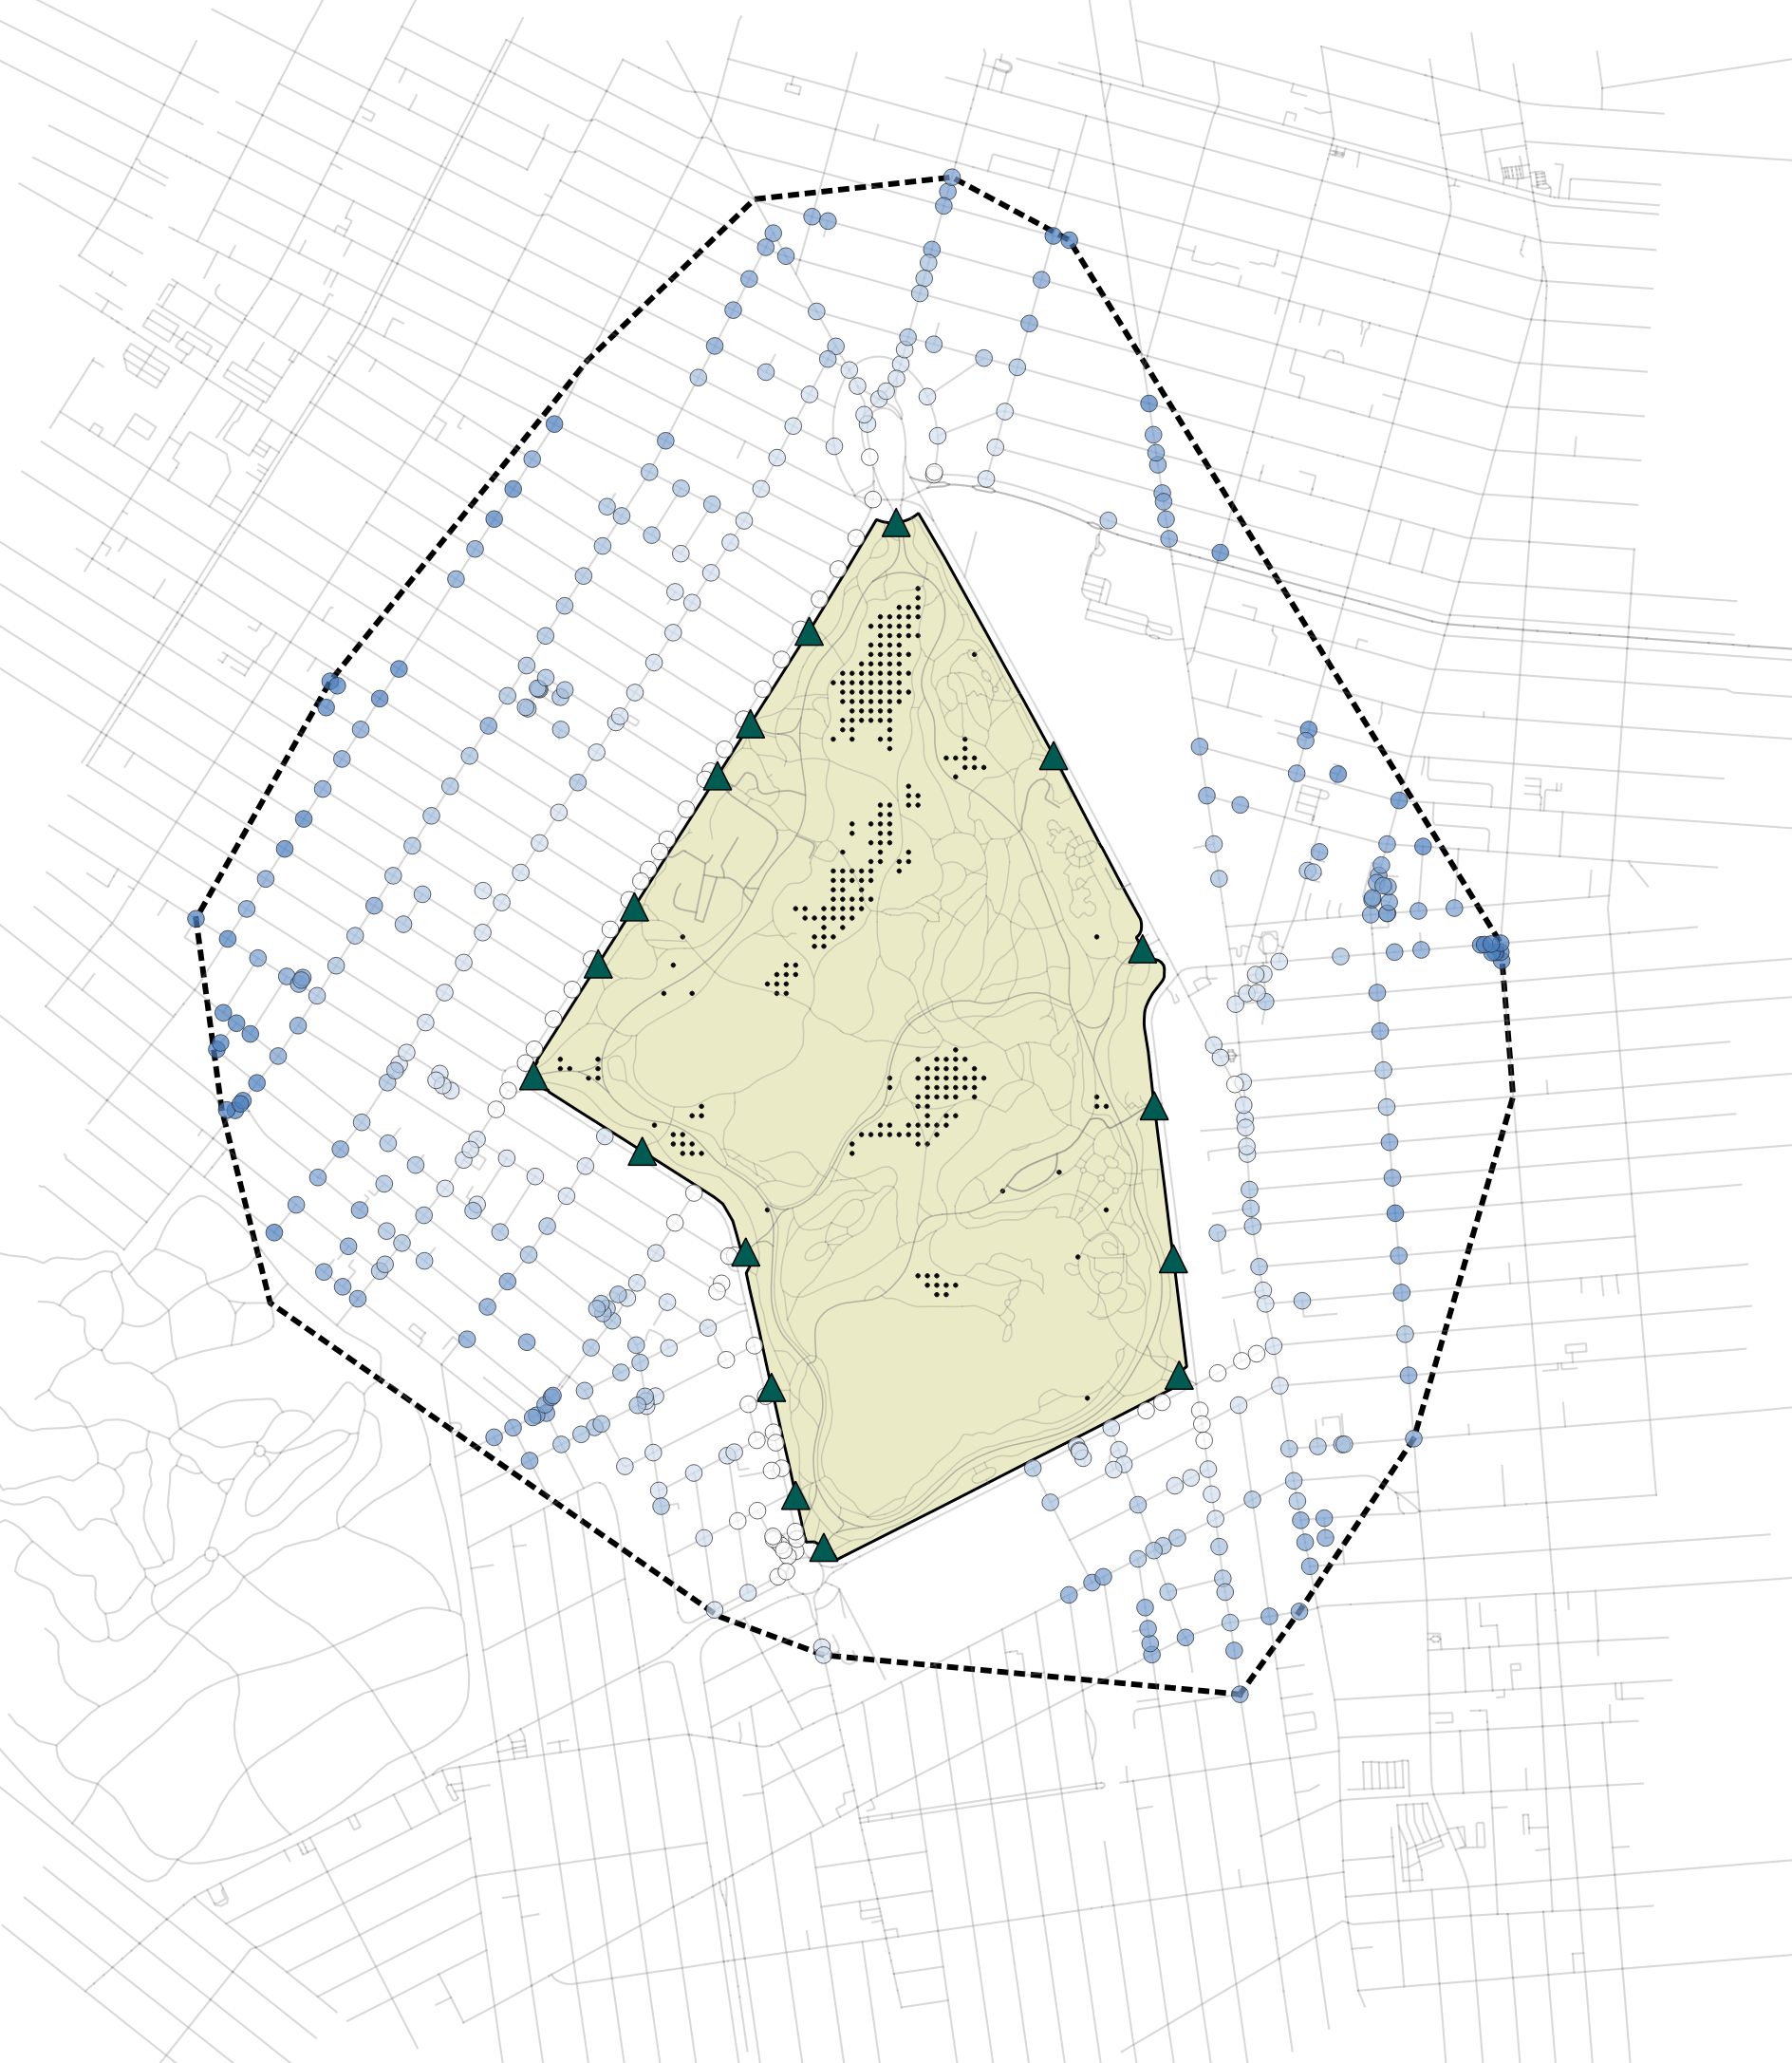
\includegraphics[width=\linewidth]{images/network/prospect_intersections_distance.png}\par\hspace{3pt}
    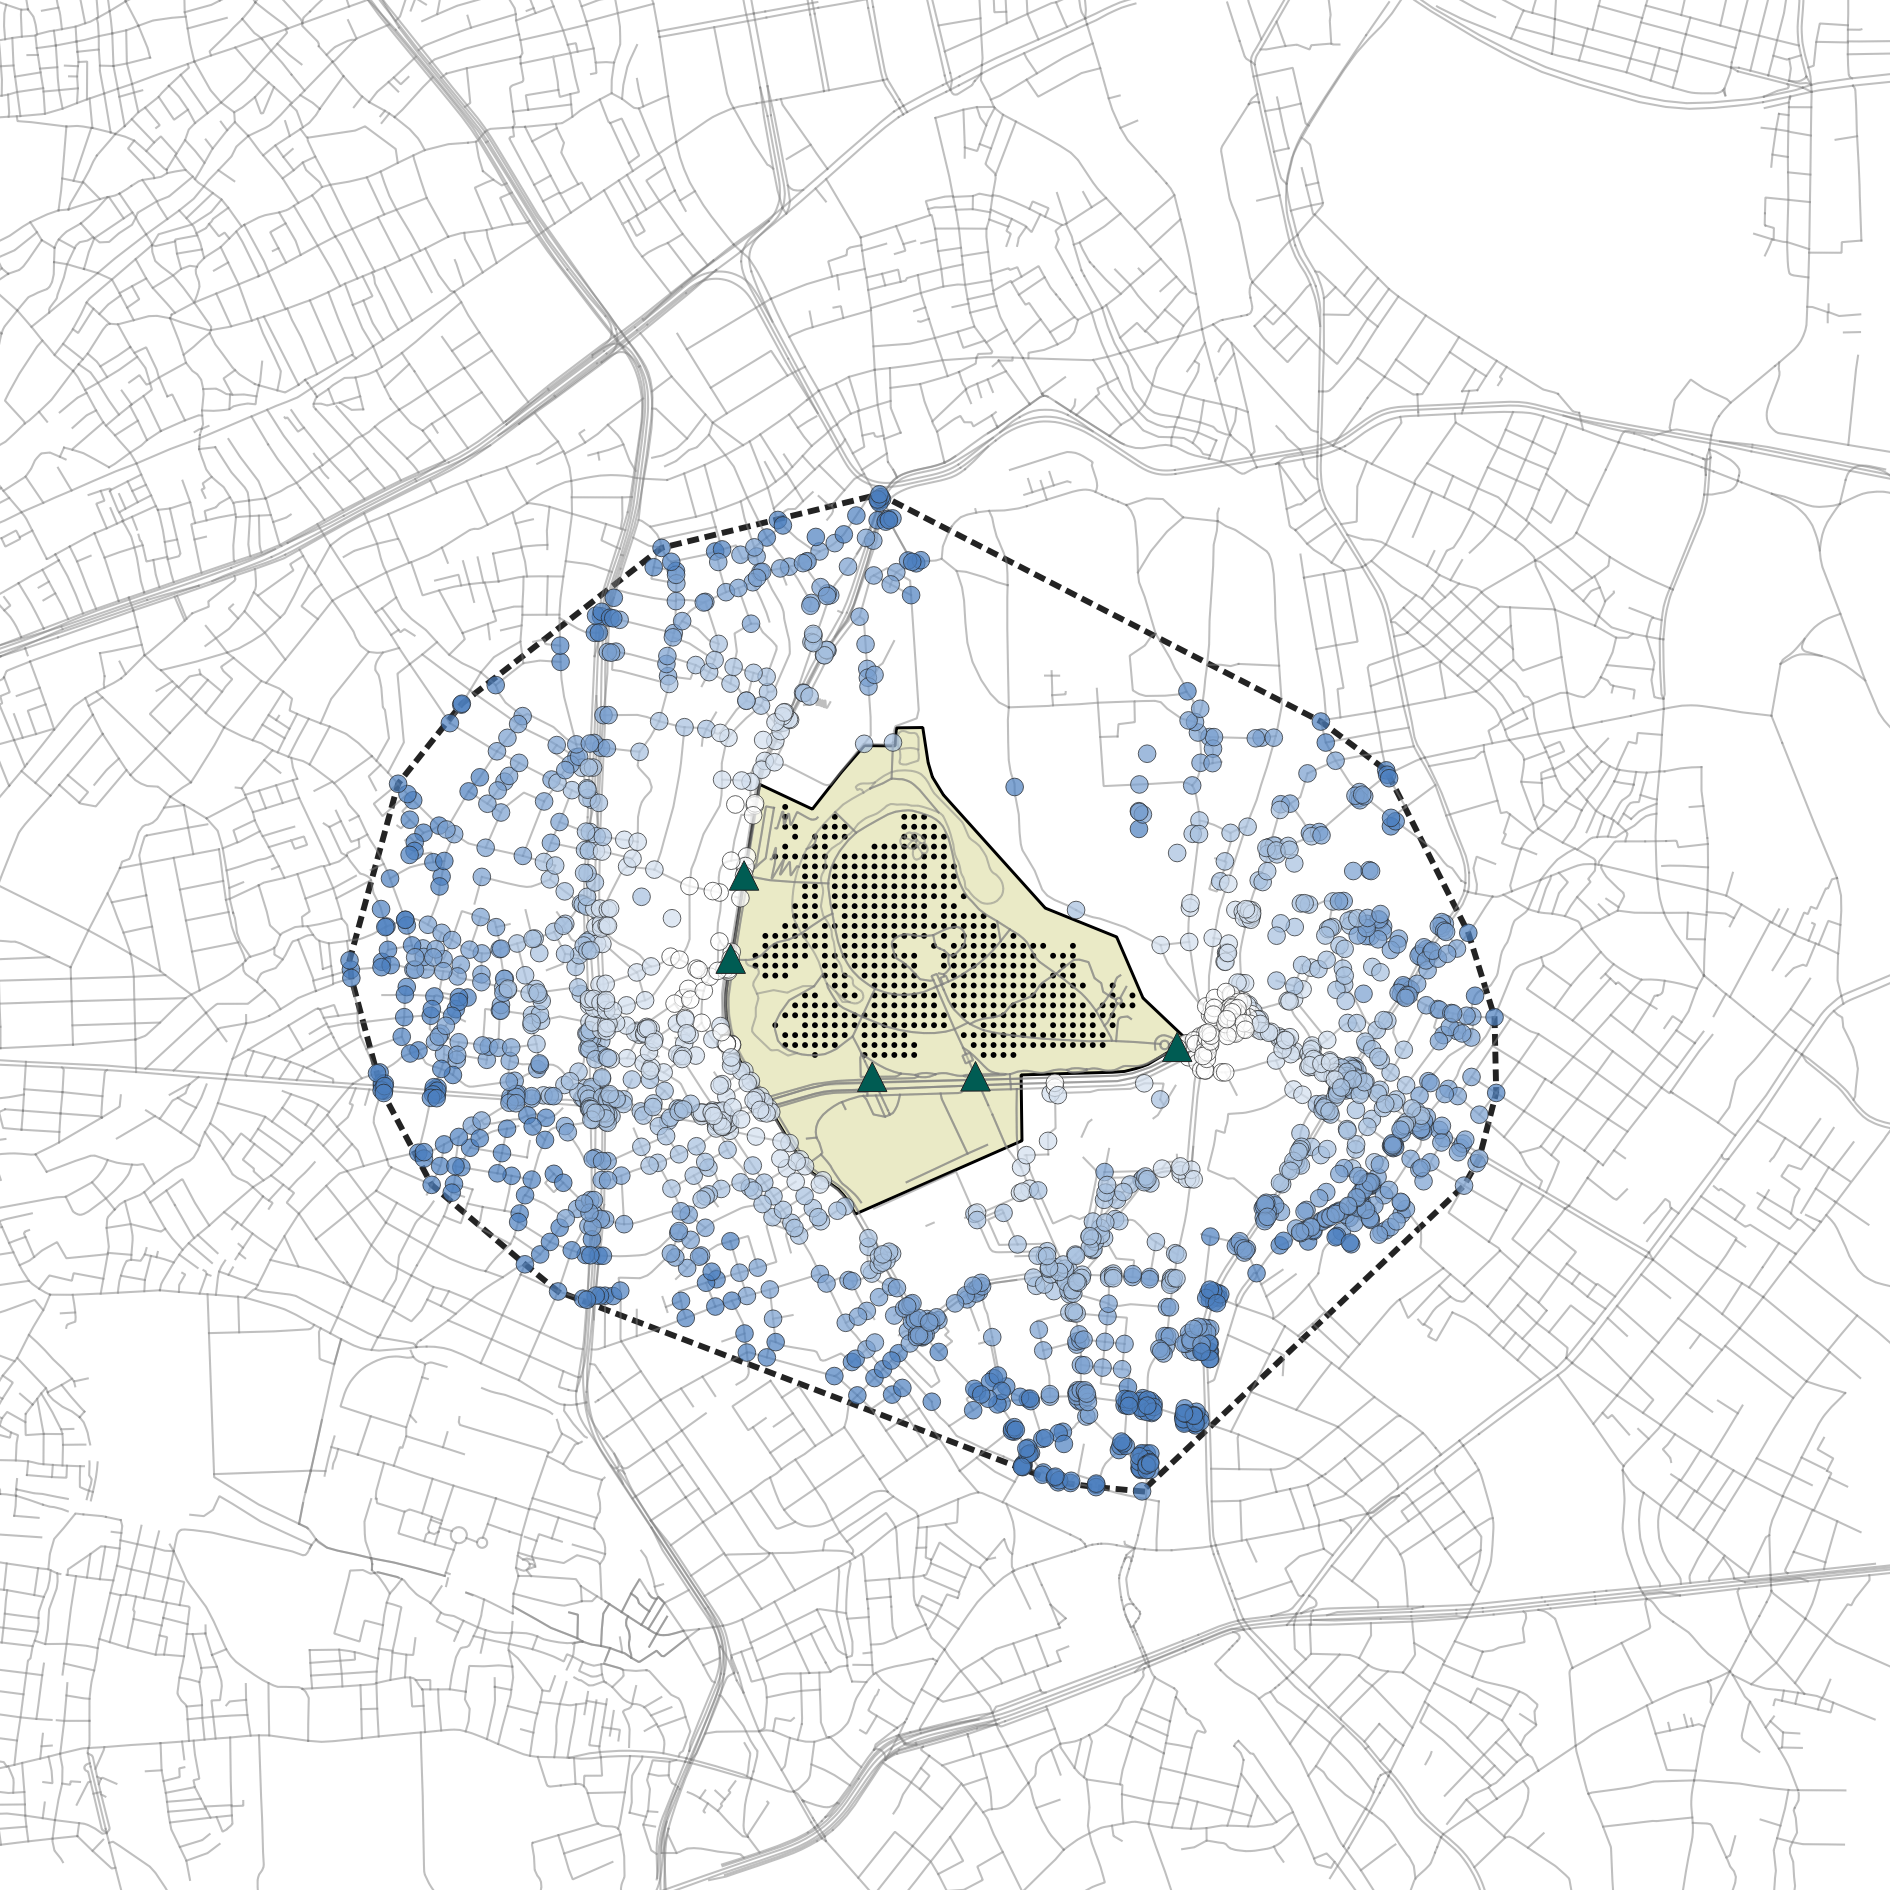
\includegraphics[width=\linewidth]{images/network/yoyogi_intersections_distance.png}\par\hspace{3pt}  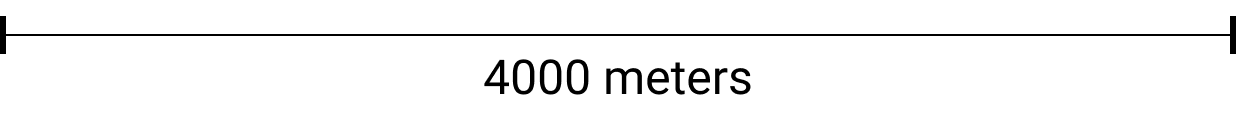
\includegraphics[width=\linewidth]
    {images/network/scale_legend_5.png}\par\captionof{figure}[Distance]{Top to bottom: Hyde Park, Prospect Park, and Yoyogi Park. Distance between intersections and park entry points, weighted by population approximations.}
    \label{fig:network_distance}
\end{minipage}

\end{multicols}

\begin{figure}[H]
  \centering
  \vspace{8pt}
  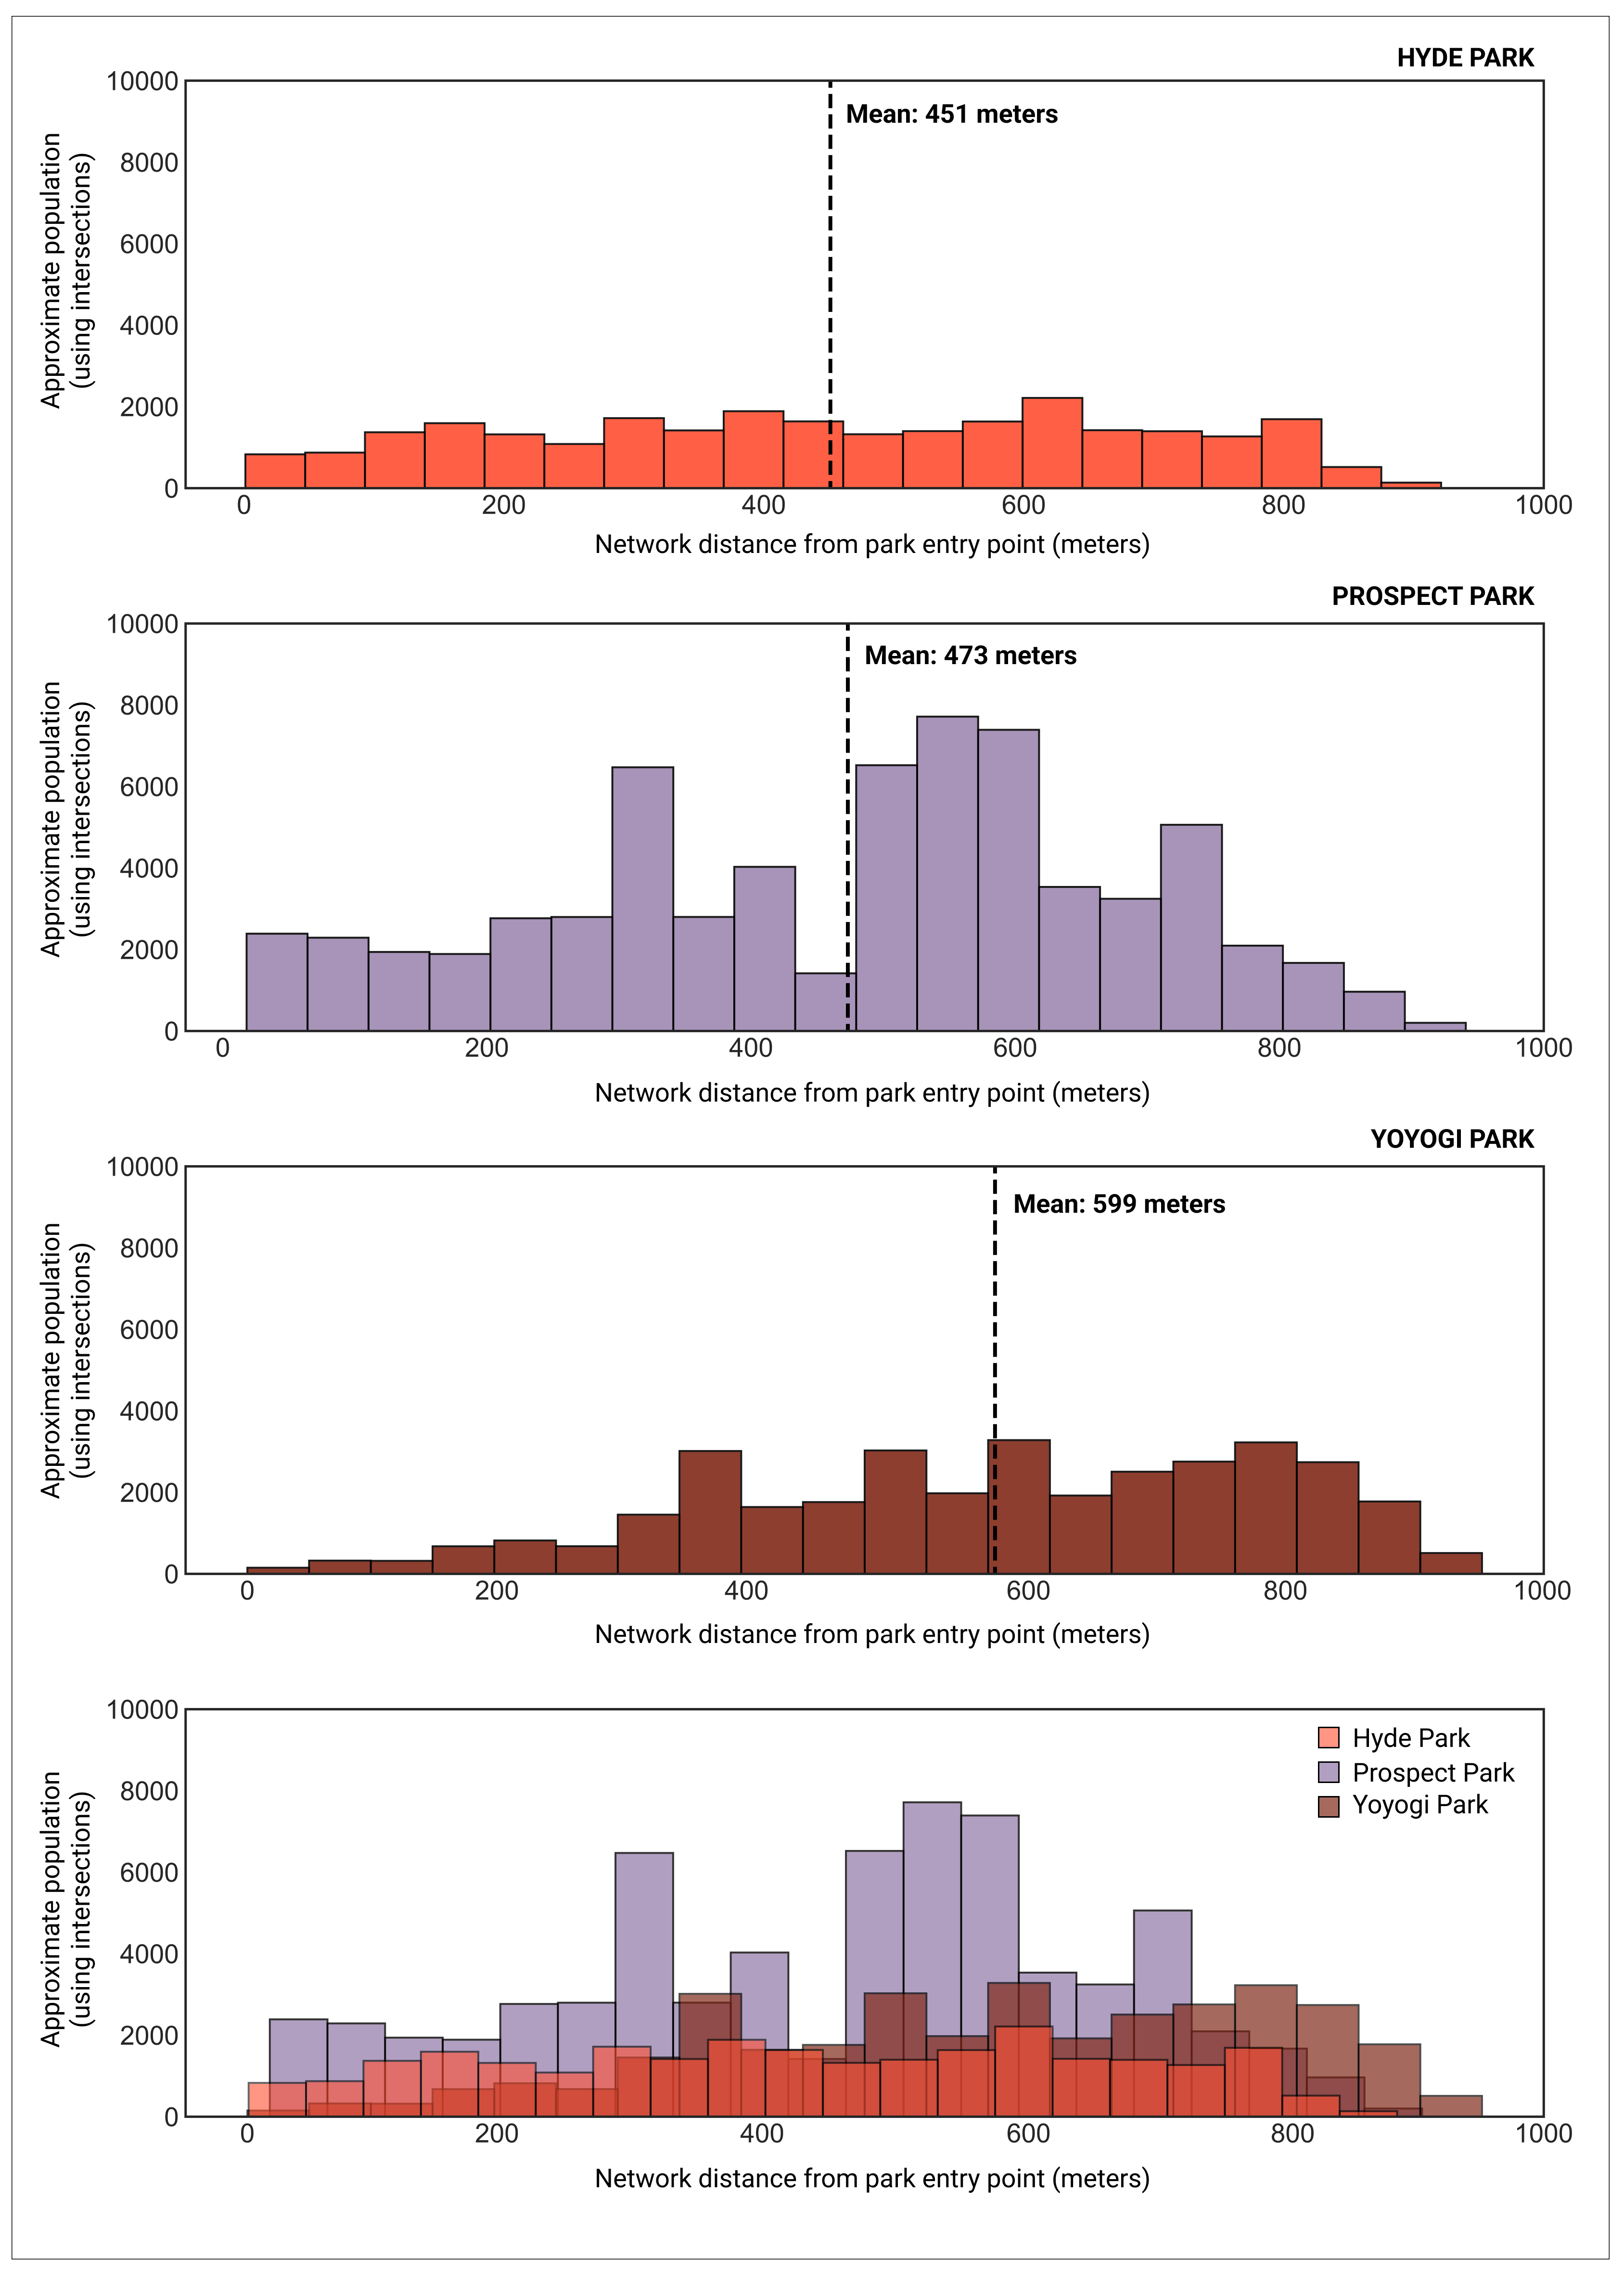
\includegraphics[width=1.0\textwidth]{images/network/histograms.png}
  \captionsetup{width=1.0\linewidth}
  \caption[Histograms of distance by population]{Approximate population by network distance from park entry points.}
  \label{fig:histograms}
\end{figure}\par
\vfill

\begin{table}[H]
\centering
\small
\begin{tabular}{llllll}
\toprule
Park name & <200m & 200-400m & 400-600m & 600-800m & 800-1000m \\
\midrule
Hyde Park     &    19.0\% &      23.0\% &      26.0\% &      26.0\% &        6.0\% \\
Prospect Park &    13.0\% &      23.0\% &      35.0\% &      24.0\% &        5.0\% \\
Yoyogi Park   &     6.0\% &      22.0\% &      32.0\% &      40.0\% &       28.0\% \\
\bottomrule
\end{tabular}
\caption[Population and entry point distances]{Percentage of the approximate population by distance from park entry point in meters.}
\label{table:distance}
\end{table}

\begin{multicols}{2}

In Figure \ref{fig:histograms}, the distributions of population for each park reinforces the findings from the population analysis, reach analysis, and betweenness analysis discussed above. Hyde Park has the most even distribution of population when looking at the distance from the entry points of the park. The weighted mean value for Hyde Park is 451 meters, which means half the population living within one-kilometer of the social gathering circles are less than a 451-meter walk to an entry point. Prospect Park has a similar weighted mean value of 473 meters, but instead of an evenly dispersed population like Hyde Park, the majority of residents (almost 60\%) around Prospect Park live between 400 and 800 meters from a park entry as seen in Table \ref{table:distance}. For Yoyogi Park, only 6\% of the population live within 200 meters of a park entry---the lowest of the three parks---and 40\% live 600-800 meters from the nearest park entry. Moreover, the weighted mean value for Yoyogi Park is 599 meters, meaning more than half of the population living within one-kilometer of a social gathering circle live more than 599 meters from a park entry point. 

Because the population analysis was studied using the social gathering circles as the starting point, all three histograms taper towards a population of zero after 900 meters. This is because the social gathering circles are located inside the park (at least 50 meters Euclidean distance from the park boundary per the conditions in Section \ref{conditions}), therefore there are no residents who live exactly one-kilometer network distance from a park entry point \textit{and} one-kilometer network distance to a social gathering circle. 

\section{Accessibility of social gatherings}
\subsection{Interpretation of the results}
In this chapter, population catchment estimation, reach analysis, and betweenness analysis are used to compare the accessibility of social gathering circles to the surrounding neighborhoods of Hyde Park, Prospect Park, and Yoyogi Park. When looking at population, social gatherings, and access to food, the results of the above analyses show Hyde Park to have the most evenly distributed entry points, population of residents, food amenities, and the most social gathering circles for the population. 

Prospect Park, as the largest park, has the highest population of residents surrounding the park but the least number of food amenities. Prospect Park also has the largest population-to-gathering-circle ratio, with one gathering circle for every nine residents. In other words, it is likely that both Prospect Park and the surrounding neighborhood are not designed in a way that maximizes the opportunity for surrounding residents to have a social gathering during a pandemic. Compared to Prospect Park, even the reduced access to food amenities on the west side of Yoyogi Park is greater than that of Prospect Park, with reach values ranging from 91-172 total food amenities within one-kilometer network distance to each entry. While Yoyogi Park has an imbalance between the geography of the surrounding residential population and the location of food amenities, the number of social gathering circles available is likely sufficient for the surrounding population during a pandemic, with one circle for every three residents. 

In the final chapter, the results from the above analysis will be discussed as well as suggestions for future research to expand the findings of this chapter. 

\end{multicols}

%why is the population distributed the way it is?